\documentclass[a5paper]{book}

\setlength\marginparwidth{30pt}

\usepackage[utf8]{inputenc}
\usepackage{t1enc}
\def\magyarOptions{defaults=hu-min}
\usepackage[magyar]{babel}
\addto\captionsmagyar{\renewcommand{\chaptername}{lecke}}

\usepackage[dvipsnames]{xcolor}
\usepackage{amsmath}
\usepackage{amsthm}
\usepackage{enumitem}
\usepackage{fancyvrb}
\usepackage[symbol]{footmisc}
\usepackage[all]{genealogytree}
\usepackage{imakeidx}
\usepackage{pdfpages}
\usepackage{storebox}
\usepackage{tcolorbox}
\usepackage{tikz}
\usetikzlibrary{trees}

% Layout for debugging
%\usepackage{showframe}

\makeindex[intoc]

% Definitions
\renewcommand{\thefootnote}{\fnsymbol{footnote}}
\renewcommand{\thempfootnote}{\fnsymbol{mpfootnote}}
\newenvironment{program}{
  \VerbatimEnvironment
  \begin{Verbatim}[frame=leftline,numbers=left,formatcom=\color{OliveGreen}]}{\end{Verbatim}
}
\newenvironment{program*}{
  \VerbatimEnvironment
  \begin{Verbatim}[frame=leftline,numbers=left,firstnumber=last,formatcom=\color{OliveGreen}]}{\end{Verbatim}
}
\newenvironment{query}{
  \VerbatimEnvironment
  \begin{Verbatim}[frame=leftline,formatcom=\color{Violet}]}{\end{Verbatim}
}
\newcommand{\pr}[1]{{\tt #1}}
\newcommand{\name}[1]{{\sc #1}}
\theoremstyle{definition}
\newtheorem{problem}{Feladat}
\newenvironment{infobox}[2]{
  \begin{tcolorbox}[center,
                    float,
                    floatplacement=ht!,
                    fonttitle=\sffamily\bfseries,
                    title={\center Kitérő: \emph{#2}},
                    width=#1\linewidth]
  }{
  \end{tcolorbox}
}

\begin{document}

\frontmatter
\pagenumbering{roman}

% Cover page

\includepdf{images/cover.pdf}

% Inside cover
\thispagestyle{empty}
\newpage

% Flyleaf
\begin{titlepage}
\thispagestyle{empty}
\centering
\vspace*{2cm}
{\large OLDD MEG PROLOGBAN!}
\end{titlepage}

% Inside cover
\thispagestyle{empty}
\newpage

% Title page
\begin{titlepage}
\centering
\vspace*{2cm}
{\Large OLDD MEG PROLOGBAN!}\\
\vspace{8cm}
{\large Salvi Péter}\\
\vspace{1em}
2022
\end{titlepage}

% Kolofon
\thispagestyle{empty}
\begin{center}
  \small
  Salvi Péter: Oldd meg Prologban!\\
  Budapest, 2022\\(\input{revision}verzió)\\
  \bigskip
  A könyv a Creative Commons \emph{Share Alike} licencnek megfelelően
  szabadon terjeszthető.
\end{center}
\vfill
\begin{center}
\begin{BVerbatim}
sárkány(N) :- sárkány(N, 'jobbra át').

sárkány(0, _) :- write('lépj egyet'), nl.
sárkány(N, X) :-
    N > 0, N1 is N - 1,
    sárkány(N1, 'jobbra át'),
    write(X), nl,
    sárkány(N1, 'balra át').

?- sárkány(14). % 16384 lépés
\end{BVerbatim}
\end{center}
\vfill
{\footnotesize Ez a könyv \LaTeX-ben készült, Computer Modern betűtípussal.\\
  A borítón egy Lindenmayer-rendszer, az ún.~\emph{sárkány görbe} látható.
}

% Ajanlas
\clearpage
\thispagestyle{empty}
\begin{center}
  \vspace*{\fill}
  {\Large\emph{Zsófinak és Julinak}}
  \vspace*{\fill}
\end{center}
\clearpage

\thispagestyle{empty}
\newpage

\addtocounter{page}{2}

\tableofcontents

\chapter{Előszó}
Ez a könyv elsősorban azoknak szól, akik még egyáltalán nem tudnak
programozni, de szeretnék megismerni a számítógépes problémamegoldás
alapjait. A ,,programozás'' ma már egy rendkívül szerteágazó
gyűjtőfogalommá vált, melynek egy-egy területe magában egy-egy szakmát
képvisel. Itt nem lesz szó webfejlesztésről, látványos játékokról vagy
neurális hálókról: kizárólag a problémamegoldásra fogunk koncentrálni,
ami viszont -- az én véleményem szerint -- a programozás
legizgalmasabb válfaja.

Ehhez a Prologot fogjuk használni. Ez az 50 éves múltra visszatekintő
programozási nyelv sokáig állt a mesterséges intelligencia kutatás
középpontjában, és bár az iparban nem hódított teret, az informatika
oktatásában továbbra is jelentős szerepe van. Ez nem véletlen: a
Prolog különösen alkalmas tanításra, ugyanis egészen minimális
ismeretekkel is már érdekes feladatok megoldását teszi lehetővé. Ezt
bizonyítják az egyes leckéket lezáró \emph{projektek} is, amelyekben
különböző, kicsit nagyobb lélegzetvételű problémákat vizsgálunk majd
meg.

\section*{Hogyan használjuk a könyvet?}
A leckékben szereplő példákat érdemes a számítógépen kipróbálni, és
kísérletezgetni velük, átírni bennük ezt--azt, és megvizsgálni, hogy mi
történik. Az efféle játék során mélyül el igazán a tudás; és ezt
segítik a feladatok is, melyeknek megoldása a könyv végén található.

Mindehhez természetesen szükség van egy Prolog fordítóra. Ezekből sok
létezik, és mindegyik meglehetősen különböző. A legtöbb azonban
kompatibilis az 1995-ös ISO szabvánnyal, és ez a könyv csak ezt
feltételezi, illetve még annyit, hogy tudja kezelni a magyar ábécé
betűit. Az ingyenesen letölthető, nyílt forráskódú rendszerek közül
ilyen az \name{SWI-Prolog}. Más implementációk, mint pl. az~\name{XSB}
vagy a \name{GNU Prolog}, jelenleg nem fogadják el az ékezetes
karaktereket, ezért ezek használata esetén a programokat ékezetek
nélkül kell begépelni.

A problémamegoldás Prologban mindig két részből áll:
\begin{enumerate}
\item Egy -- általában {\tt .pl} vagy {\tt .P} kiterjesztésű --
  fájlban megadunk egy szabályrendszert (a program
  \emph{forráskódját}). Ennek megírásához tetszőleges
  szövegszerkesztőt használhatunk.\index{forráskód}
\item Ezzel kapcsolatban a programnak felteszünk kérdéseket.
\end{enumerate}
A legtöbb Prolog rendszer indításkor mindössze egy kérdőjel kiírásával
fogad minket; ezzel jelzi, hogy várja a kérdést:
\begin{query}
?-
\end{query}  
Az első feladatunk, hogy betöltsük az általunk írt programot. Ezt
általában a \pr{consult} paranccsal tehetjük meg, például:\index{\pr{consult}}
\begin{query}
?- consult('/home/salvi/szabályok.pl').
\end{query}
\dots ahol az aposztrófok között levő {\tt /home/salvi/szabályok.pl} a
forráskód teljes elérési útja. Ne felejtsük le a parancs végéről a
pontot, majd nyomjuk meg az újsor billentyűt.

Ezután már jöhetnek a kérdések. A leckékben már csak ezek lesznek
feltüntetve, de nem szabad megfeledkezni a szabályok betöltéséről sem.
Amennyiben egy kérdésre több válasz is van, a következő választ
általában a pontosvessző ({\tt ;}) lenyomásával kaphatjuk meg, a
következő kérdés feltevéséhez pedig ilyenkor egy újsor billentyűt kell
nyomni.

Bizonyos rendszerekben mindez kényelmesebben is megtehető, így pl.~az
\name{SWI-Prolog} internetes \name{SWISH} verziójában,\footnote{\tt
https://swish.swi-prolog.org/} ahol a szabályok mindig automatikusan
újraolvasódnak.

\section*{Köszönetnyilvánítás}
Köszönettel tartozom mindenekelőtt Varga Csillának, aki lelkesen
végigcsinálta a könyvnek egy korai változatát, és kérdéseivel
rávilágított arra, hogy mit kell még pontosítanom vagy jobban
elmagyaráznom; és természetesen a feleségemnek, Iida Norikónak, akinek
a támogatása nélkül ez a könyv nem készülhetett volna el.

\begin{flushright}
  Salvi Péter\\
  Budapest, 2022.
\end{flushright}

\clearpage
\thispagestyle{empty}


\mainmatter
\pagenumbering{arabic}

% -*- fill-column: 52 -*-
% (local-set-key (kbd "C-c C-f") 'display-fill-column-indicator-mode)

\chapter{Ismerkedés}

Az első leckében egy családfa vizsgálatán keresztül
megismerkedünk a programok alkotóelemeivel és a
\emph{rekurzió}\/val.

\section{Tények}

Egy Prolog program \emph{tényekből} és
\emph{szabályokból} áll, amelyekből a számítógép
következtetéseket tud levonni. Ha megadunk egy tény-
és szabályrendszert, utána kérdéseket tehetünk fel,
amelyeket a gép legjobb tudása szerint megválaszol.

Példaként vegyük Mohamed próféta családját
(\ref{fig:csaladfa}.~ábra)!
%
\begin{figure}
  \centering
  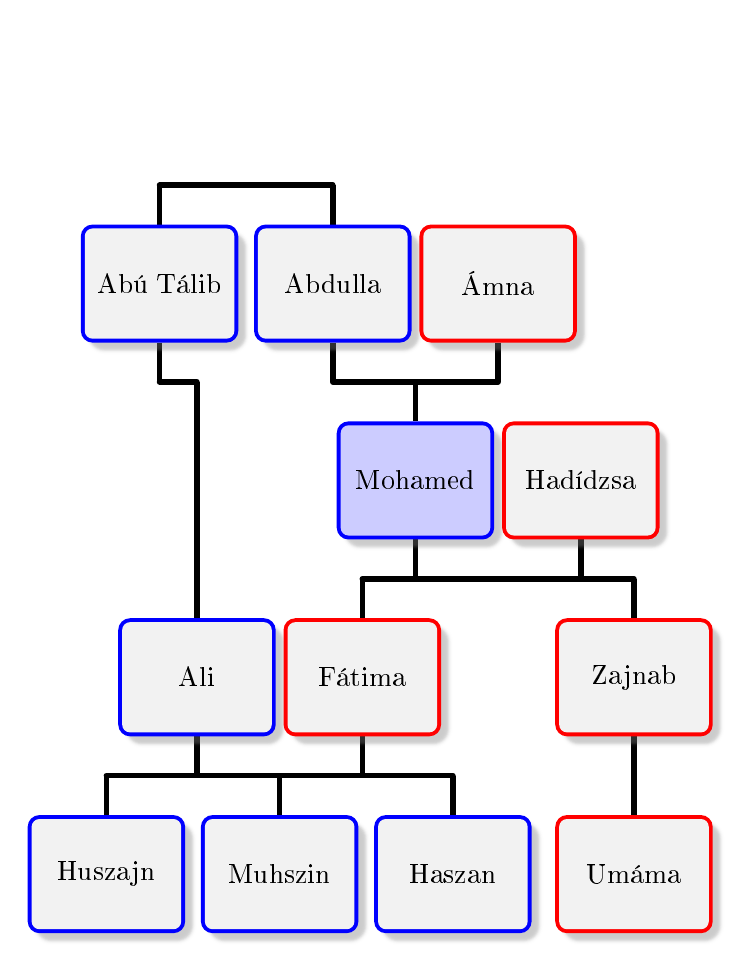
\begin{tikzpicture}
    \gtrset{edges={foreground={line width=2pt,black},no background}}
    \genealogytree[template=signpost,
                   options for node=m{box={colback=blue!20}},
                   options for family={af}{extra edges=ta{foreground={line width=2pt,black}}}]{
      child {
        g[male,phantom]{Valaki}
        c[male,id=t]{\large Abú Tálib}
        child[id=af] {
          g[male]{\large Abdulla}
          p[female]{\large Ámna}
          child {
            g[male,id=m]{\large Mohamed}
            p[female]{\large Hadídzsa}
            child {
              p[male,id=a]{\large Ali}
              g[female]{\large Fátima}
              c[male]{\large Huszajn}
              c[male]{\large Muhszin}
              c[male]{\large Haszan}
            }
            child {
              g[female]{\large Zajnab}
              c[female]{\large Umáma}
            }
          }
        }
      }
    }
  \end{tikzpicture}
  \caption{Mohamed próféta családja (részlet).}
  \label{fig:csaladfa}
\end{figure}
%
A szülő--gyerek kapcsolatokat az alábbi program
foglalja össze:

\begin{program}
szülő(abú_tálib, ali).
szülő(abdulla, mohamed).
szülő(ámna, mohamed).
szülő(mohamed, fátima).
szülő(hadídzsa, fátima).
szülő(mohamed, zajnab).
szülő(hadídzsa, zajnab).
szülő(ali, huszajn).
szülő(fátima, huszajn).
szülő(ali, muhszin).
szülő(fátima, muhszin).
szülő(ali, haszan).
szülő(fátima, haszan).
szülő(zajnab, umáma).
\end{program}

Ebben a programban minden sor egy \emph{tény}. Egy
tény dolgok (itt emberek) közti kapcsolatot ír le. A
formája a következő: a kapcsolat nevével kezdődik
(most ez a \pr{szülő}), utána zárójelek között
vesszővel elválasztva felsoroljuk a kapcsolatban
levő dolgokat, és a végén egy ponttal (\pr{.})
zárjuk.\index{tény}

Talán furcsa lehet, hogy minden kisbetűvel van --
majd később lesz szó arról, hogy mik az elnevezés
pontos szabályai, egyelőre azt jegyezzük meg, hogy
minden \emph{konkrét} dolog kisbetűvel írandó, és
nem lehet benne szóköz.

\begin{infobox}{.75}{Mohamed családfája}
A programban a családfának csak egy nagyon kis
szeletét használtuk, és még ezen a részen belül
sem tartalmaz minden kapcsolatot, mert pl.~Ali
Fátima halála után feleségül vette Umámát is.

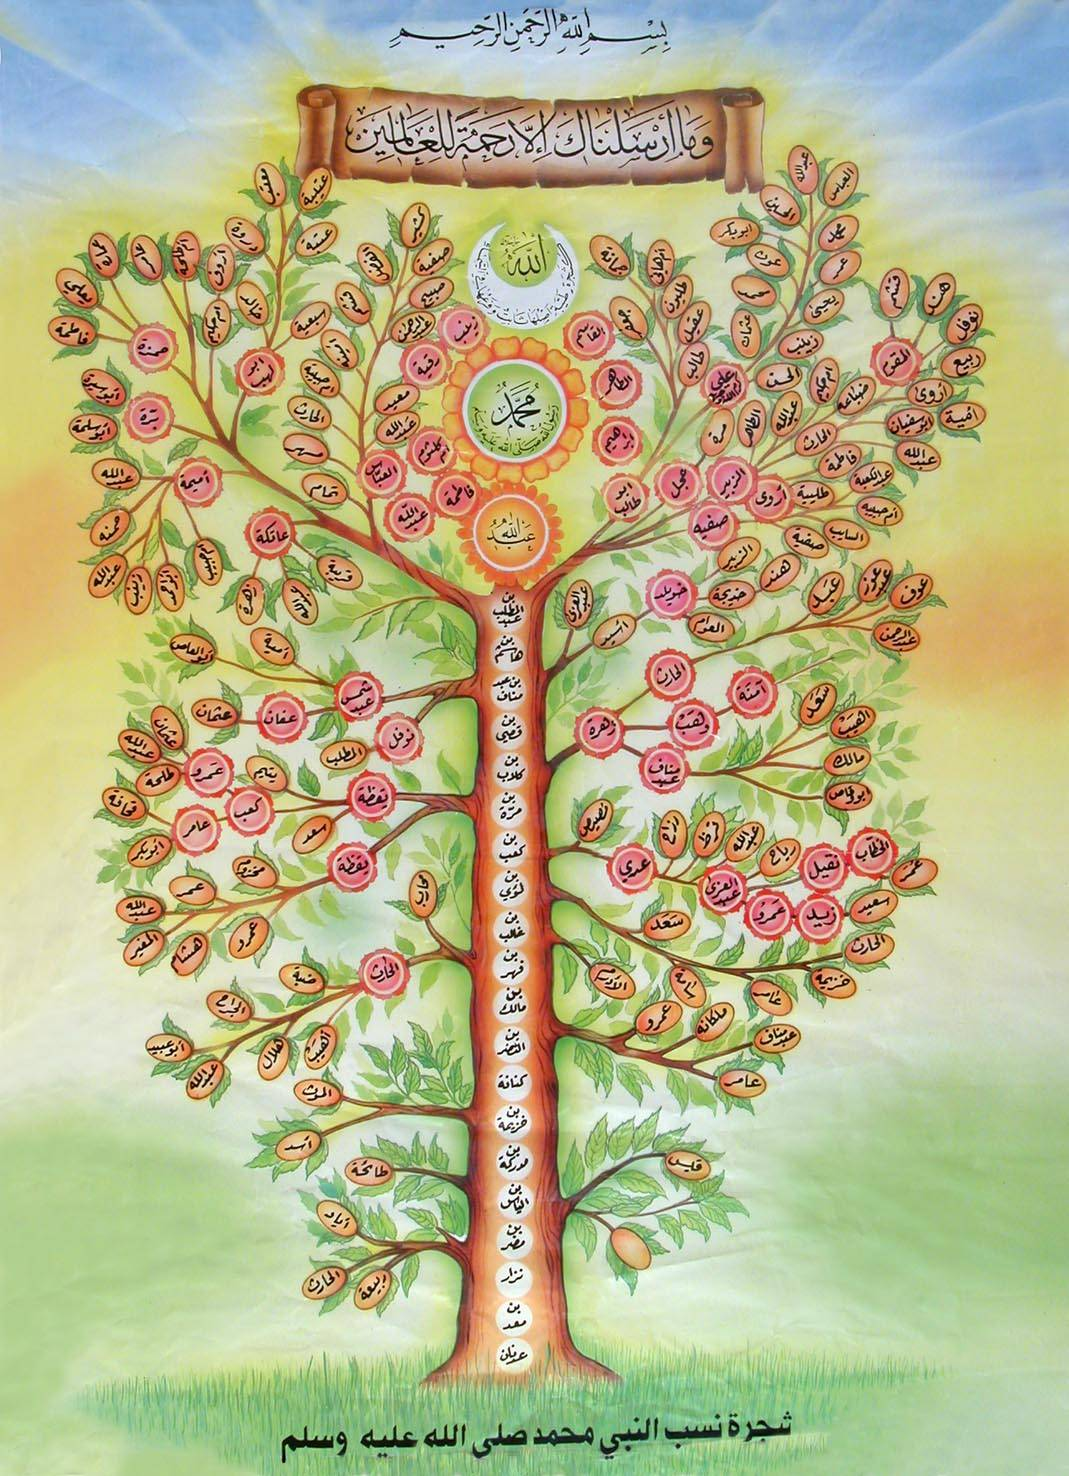
\includegraphics[width=\textwidth]{images/prophet-family.jpg}
\end{infobox}

\subsection*{Egyszerű kérdések}

Már egy ilyen egyszerű program esetén is lehet
értelmes kérdéseket feltenni. Például
megkérdezhetjük, hogy
\begin{query}
?- szülő(mohamed, fátima).
\end{query}
\dots amire a rendszer a \pr{true} (igaz) vagy
\pr{yes} (igen) üzenettel
válaszol;\index{\pr{true}}\index{\pr{yes}} vagy hogy
\begin{query}
?- szülő(ali, zajnab).
\end{query}
\dots amire a \pr{false} (hamis) vagy \pr{no} (nem)
eredményt adja.\index{\pr{false}}\index{\pr{no}} (A
továbbiakban ez a könyv a \pr{true} és \pr{false}
válaszokat fogja használni.)

Egy kicsit érdekesebb a következő kérdés:
\begin{query}
?- szülő(mohamed, Kicsoda).
\end{query}
Erre azt a feleletet kapjuk, hogy \pr{Kicsoda =
  fátima}. Ha további válaszokat kérünk, akkor még
azt is kiírja alá, hogy \pr{Kicsoda = zajnab}.

Mi történt itt? Azáltal, hogy a második helyre egy
nagybetűs szót (\pr{Kicsoda}) írtunk, azt mondtuk,
hogy ez egy határozatlan, ismeretlen érték, egy
\emph{változó}.\index{változó} A kérdést tehát
magyarul úgy lehetne megfogalmazni: ,,Mohamed kinek
a szülője?''

Erre megkeresi az első választ, amit talál
(\pr{fátima}), és ha továbbit kérünk tőle, akkor
megtalálja \pr{zajnab}ot is, és látja, hogy nincs
több, és így leáll.

Ha kisbetűvel írtuk volna:
\begin{query}
?- szülő(mohamed, kicsoda).
\end{query}
\dots akkor a \pr{false} eredményt kaptuk volna,
hiszen \pr{kicsoda} itt egy konkrét dolgot jelöl, a
kérdés tehát azt jelenti: ,,Igaz-e, hogy Mohamed
szülője Kicsodának?''

A kérdés a másik irányban is feltehető:
\begin{query}
?- szülő(Ki, ali).
\end{query}
\dots tehát ,,Ki Ali szülője?'', amire a \pr{Ki =
  abú\_tálib} feleletet kapjuk.

Még tovább is mehetünk, és rákérdezhetünk az összes
szülő-gyerek kapcsolatra:
\begin{query}
?- szülő(Ki, Kinek).
\end{query}
\dots azaz ,,Ki kinek a szülője?''. Az első válasz
az lesz, hogy
\begin{query}
Ki = abú_tálib,
Kinek = ali
\end{query}
További válaszok kérésével sorban megkapjuk az
adatbázisunk minden egyes elemét.

\subsection*{Összetett kérdések}

Tegyük fel, hogy arra vagyunk kíváncsiak, hogy kik
Mohamed unokái. Hogyan tudjuk ezt megkérdezni? Az
unoka definíció szerint a gyerek gyereke, tehát
tudjuk, hogy van valaki, aki szülője az unokának, és
akinek a szülője Mohamed. A logikai \emph{és}\/sel
összekötött, együtt teljesítendő feltételeket
vesszővel választjuk el:
\begin{query}
?- szülő(mohamed, Valaki), szülő(Valaki, Unoka).
\end{query}
Négy megoldást is kapunk:
\begin{query}
Unoka = huszajn,
Valaki = fátima
Unoka = muhszin,
Valaki = fátima
Unoka = haszan,
Valaki = fátima
Unoka = umáma,
Valaki = zajnab
\end{query}
(Ezek páronként értendők, tehát Fátimától van
Huszajn, Muhszin és Haszan, és Zajnabtól Umáma.)

Ez azért működik, mert egy változónak minden
előfordulása azonos értéket kell, hogy kapjon.
A kérdés két tagjának sorrendje felcserélhető, tehát
ugyanezt az eredményt adja ez is:
\begin{query}
?- szülő(Valaki, Unoka), szülő(mohamed, Valaki).
\end{query}
(Majd látni fogjuk viszont, hogy a számításigényük
nem azonos, érdemesebb az erősebb megszorítással
kezdeni.)

Hasonlóan rákérdezhetünk, hogy kik Huszajn
nagyszülei:
\begin{query}
?- szülő(Valaki, huszajn), szülő(Nagyszülő, Valaki).
\end{query}
\dots amire megkapjuk Abú Tálibot, Mohamedet és
Hadídzsát.

Ha arra vagyunk kíváncsiak, hogy Haszan testvére-e
Huszajnnak, így fogalmazhatjuk meg:
\begin{query}
?- szülő(Valaki, haszan), szülő(Valaki, huszajn).
\end{query}
Azt kapjuk, hogy \pr{Valaki = ali}, tehát a válasz
igen. Ha \pr{huszajn} helyett \pr{abdullá}t írunk,
akkor \pr{false} választ kapunk.

\begin{problem}
Válaszold meg az alábbi kérdéseket!
\begin{enumerate}
\item \pr{?- szülő(huszajn, X).}
\item \pr{?- szülő(X, huszajn).}
\item \pr{?- szülő(ámna, X), szülő(X, fátima).}
\item \pr{?- szülő(ámna, X), szülő(X, Y), szülő(Y, haszan).}
\end{enumerate}
\end{problem}
\begin{problem}
Fogalmazd meg Prologban!
\begin{enumerate}
\item Ki Ali szülője?
\item Umámának van gyereke?
\item Ki Zajnab nagyszülője?
\end{enumerate}
\end{problem}
\begin{problem}
Készítsd el a saját családfádat (nagyszülőkig
és unokatestvérekig)!
\end{problem}

\section{Szabályok}

Eddig csak tényekkel foglalkoztunk, de valójában a
Prolog programok nagy része \emph{szabályokból}
áll. Először is egészítsük ki a programunkat a
szereplőink nemével!\index{szabály}

\begin{program}
férfi(abú_tálib).
férfi(abdulla).
férfi(mohamed).
férfi(ali).
férfi(huszajn).
férfi(muhszin).
férfi(haszan).

nő(ámna).
nő(hadídzsa).
nő(fátima).
nő(zajnab).
nő(umáma).
\end{program}

Ha most a \pr{szülő} mellett szeretnénk \pr{anya} és
\pr{apa} kapcsolatokat is létrehozni, ezt
megtehetjük egyenként:
\begin{program}
anya(ámna, mohamed).
anya(hadídzsa, fátima).
...
apa(abú_tálib, ali).
apa(abdulla, mohamed).
...
\end{program}
Ez azonban elég sok munka, és érezzük, hogy
felesleges, hiszen kikövetkeztethető.  Szabályok
segítségével ezt sokkal egyszerűbben megoldhatjuk:
\begin{program}
anya(X, Y) :- szülő(X, Y), nő(X).
apa(X, Y) :- szülő(X, Y), férfi(X).
\end{program}
A \pr{:-} jelet itt úgy olvashatjuk ki, hogy
,,akkor, ha'', tehát ,,X anyja Y-nak akkor, ha X
szülője Y-nak és X nő''. A baloldalon levő részt a
szabály \emph{fej}\/ének, a jobboldalát a szabály
\emph{törzs}\/ének nevezzük.\index{fej}\index{törzs}

Mi történik, amikor feltesszük az alábbi kérdést?
\begin{query}
?- anya(ámna, mohamed).
\end{query}
A rendszer megtalálja az \pr{anya} szabályt, és
\emph{egyesíti} az \pr{X}-et \pr{ámná}\-val, az
\pr{Y}-t pedig \pr{mohamed}del.\index{egyesítés} (Az
egyesítésről még később szó lesz, itt egyszerűen
helyettesítést jelent.) Ezután megnézi, hogy a
szabály jobboldalán levő feltétel teljesül-e; ez
most a
\begin{query}
szülő(ámna, mohamed), nő(ámna).
\end{query}
\dots és ezek a tények szerepelnek a programban,
tehát \pr{true} válasszal tér vissza.

Definiáljuk a ,,nagyszülő'' kapcsolatot!
\begin{program}
nagyszülő(X, Z) :- szülő(X, Y), szülő(Y, Z).
\end{program}
Ez pontosan követi azt, ahogy megkerestük valakinek
a nagyszülőjét.

\subsection*{Problémás esetek}

Hogyan tudnánk megadni a ,,fivér'' kapcsolatot?
\begin{program}
fivér(X, Y) :- férfi(X), szülő(Z, X), szülő(Z, Y).
\end{program}
Tehát X fivére Y-nak, ha férfi és van közös
szülőjük.

Itt érdemes megjegyezni, hogy bár Abú Tálib és
Abdulla testvérek voltak, a
\begin{query}
?- fivér(abú_tálib, abdulla).
\end{query}
kérdésre \pr{false} a válasz, mivel a programnak
nincs arról tudomása, hogy lenne közös szülőjük. (A
Prolog mindent hamisnak vesz, amit az általa ismert
adatokból nem tud kikövetkeztetni, és ez időnként
furcsa következményekkel járhat -- erről majd
később.)

Egy másik problémába ütközünk, ha Mohamed fivéreire
vagyunk kíváncsiak:
\begin{query}
?- fivér(mohamed, X).
\end{query}
Az eredmény, meglepő módon, \pr{X = mohamed}! Ebből
látszik, hogy a definíciónk nem volt elég pontos;
hozzá kell venni azt is, hogy senki nem fivére
önmagának:
\begin{program}
fivér(X, Y) :-
    férfi(X),
    szülő(Z, X), szülő(Z, Y),
    X \= Y.
\end{program}
Itt a \pr{\textbackslash=} jelentése ,,nem azonos''.
\index{\pr{\textbackslash=}} Ez a példa azt is
illusztrálja, hogy a szabályok több sorban is
írhatóak; ilyenkor a második és további sorokat
beljebb szokás húzni.

\subsection*{Egyedüli változók}

Készítsük el a
\begin{program}
vangyereke(X) :- szülő(X, Y).
\end{program}
szabályt.  Ennek az az érdekessége, hogy attól
függően, hogy hogyan olvassuk ki, az állítás
\emph{minden} Y-ra vonatkozik, vagy csak azt
mondja, hogy \emph{létezik} egy fajta Y:

\begin{enumerate}
\item (Minden X és Y esetén,) ha X szülője Y-nak,
  akkor X-nek van gyereke.
\item X-nek akkor van gyereke, ha létezik olyan Y,
  hogy X szülője Y-nak.
\end{enumerate}
A két olvasat egyenértékű; ez a kettősség annak a
következménye, hogy az \pr{Y} változó csak a szabály
törzsében fordul elő.

A fenti példa más miatt is érdekes. Mivel az \pr{Y}
változó a szabályban mindössze egyszer fordul elő,
nem lehet hatással az eredmény kiszámítására, tehát
érdektelen. Ezt úgy szokás jelezni, hogy a helyére
egy alsóvonást (\pr{\_}) írunk, vagy egy ezzel
kezdődő nevet (pl.~\pr{\_Y}).\index{\pr{\_}} Ha
kérdésben szerepel ilyen változó, akkor a válaszban
ennek az értéke nem fog megjelenni. Így pl.~az
alábbi kérdés megadja Mohamed unokáit anélkül, hogy
megmutatná a szülőket:
\begin{query}
?- szülő(mohamed, _Valaki), szülő(_Valaki, Unoka).
\end{query}

Ha több alsóvonás szerepel, ezek értéke lehet
különböző, tehát a
\begin{query}
?- szülő(_, _).
\end{query}
kérdésre \pr{true} lesz a válasz, pedig senki sem
szülője önmagának.

Ha egy egyszer szereplő változónak ,,normális''
nevet adunk, akkor erre a fordító általában
figyelmeztet minket, mert ez gyakran egy elírás
következménye. Pl.~az alábbi programban a
\pr{Valaki} változóból egyszer kimaradt egy \pr{a}
betű:
\begin{program}
nagyszülő(X, Y) :-
    szülő(X, Valaki), szülő(Valki, Y).
\end{program}

\begin{problem}
Fordítsd le Prologra!
\begin{enumerate}  
\item Akinek van gyereke, az boldog. (\pr{boldog}
  szabály)
\item Minden X-re, ha X-nek van egy gyereke akinek
  van egy fivére, akkor X-nek két gyereke
  van. (\pr{kétgyerekes} szabály)
\end{enumerate}
\end{problem}
\begin{problem}
  Készítsd el az \pr{unoka} szabályt!
  Teszteld a saját családfádon!
\end{problem}
\begin{problem}
  Csinálj egy \pr{nagybácsi} szabályt a \pr{szülő}
  és \pr{fivér} segítségével, és keresd meg vele Ali
  unokahúgait!
\end{problem}

\section{Rekurzív szabályok}

Adjunk még egy utolsó szabályt a programunkhoz: az
\emph{ős} fogalmát. Valakinek az őseit úgy kapjuk
meg, hogy felfelé megyünk a családfában: ős a szülő,
a nagyszülő, a dédszülő stb. Ezt elkezdhetjük írni
szabályokkal:
\begin{program}
ős(X, Z) :- szülő(X, Z).
ős(X, Z) :- szülő(X, Y), szülő(Y, Z).
ős(X, Z) :-
    szülő(X, Y1), szülő(Y1, Y2), szülő(Y2, Z).
ős(X, Z) :-
    szülő(X, Y1), szülő(Y1, Y2),
    szülő(Y2, Y3), szülő(Y3, Z).
...
\end{program}
Ez nagyon jól működik, de véges -- bármennyi ilyen
programsort írok, mindig tudok eggyel feljebb menni
a családfában, és azt már nem kezeli.

Egy kis trükkel meg tudjuk ezt oldani: azt mondjuk,
hogy ha X gyereke őse Z-nek, akkor X is őse Z-nek:
\begin{program}
ős(X, Z) :- szülő(X, Y), ős(Y, Z).
\end{program}
Ez így magában még azonban nem elég, mert így ahhoz,
hogy valaki ős legyen, mindig valaki másnak is ősnek
kéne lennie, valahol ennek meg kéne állnia. Elég
hozzávenni a legegyszerűbb esetet, amikor a szülő az
ős:
\begin{program}
ős(X, Z) :- szülő(X, Z).
ős(X, Z) :- szülő(X, Y), ős(Y, Z).
\end{program}
Ez a kettő együtt már működik. X őse Z-nek, ha vagy
(i) X szülője Z-nek, vagy (ii) X szülője Y-nak és Y
őse Z-nek. Próbáljátok ki, mit ad az
\begin{query}
?- ős(X, huszajn).
\end{query}
kérdés!

\begin{problem}
Tegyük fel, hogy az \pr{ős} definícióját
megváltoztatjuk!
\begin{program}
ős(X, Z) :- szülő(X, Z).
ős(X, Z) :- szülő(Y, Z), ős(X, Y).
\end{program}
Jó ez így? Miért?
\end{problem}

\section*{A teljes program}

Itt van minden tény és szabály, amiről szó volt. A
programban a \pr{\%} jel megjegyzések hozzáadására
használható, a rendszer szempontjából a \pr{\%}-tól
jobbra levő szöveg érdektelen, mintha ott se
lenne.

\begin{program}
% szülő(X, Y) => X az Y szülője
szülő(abú_tálib, ali).
szülő(abdulla, mohamed).
szülő(ámna, mohamed).
szülő(mohamed, fátima).
szülő(hadídzsa, fátima).
szülő(mohamed, zajnab).
szülő(hadídzsa, zajnab).
szülő(ali, huszajn).
szülő(fátima, huszajn).
szülő(ali, muhszin).
szülő(fátima, muhszin).
szülő(ali, haszan).
szülő(fátima, haszan).
szülő(zajnab, umáma).

férfi(abú_tálib).
férfi(abdulla).
férfi(mohamed).
férfi(ali).
férfi(huszajn).
férfi(muhszin).
férfi(haszan).

nő(ámna).
nő(hadídzsa).
nő(fátima).
nő(zajnab).
nő(umáma).

anya(X, Y) :- szülő(X, Y), nő(X).   % X az Y anyja
apa(X, Y) :- szülő(X, Y), férfi(X). % X az Y apja

nagyszülő(X, Z) :- szülő(X, Y), szülő(Y, Z).

fivér(X, Y) :-
    férfi(X),
    szülő(Z, X), szülő(Z, Y),
    X \= Y.

vangyereke(X) :- szülő(X, _).

ős(X, Z) :- szülő(X, Z).
ős(X, Z) :- szülő(X, Y), ős(Y, Z).
\end{program}

\clearpage

\section{Projekt: a négyszín-tétel}
Mindössze négy szín elég ahhoz, hogy tetszőleges
térképen az országokhoz színeket rendeljünk úgy,
hogy minden országhatár két különböző színt
válasszon el. (Ez feltételezi, hogy az országok
mindig összefüggőek, tehát nincsen másik ország, ami
kettéválasztaná őket -- ez egy valódi térképnél
gyakran nem teljesül.)

Próbáljuk meg kiszínezni Európa egy szeletét!

\begin{center}
  
\includegraphics[width=0.7\textwidth]{images/europe.pdf}
\end{center}

Jelölje \pr{t} azt, hogy két ország
\emph{találkozik}. A találkozáskor a színeknek
különbözőeknek kell lennie, tehát felvehetjük a
következő tényeket (egyelőre 2 színnel):
\begin{program}
t(piros, zöld). t(zöld, piros).
\end{program}
Ahhoz, hogy a térképünk megfeleljen a
követelményeknek, minden határnál teljesülnie kell
egy ilyen találkozásnak:
\begin{program}
térkép(DE, CH, IT, PL, CZ, AT, SI, HR, SK, HU) :-
    t(DE, PL), t(DE, CZ), t(DE, AT), t(DE, CH),
    t(CH, AT), t(CH, IT),
    t(IT, AT), t(IT, SI),
    t(PL, CZ), t(PL, SK),
    t(CZ, AT), t(CZ, SK),
    t(AT, SK), t(AT, HU), t(AT, SI),
    t(SI, HU), t(SI, HR),
    t(HR, HU),
    t(SK, HU).
\end{program}

\begin{infobox}{0.75}{a négyszín-tétel}
Ez volt az első olyan matematikai tétel, amelynek
bizonyítását számítógéppel adták meg, és ezért sok
matematikus kezdetben nem is fogadta el
bizonyítottnak, és csak ,,négyszín-sejtésként''
hivatkoztak rá. Minden joguk megvolt rá: a több,
mint egy hónapon át futó 1976-os eredeti program
állítólag tele volt hibákkal. 20 évvel később
azonban egy sokkal hatékonyabb megoldást is
találtak, és 2004-ben egy tételbizonyító rendszer is
belátta, hogy az állítás mindig igaz.
\end{infobox}

Mivel a színekre vonatkozó szabályt mindkét
sorrendben felvettük, az országok sorrendje nem
számít, és így elég mindig csak az egyik verziót
felírni. Ha most megkérdezzük, hogy
\begin{query}
?- térkép(DE, CH, IT, PL, CZ, AT, SI, HR, SK, HU).
\end{query}
\dots akkor (nem túl meglepő módon) tagadó választ
kapunk. Vegyünk hozzá még egy színt!
\begin{program}
t(piros, kék). t(zöld, kék).
t(kék, piros). t(kék, zöld).
\end{program}
\dots még mindig nem elég. (Ez is elég világos -- ha
Ausztria pl.~piros, akkor a szomszédos országokat
körbejárva felváltva kéne zöldet és kéket kapnunk,
de páratlan számú ország van körülötte.)
Vegyük akkor hozzá a sárgát is!
\begin{program}
t(piros, sárga). t(zöld, sárga). t(kék, sárga).
t(sárga, piros). t(sárga, zöld). t(sárga, kék).
\end{program}
Ha most tesszük fel a kérdést, akkor már talál
megoldást:
\begin{query}
AT = PL = zöld,
CH = CZ = SI = kék,
DE = HR = IT = SK = piros,
HU = sárga
\end{query}
Az egyetlen szépséghibája, hogy Szlovénia kék lett,
és így egybefolyhat a tenger kékjével. Több
lehetőségünk is van:
\begin{itemize}
\item Lecseréljük a kéket egy másik színre
\item Addig kérünk további megoldásokat, amíg már
  egy tengerparti ország sem lesz kék színű
\item Felcseréljük a kék és sárga színeket
\end{itemize}

Tegyük fel, hogy szeretjük a kék színt, és nem
akarjuk lecserélni (meg egyébként is akkor már 5
szín kéne!), a másik két megoldás pedig nem elég
automatikus. Mit tehetünk?

Felvehetjük plusz ,,országként'' a tengert, és
megkövetelhetjük, hogy mindig kék legyen:
\begin{program}
térkép(DE, CH, IT, PL, CZ, AT, SI, HR, SK, HU) :-
    Tenger = kék,
    t(DE, PL), t(DE, CZ), t(DE, AT), t(DE, CH),
    t(CH, AT), t(CH, IT),
    t(IT, AT), t(IT, SI),
    t(PL, CZ), t(PL, SK),
    t(CZ, AT), t(CZ, SK),
    t(AT, SK), t(AT, HU), t(AT, SI),
    t(SI, HU), t(SI, HR),
    t(HR, HU),
    t(SK, HU),
    t(DE, Tenger), t(IT, Tenger), t(PL, Tenger),
    t(SI, Tenger), t(HR, Tenger).
\end{program}
Így már tökéletes megoldást kapunk.

Megtehettük volna azt is, hogy a \pr{Tenger}ek
helyett egyszerűen \pr{kék}et írunk, és akkor
nincsen szükség a \pr{Tenger = kék} sorra sem, de
egy kicsit kevésbé olvasható lenne a
forráskód. Ilyen rövid programoknál még ez nem olyan
lényeges, de általában a programozásban fontos arra
törekedni, hogy ne csak a számítógép, hanem egy
másik ember (és pár hét múlva mi magunk) is
megértse, amit írtunk.

% -*- fill-column: 52 -*-
% (local-set-key (kbd "C-c C-f") 'display-fill-column-indicator-mode)

\chapter{Típusok és egyesítés}
Az első leckében megismertük a tényeket és
szabályokat, és kaptunk egy első képet arról, hogy
hogyan is néz ki egy Prolog program. A következőkben
azzal fogunk foglalkozni, hogy megvizsgáljuk az
alapvető alkotóelemeket, valamint a programok fő
mozgató rugóját, az \emph{egyesítést}.

A Prolog \emph{kifejezés}\/eknek négy típusa van:
atom, szám, változó vagy struktúra. Az egyes típusok
,,helyesírására'' más és más szabályok vonatkoznak
-- nézzük meg ezeket közelebbről!
\index{kifejezés}\index{tipus@típus}
\subsection*{Atomok}
Láttuk, hogy vannak ,,konkrét dolgok'', amelyeket
kisbetűvel í\-runk. Ezeket \emph{atom}\/oknak szokás
nevezni. Az atomok neve háromféleképpen képezhető:
\begin{enumerate}
\item Betűk, számok és az alsóvonás (\pr{\_})
  karakter kombinációja, de az első mindig egy
  kisbetű. Pl.: \pr{nil}, \pr{foo1}, \pr{bar\_42},
  \pr{baz\_\_}, \pr{ez\_1\_hosszú\_név}.
\item Különleges karakterek sorozata (ezekből lehet
  válogatni: \pr{\#\$\&*+-./:<=>?{@}\^{}\~{}}),
  pl.~\pr{.:.} vagy \pr{==>} vagy \pr{+}.
\item Aposztrófok közti karaktersorozat,
  pl. \pr{'Peti'} vagy \pr{'Abú Tálib'}.
\end{enumerate}
Az első fajtára már sok példát láttunk; a másodikról
majd később lesz szó; a harmadikat pedig jellemzően
akkor használjuk, ha nagybetűvel kezdődő vagy
szóközt tartalmazó nevet szeretnénk adni (ritka).

\begin{infobox}{}{foo--bar--baz}
A programozók előszeretettel használják a \pr{foo},
\pr{bar} és \pr{baz} neveket, amikor valamilyen
példát mutatnak, ahol maga a név nem
fontos. Hasonlóan, ha egy példában egy egész számot
kell választani, ez leggyakrabban a \pr{42} (a
\emph{Galaxis útikalauz stopposoknak} nyomán). Ilyen
és hasonló programozó-szubkultúrával kapcsolatos
érdekességekről rengeteget lehet olvasni a \emph{Zsargon
  fájl}\/ban,\footnote[2]{http://www.catb.org/jargon/html/}
nagyon szórakoztató olvasmány. (Sajnos csak angolul
hozzáférhető, de sokszor nem is igazán lehetne
lefordítani.)
\index{foo--bar--baz}
\index{zsargon fájl}
\end{infobox}

\subsection*{Számok}
A Prolog egész és valós számokat tud kezelni, a
megszokott jelölésekkel (de angol szokás szerint
a tizedesvessző helyett ponttal). A valós számoknál lehet
használni az ún.~\emph{exponenciális formát} is,
ahol egy \pr{e} betű után a 10 kitevője szerepel,
tehát pl.~ugyanazt a számot jelöli a \pr{1.23e5} és
\pr{123000.0}, vagy a \pr{4.56e-3} és \pr{0.00456}.
\index{exponenciális forma}

Egy egész és egy valós szám nem ugyanaz még akkor
sem, ha ugyanaz az értékük, tehát
\begin{query}
?- 1.23e5 = 123000.
\end{query}
értéke \pr{false}. Van viszont egy matematikai
egyenlőségvizsgálat (\pr{=:=}), és arra már
teljesül, hogy
\begin{query}
?- 1.23e5 =:= 123000.
\end{query}
(A számok közti műveletekről majd később lesz még
szó.)

\subsection*{Változók}
Ahogy láttuk, a ,,határozatlan dolgok''
(\emph{változók}) nagybetűvel vagy alsóvonással
kezdődnek, pl.~\pr{X}, \pr{\_}, \pr{\_Y}, \pr{\_z}.

Ezek közül a \pr{\_} változónév különleges: minden
alkalommal egy független változót jelöl. Tegyük fel
például, hogy egy sakkprogramban az állás
\begin{query}
tábla(világos, futó, c, 3).
\end{query}
alakú tényekkel van leírva. Ekkor világos összes
bábuját lekérdezhetjük úgy, hogy
\begin{query}
?- tábla(világos, X, _, _).
\end{query}
De ugyanez nem működne, ha más azonos változónevet
adnánk meg, pl.
\begin{query}
?- tábla(világos, X, _hely, _hely).
\end{query}

A többi változó egy-egy szabályon belül mindig
ugyanazt jelöli, de a szabályok közt már azok is
függetlenek, pl.~az alábbi programban az \pr{X} és
\pr{Z} a szabályok bal- és jobboldalán azonos
értéket kell, hogy felvegyen, de a két szabálynak
nincs hatása egymásra:
\begin{program}
ős(X, Z) :- szülő(X, Z).
ős(X, Z) :- szülő(X, Y), ős(Y, Z).
\end{program}

\subsection*{Összetett struktúrák}
A \emph{struktúra} értelmileg összetartozó dolgokat
kapcsol össze. Az alakja olyan, mint a tényeké: egy
névvel (atommal) kezdődik, ez a struktúra
\emph{funktora}, majd utána zárójelek közt,
vesszőkkel elválasztva a hozzátartozó további
,,dolgok'' -- ezek a struktúra \emph{paraméterei}, a
számuk pedig a funktor \emph{aritása}.
\index{struktúra}\index{funktor}\index{paraméter}
\index{aritás}
A paraméterek maguk is tetszőleges Prolog
kifejezések lehetnek, tehát atomok, számok, változók
vagy struktúrák.

Egy kétdimenziós pontot leírhatunk egy
\pr{pont(X,Y)} struktúrával. Ha ezután egy
háromszöget akarunk létrehozni, akkor azt 6
koordináta helyett leírhatjuk 3 ponttal:
\pr{háromszög(P1,P2,P3)} -- ez egy újabb
struktúra. Például
\begin{query}
?- P1 = pont(1,0), P2 = pont(0,2), P3 = pont(-1,0),
   T = háromszög(P1, P2, P3).
\end{query}
esetén a \pr{T} értéke
\begin{query}
háromszög(pont(1,0),pont(0,2),pont(-1,0))
\end{query}
lesz.

Lehetnek azonos névvel különböző aritású funktorok,
pl.~lehet készíteni egy 3D \pr{pont(X,Y,Z)} funktort
is. (Hasonlóan, az eltérő aritású tények/szabályok is
megférnek egymás mellett.)

\begin{infobox*}{}{Struktúra vagy tény?}
Fontos, hogy ne keverjük össze a tényeket és
struktúrákat. Alakra ugyanúgy néznek ki -- és
később látni fogjuk, hogy ez nem véletlen --, de
mást jelent a
\begin{verbatim}
gyártó(swift, suzuki).
\end{verbatim}
tény és az \pr{autó(swift,suzuki)} kifejezés. Az
előbbi kifejez egy kapcsolatot a modellnév és a
gyártó között, míg az utóbbi a két adatot egy
egységbe kapcsolja össze: az autó egy olyan dolog,
amihez tartozik egy modellnév és egy gyártó.
\end{infobox*}

\begin{problem}
Milyen típusúak (atom, szám, változó, struktúra) az
alábbi kifejezések? Vigyázat, van köztük olyan, ami
nem helyes Prolog kifejezés!
\begin{itemize}
\item \pr{Foo}
\item \pr{foo}
\item \pr{'Foo'}
\item \pr{\_foo}
\item \pr{'Foo bar baz'}
\item \pr{foo(bar, baz)}
\item \pr{42}
\item \pr{15(X, Y)}
\item \pr{+(bal, jobb)}
\item \pr{három(Kis(Cica))}
\end{itemize}
\end{problem}
\begin{problem}
Milyen struktúrával lehetne jól leírni egy
téglalapot? Egy négyzetet? Egy kört?
\end{problem}

\subsection*{Egyesítés}
Két kifejezés egyesíthető, ha azonosak, vagy ha a
bennük levő változókat be lehet úgy állítani, hogy
azonossá váljanak. Például a \pr{dátum(Év,Hónap,22)}
és a \pr{dátum(X,március,Y)} kifejezések
egyesíthetőek, ezt az \pr{=} segítségével tudjuk
ellenőrizni:\index{egyesítés}\index{\pr{=}}
\begin{query}
?- dátum(Év,Hónap,22) = dátum(X,március,Y).
Hónap = március,
X = Év,
Y = 22
\end{query}
(Mostantól az egyszerűség kedvéért a kérdésekre
kapott eredményeket egyszerűen a kérdés alá fogom
írni.)

Ugyanakkor pl.~a \pr{dátum(Év,Hónap,21)} és
\pr{dátum(X,Y,22)} kifejezések nem egyesíthetőek,
mivel a harmadik argumentum különböző; a
\pr{dátum(X,Y,Z)} és \pr{pont(X,Y,Z)} kifejezések
pedig azért nem, mert más a legkülső
(\emph{elsődleges}) funktoruk.
\index{funktor!elsődleges}

Visszatérve az első példára, az egyenlőség végtelen
sok más módon is kielégíthető, pl.
\begin{query}
Év = 1982,
Hónap = március,
X = 1982,
Y = 22
\end{query}
\dots de ezek kevésbé általánosak. Az egyesítés
mindig a legáltalánosabbat adja.

A pontos szabályok a következők:
\begin{enumerate}
\item Ha $S$ és $T$ \emph{konstansok} (tehát
  atomok vagy számok), akkor csak abban az esetben
  egyesíthetőek, ha azonosak.\index{konstans}
\item Ha $S$ változó, akkor a két kifejezés
  egyesíthető, és innentől kezdve $S$ ,,értéke''
  $T$ lesz. (Fordítva hasonlóan.)
\item Ha $S$ és $T$ is struktúrák, akkor pontosan akkor egyesíthetőek, ha
  \begin{itemize}
  \item megegyezik az elsődleges (legkülső) funktoruk
  \item ugyanannyi az aritásuk
  \item minden argumentumuk páronként egyesíthető
    (az ezekben szereplő változók ebben a rekurzív
    egyesítésben kaphatnak értéket)
  \end{itemize}
\end{enumerate}

Például a
\begin{query}
?- háromszög(pont(1,1),A,pont(2,3)) =
   háromszög(X,pont(4,Y),pont(2,Z)).
\end{query}
egyesítés az alábbi lépésekből áll:
\begin{enumerate}
\item Az elsődleges funktor (\pr{háromszög}) és az
  aritás (3) megegyezik.
\item \pr{pont(1,1) = X}
  (itt az \pr{X} megkapja a \pr{pont(1,1)} értéket)
\item \pr{A = pont(4,Y)}
  (itt az \pr{A} megkapja a \pr{pont(4,Y)} értéket)
\item \pr{pont(2,3) = pont(2,Z)}
  \begin{enumerate}
    \item Az elsődleges funktor (\pr{pont}) és az
      aritás (2) megegyezik.
    \item \pr{2 = 2}
    \item \pr{3 = Z}
      (itt a \pr{Z} megkapja a \pr{3} értéket)
  \end{enumerate}
\end{enumerate}

\subsection*{Egyesítés tényekben}
	
Az egyesítést ki lehet használni egy tényen belül
is. Egy szakasz függőlegességét megadhatjuk így:
\begin{program}
függőleges(szakasz(pont(X,_),pont(X,_))).
\end{program}

Most feltehetünk mindenféle érdekes kérdést:
\begin{query}
?- függőleges(szakasz(pont(1,1),pont(1,2))).
true
?- függőleges(szakasz(pont(1,1),pont(2,Y))).
false
?- függőleges(szakasz(pont(1,1),pont(X,2))).
X = 1
?- függőleges(szakasz(pont(X,3),P)).
P = pont(X,_)
\end{query}
Az utolsónál a rendszer az érdektelen
$y$-koordinátára valójában egy (implementációtól
függő) automatikusan generált nevet fog adni a
\pr{\_} helyett, pl.~\pr{\_123}.

\begin{problem}
Definiáld szakaszokra a vízszintességet is, majd
döntsd el a segítségével, hogy van-e olyan szakasz,
ami egyszerre vízszintes és függőleges is!
\end{problem}
\begin{problem}
Egyesíthetőek-e az alábbi kifejezéspárok? Ha igen,
milyen értéke lesz a változóknak?
\begin{itemize}
\item \pr{pont(A,B) = pont(1,2)}
\item \pr{pont(A,B) = pont(X,Y,Z)}
\item \pr{plusz(2,2) = 4}
\item \pr{+(2,D) = +(E,2)}
\item \pr{háromszög(pont(-1,0),P2,P3) =}\\
  \pr{háromszög(P1,pont(1,0),(pont(0,Y))}
\end{itemize}
\end{problem}
\begin{problem}
Az előző feladat végén a háromszögek milyen
családját írtuk le?
\end{problem}
\begin{problem}
Készíts egy szabályt, ami eldönti, hogy egy téglalap
oldalai a tengelyekkel párhuzamosak-e!
\end{problem}

\section{Kétféle olvasat}
Egy \pr{P :- Q, R.} alakú szabályt kétféleképpen
lehet értelmezni:
\begin{enumerate}
\item Leíró (\emph{deklaratív}) olvasatok:
  \begin{itemize}
    \item \pr{P} igaz akkor, ha \pr{Q} és \pr{R} igaz.
    \item \pr{Q} és \pr{R}-ből következik \pr{P}.
  \end{itemize}
  \index{olvasat!deklaratív}
\item Működés szerinti (\emph{procedurális}) olvasatok:
  \begin{itemize}
    \item Ahhoz, hogy megoldjuk \pr{P}-t,
      \emph{először} megoldjuk \pr{Q}-t, és
      \emph{aztán} megoldjuk \pr{R}-et.
    \item Ahhoz, hogy kielégítsük \pr{P}-t,
      \emph{először} kielégítjük \pr{Q}-t és
      \emph{aztán} kielégítjük \pr{R}-et.
  \end{itemize}
  \index{olvasat!procedurális}
\end{enumerate}
A legfontosabb különbség az, hogy a procedurális
olvasatokban számít a kifejezések sorrendje.

\subsection*{Logikai vagy}
A deklaratív olvasat pusztán logika. A kifejezéseket
eddig mindig vesszővel (\pr{,}) kapcsoltuk össze,
ami logikai \emph{és}\/t jelent. A logikai
(megengedő) \emph{vagy}\/ot a pontosvessző (\pr{;})
jelöli. A vesszőnek van elsőbbsége, tehát a \pr{P :-
  Q, R; S, T.} kifejezést úgy értelmezzük, mintha
\pr{P :- (Q, R); (S, T).} lenne. (Az elsőbbségről
még később lesz szó bővebben.)\index{\pr{;}}

A pontosvessző helyett mindig írhatunk külön
szabályokat, és fordítva, pl.~az
\begin{program}
ős(X, Z) :- szülő(X, Z).
ős(X, Z) :- szülő(X, Y), ős(Y, Z).
\end{program}
szabályt írhattuk volna egy sorban is:
\begin{program}
ős(X, Z) :- szülő(X, Z); szülő(X, Y), ős(Y, Z).
\end{program}
De általában a külön szabályokba írt változat jobban
olvasható.

\section{Nyomkövetés}
Ahhoz, hogy jobban megértsük a procedurális
olvasatot, kövessük végig, hogy mit csinál a
rendszer egy egyszerű feladat megoldásakor! Legyen a
program a következő:
\begin{program}
nagy(medve).
nagy(elefánt).
kicsi(macska).
barna(medve).
fekete(macska).
szürke(elefánt).
sötét(Z) :- fekete(Z).
sötét(Z) :- barna(Z).
\end{program}

A kérdés pedig:
\begin{query}
?- sötét(X), nagy(X).
\end{query}
Tehát ,,Mi az ami sötét színű és nagy?''

A megoldáshoz vezető lépések:
\begin{enumerate}
\item A teljesítendő célok listája \pr{sötét(X),
  nagy(X)}.
\item Végigmegyünk a programon az elejétől kezdve,
  hogy találunk-e a \pr{sötét(X)}-el egyesíthető
  szabály-fejet (vagy tényt, hiszen a tények
  tulajdonképpen szabályok, amelyeknek a törzse
  \pr{true}). A 7-es sor az első ilyen. Az egyesítés
  miatt \pr{Z = X}, a \pr{sötét(X)}-et
  helyettesítjük a szabály törzsével, az új
  cél-lista \pr{fekete(X), nagy(X)}.
\item Végigmegyünk a programon az elejétől kezdve,
  hogy találunk-e a \pr{fekete(X)}-el egyesíthető
  szabály-fejet. Az 5-ös sor az első ilyen. Az
  egyesítés miatt \pr{X = macska}, és mivel az 5-ös
  sornak nincsen törzse, az új cél-lista
  \pr{nagy(macska)}.
\item Most a \pr{nagy(macska)}-val egyesíthető szabályt keresünk, de ilyen nincsen.
  \begin{itemize}
    \item Visszalépünk egyet, és az \pr{X} változót
      ismét szabaddá tesszük. Keresünk egy újabb
      egyezést a \pr{fekete(X)}-el, onnan, ahol
      legutóbb abbahagytuk (5-ös sor után), de ilyen
      sincsen.
    \item Visszalépünk még egyet, és újabb egyezést
      keresünk a \pr{sötét(X)}-el, onnan kezdve,
      ahol legutóbb abbahagytuk (7-es sor után). Az
      első ilyen a 8. sorban van. Az egyesítés miatt
      \pr{Z = X}, a \pr{sötét(X)}-et helyettesítjük
      a törzzsel, az új cél-lista tehát
      \pr{barna(X), nagy(X)}.
  \end{itemize}
\item A program elejétől keresünk a \pr{barna(X)}-el
  egyesíthető szabályt. A 4-es sor az első ilyen. Az
  egyesítés miatt \pr{X = medve}, és nincs törzs,
  tehát az új cél-lista \pr{nagy(medve)}.
\item A program elejétől keresünk a
  \pr{nagy(medve)}-vel egyesíthető szabályt. Rögtön
  az első sorban meg is találjuk; nincs törzse, és
  így a cél-listánk elfogyott, készen vagyunk! Az
  \pr{X} értéke tehát \pr{medve}.
\end{enumerate}

Bár nem része a szabványnak, a legtöbb Prolog
rendszer lehetővé teszi a program végigkövetését a
\pr{trace} és \pr{notrace} parancsok segítségével:
\begin{query}
?- trace, sötét(X), nagy(X), notrace.
\end{query}
\index{nyomkövetés}
\index{\pr{trace}}\index{\pr{notrace}}

Ez minden egyes lépést kiír; ezek a következő
típusúak lehetnek:
\begin{itemize}
\item [Call] Egy új cél keresése indul
\item [Redo] Újra próbálkozik egy másik egyesítéssel
\item [Fail] A cél kielégítése sikertelen
\item [Exit] A cél kielégítése sikeres
\end{itemize}

\begin{problem}
Írd újra az alábbi programot pontosvessző nélkül!
\begin{program}
kiolvas(Szám, Szó) :-
    Szám = 1, Szó = egy;
    Szám = 2, Szó = kettő;
    Szám = 3, Szó = három.
\end{program}
\end{problem}
\begin{problem}
Mit ad az
\begin{program}
f(1, egy).
f(s(1), kettő).
f(s(s(1)), három).
f(s(s(s(X))), N) :- f(X, N).
\end{program}       
program az alábbi kérdésekre?
\begin{query}
?- f(s(1), A).
?- f(s(s(1)), kettő).
?- f(s(s(s(s(s(s(1)))))), C).
?- f(D, három).
\end{query}
\end{problem}
\begin{problem}
Vezesd végig a
\begin{query}
?- nagy(X), sötét(X)
\end{query}
kérdés megoldását!
\end{problem}
\begin{problem}
A \pr{trace}-t be lehet tenni egy szabály törzsébe
is, és akkor onnantól kapcsolódik be a
nyomkövetés. Írd át a 7.~sort az alábbira:
\begin{program}
sötét(Z) :- trace, fekete(Z).
\end{program}
Ezután nézd meg a
\begin{query}
?- sötét(X), nagy(X).
\end{query}
kérdést! Amikor belép a nyomkövetésbe, hagyd
továbbmenni -- mi történik? Mi a helyzet akkor, ha a
8.~sorhoz is hozzáadod a \pr{trace}-t, és újra
kipróbálod?
\end{problem}

\subsection*{A sorrend fontossága}

Ha nem vigyázunk, könnyen írhatunk végtelen rekurziót. Ez a legtisztább formájában úgy néz ki, hogy
\begin{program}
p :- p.
\end{program}

Ha most kiértékeljük a
\begin{query}
?- p.
\end{query}
kérdést, akkor a gép csak dolgozik és dolgozik, és
nem áll le. (Implementációtól függően ilyenkor vagy
van egy ,,Abort'' gomb, vagy a Ctrl-C
billentyűkombináció megnyomásával lehet a programot
leállítani.) Bonyolultabb esetekben előfordulhat,
hogy egy idő után valami olyan hibaüzenetet kapunk,
hogy ,,stack limit exceeded'', ami lényegében azt
jelenti, hogy a rekurzió túl mély lett.

Az érdekes az, hogy egy program, ami deklaratív
olvasatban helyes, vezethet végtelen rekurzióra
(tehát a procedurális olvasat szerint hibás). Nézzük
meg megint az \pr{ős} szabályt!
\begin{program}
ős(X, Z) :- szülő(X, Z).
ős(X, Z) :- szülő(X, Y), ős(Y, Z).
\end{program}
Itt két sorrendről beszélhetünk: a szabályok
sorrendjéről, és a szabályon belüli kifejezések
sorrendjéről. Vizsgáljuk meg az összes verziót!
\begin{program}
% A múltkori családfa egy része
szülő(ámna, mohamed).
szülő(abdulla, mohamed).
szülő(mohamed, zajnab).
szülő(mohamed, fátima).
szülő(fátima, huszajn).

% Eredeti
ős1(X, Z) :- szülő(X, Z).
ős1(X, Z) :- szülő(X, Y), ős1(Y, Z).

% Szabályok felcserélve
ős2(X, Z) :- szülő(X, Y), ős2(Y, Z).
ős2(X, Z) :- szülő(X, Z).

% Kifejezések felcserélve
ős3(X, Z) :- szülő(X, Z).
ős3(X, Z) :- ős3(Y, Z), szülő(X, Y).

% Mindkettő felcserélve
ős4(X, Z) :- ős4(Y, Z), szülő(X, Y).
ős4(X, Z) :- szülő(X, Z).
\end{program}
A deklaratív olvasat a cserék során lényegesen nem
változik, az mindig jó lesz. Mi a helyzet a
procedurális olvasattal?

Az \pr{ős1} a már ismert verzió:
\begin{query}
?- trace, ős1(abdulla, fátima).
Call: ős1(abdulla, fátima)
  Call: szülő(abdulla, fátima)
  Fail: szülő(abdulla, fátima)
Redo: ős1(abdulla, fátima)
  Call: szülő(abdulla, Y)
  Exit: szülő(abdulla, mohamed)
  Call: ős1(mohamed, fátima)
    Call: szülő(mohamed, fátima)
    Exit: szülő(mohamed, fátima)
  Exit: ős1(mohamed, fátima)
Exit: ős1(abdulla, fátima)
true
\end{query}

Az \pr{ős2} esetében először mindig nem-szülő őst
próbál keresni:
\begin{query}
?- trace, ős2(abdulla, fátima).
Call: ős2(abdulla, fátima)
  Call: szülő(abdulla, Y1)
  Exit: szülő(abdulla, mohamed)
  Call: ős2(mohamed, fátima)
    Call: szülő(mohamed, Y2)
    Exit: szülő(mohamed, zajnab)
    Call: ős2(zajnab, fátima)
      Call: szülő(zajnab, Y3)
      Fail: szülő(zajnab, Y3)
    Redo: ős2(zajnab, fátima)
      Call: szülő(zajnab, fátima)
      Fail: szülő(zajnab, fátima)
    Fail: ős2(zajnab, fátima)
    Redo: szülő(mohamed, Y2)
    Exit: szülő(mohamed, fátima)
    Call: ős2(fátima, fátima)
      Call: szülő(fátima, Y3)
      Exit: szülő(fátima, huszajn)
      Call: ős2(huszajn, fátima)
        Call: szülő(huszajn, Y4)
        Fail: szülő(huszajn, Y4)
      Redo: ős2(huszajn, fátima)
        Call: szülő(huszajn, fátima)
        Fail: szülő(huszajn, fátima)
      Fail: ős2(huszajn, fátima)
    Redo: ős2(fátima, fátima)
      Call: szülő(fátima, fátima)
      Fail: szülő(fátima, fátima)
    Fail: ős2(fátima, fátima)
  Redo: ős2(mohamed, fátima)
    Call: szülő(mohamed, fátima)
    Exit: szülő(mohamed, fátima)
  Exit: ős2(mohamed, fátima)
Exit: ős2(abdulla, fátima)
true
\end{query}

Az \pr{ős3} a rekurzív szabálynál először az ősséget
ellenőrzi, csak aztán a szülőséget:
\begin{query}
?- trace, ős3(abdulla, fátima).
Call: ős3(abdulla, fátima)
  Call: szülő(abdulla, fátima)
  Fail: szülő(abdulla, fátima)
Redo: ős3(abdulla, fátima)
  Call: ős3(X, fátima)
    Call: szülő(X, fátima)
    Exit: szülő(mohamed, fátima)
  Exit: ős3(mohamed, fátima)
  Call: szülő(abdulla, mohamed)
  Exit: szülő(abdulla, mohamed)
Exit: ős3(abdulla, fátima)
true
\end{query}

Az \pr{ős4}-nél végtelen rekurzió jön létre:
\begin{query}
?- trace, ős4(abdulla, fátima).
Call: ős4(abdulla, fátima)
  Call: ős4(X1, fátima)
    Call: ős4(X2, fátima)
      Call: ős4(X3, fátima)
        Call: ős4(X4, fátima)
          ...
\end{query}

Egy jó ökölszabály, hogy érdemes az egyszerűbb
szabályokat előre tenni (\pr{ős1} és \pr{ős3}), és a
szabályokon belül is az egyszerűbb kifejezések
jöjjenek előbb (\pr{ős1}).

\begin{problem}
Menjetek végig a fenti nyomkövetéseken soronként (ha
esetleg megspóroltátok volna), és legyetek biztosak
benne, hogy minden világos!
\end{problem}
\begin{problem}
Az \pr{ős3} esetében, ha további megoldást kérünk
(ami itt az ,,Abdulla őse Fátimának'' állítás egy
másik bizonyítását jelentené), akkor megint végtelen
rekurzióba kerül a program. Miért?  Nézd meg
nyomkövetéssel!
\end{problem}
\section{Projekt: színes hatszögek}
Most már készen állunk arra, hogy egy kicsit
komolyabb feladatot is megnézzünk.

Az alábbi játékban az a cél, hogy a 7 színes
hatszöget úgy helyezzük el a képen látható
alakzatban, hogy mindig csak azonos színek
találkozzanak:
\begin{center}
  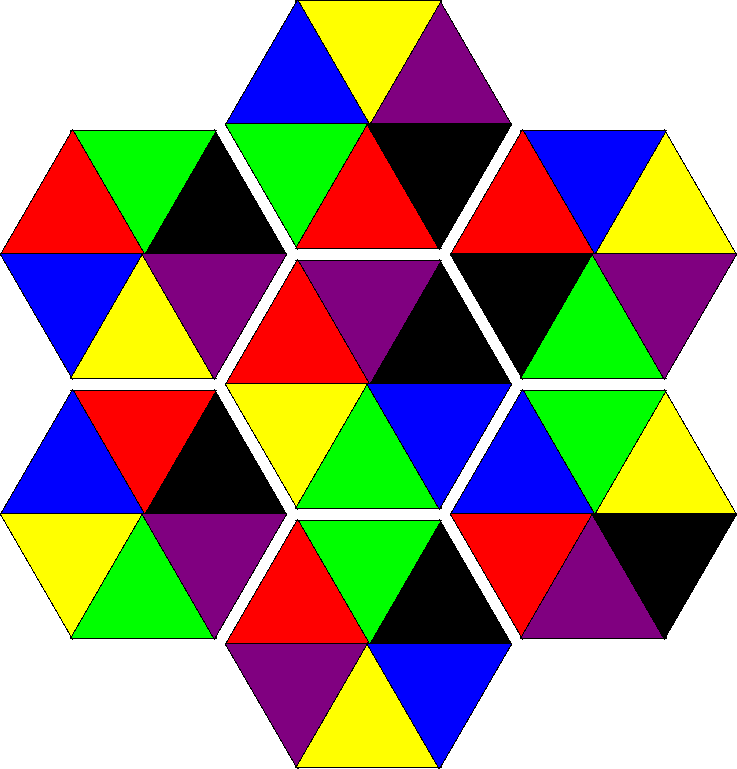
\includegraphics[width=.8\textwidth]{images/hexagons.pdf}
\end{center}

Ahhoz, hogy megoldjuk ezt a feladatot, először
valahogy le kell írnunk az ismert tényeket -- tehát
itt azt, hogy milyen lapok léteznek. A lapok színeit
egy \pr{l} struktúrába fogjuk össze, és a következő
tényeket kapjuk:
\begin{program}
lap(l(fekete,lila,sárga,kék,zöld,piros)).
lap(l(fekete,zöld,piros,kék,sárga,lila)).
lap(l(fekete,zöld,lila,sárga,kék,piros)).
lap(l(fekete,lila,piros,sárga,zöld,kék)).
lap(l(fekete,piros,kék,sárga,zöld,lila)).
lap(l(fekete,sárga,zöld,kék,piros,lila)).
lap(l(fekete,zöld,piros,lila,sárga,kék)).
\end{program}

Így például végig tudunk menni a lapokon a
\begin{query}
?- lap(L).
\end{query}
kérdés segítségével.

A lapok tetszőlegesen elforgathatóak, tehát a forgatásukra is kell valami mód. Ehhez először egyezzünk meg abban, hogy pontosan milyen elhelyezést jelent a színeknek egy sorrendje:
\begin{center}
  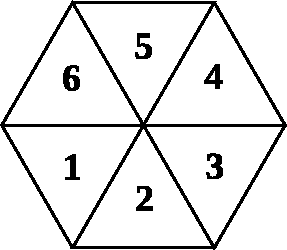
\includegraphics[width=.3\textwidth]{images/hexagon.pdf}
\end{center}

Tehát az első szín van délnyugatra, a második délre,
\dots a hatodik északnyugatra. Egy forgatás során
annyi történik, hogy valamelyik másik szín kerül
előre, de utána a sorrend változatlan. Ezt így
írhatjuk le:
\begin{program}
forgat(l(A,B,C,D,E,F), l(A,B,C,D,E,F)).
forgat(l(A,B,C,D,E,F), l(B,C,D,E,F,A)).
forgat(l(A,B,C,D,E,F), l(C,D,E,F,A,B)).
forgat(l(A,B,C,D,E,F), l(D,E,F,A,B,C)).
forgat(l(A,B,C,D,E,F), l(E,F,A,B,C,D)).
forgat(l(A,B,C,D,E,F), l(F,A,B,C,D,E)).
\end{program}

A következő feladat, hogy arra adjunk egy szabályt,
hogy mikor kapcsolódik helyesen két lap. Ehhez azt
is kell tudni, hogy egymáshoz képest hogyan
helyezkednek el. A \pr{kapcsolódik(L1, L2, Irány,
  F1, F2)} azt mondja, hogy ha az \pr{L1} laptól
\pr{Irány} irányba helyezzük le az \pr{L2} lapot,
akkor a két lap elforgatható egy \pr{F1} illetve
\pr{F2} helyzetbe úgy, hogy a találkozásuknál a
színek megegyeznek. Itt az irány leírására
használhatnánk a fent bevezetett számokat, de jobban
olvasható talán, ha égtájakat használunk. Nézzük meg
először a \pr{dny} (délnyugat) irányt!
\begin{program}
kapcsolódik(L1, L2, dny, F1, F2) :-
    forgat(L1, F1), forgat(L2, F2),
    F1 = l(X,_,_,_,_,_),
    F2 = l(_,_,_,X,_,_).
\end{program}
A törzs első sora csak annyit mond, hogy az \pr{F1}
és \pr{F2} az \pr{L1} és \pr{L2} elforgatottja; a
második és harmadik sor pedig azt biztosítja, hogy
az elforgatott lapokon a \emph{megfelelő} helyen
levő szín megegyezik (a többi nem számít). Mivel az
\pr{L1}-től délnyugatra van az \pr{L2}, ezért az
\pr{L1} délnyugati (első) színe az érdekes, az
\pr{L2}-nek pedig a szemben levő, tehát északkeleti
(negyedik) színe.

Teljesen hasonlóan felírhatjuk a többi égtájra is a
kapcsolódási szabályokat:
\begin{program}
kapcsolódik(L1, L2, d, F1, F2) :-
    forgat(L1, F1), forgat(L2, F2),
    F1 = l(_,X,_,_,_,_),
    F2 = l(_,_,_,_,X,_).
kapcsolódik(L1, L2, dk, F1, F2) :-
    forgat(L1, F1), forgat(L2, F2),
    F1 = l(_,_,X,_,_,_),
    F2 = l(_,_,_,_,_,X).
kapcsolódik(L1, L2, ék, F1, F2) :-
    forgat(L1, F1), forgat(L2, F2),
    F1 = l(_,_,_,X,_,_),
    F2 = l(X,_,_,_,_,_).
kapcsolódik(L1, L2, é, F1, F2) :-
    forgat(L1, F1), forgat(L2, F2),
    F1 = l(_,_,_,_,X,_),
    F2 = l(_,X,_,_,_,_).
kapcsolódik(L1, L2, ény, F1, F2) :-
    forgat(L1, F1), forgat(L2, F2),
    F1 = l(_,_,_,_,_,X),
    F2 = l(_,_,X,_,_,_).
\end{program}

Most már minden megvan ahhoz, hogy megkeressük a
megoldást. Ezt úgy találjuk meg, hogy veszünk 7
különböző (!) lapot, és felírjuk a rájuk vonatkozó
kapcsolódási feltételeket:
\begin{program}
megoldás(F1, F2, F3, F4, F5, F6, F7) :-
    lap(L1),
    lap(L2), L2 \= L1,
    lap(L3), L3 \= L1, L3 \= L2,
    lap(L4), L4 \= L1, L4 \= L2, L4 \= L3,
    lap(L5), L5 \= L1, L5 \= L2, L5 \= L3, L5 \= L4,
    lap(L6), L6 \= L1, L6 \= L2, L6 \= L3, L6 \= L4,
             L6 \= L5,
    lap(L7), L7 \= L1, L7 \= L2, L7 \= L3, L7 \= L4,
             L7 \= L5, L7 \= L6,
    kapcsolódik(L1, L2, dk,  F1, F2),
    kapcsolódik(F1, L7, ék,  F1, F7),
    kapcsolódik(F2, L3, ék,  F2, F3),
    kapcsolódik(F2, F7, é,   F2, F7),
    kapcsolódik(F3, L4, é,   F3, F4),
    kapcsolódik(F3, F7, ény, F3, F7),
    kapcsolódik(F4, L5, ény, F4, F5),
    kapcsolódik(F4, F7, dny, F4, F7),
    kapcsolódik(F5, L6, dny, F5, F6),
    kapcsolódik(F5, F7, d,   F5, F7),
    kapcsolódik(F6, F1, d,   F6, F1),
    kapcsolódik(F6, F7, dk,  F6, F7).
\end{program}
Itt a lapok számozása szintén a fenti módon
történik, a 7-es számú a középső lap. Az első hét
sor csak felveszi a lapokat, és biztosítja, hogy
mindegyik különböző legyen. Utána jönnek a szabályok
-- itt egy dologra kell figyelni, hogy (a
procedurális olvasat értelmében) a \pr{kapcsolódik}
szabályok kielégítése sorrendben történik, ezért
amint egy lapot ,,letettünk'', annak meghatározódik
a forgatása, tehát onnantól kezdve a forgatás
nélküli \pr{L} helyett az elforgatott \pr{F}-et kell
használni. Ezzel megköveteljük, hogy a
\pr{kapcsolódik}ban a ,,sima'' és ,,elforgatott''
változat megegyezzen, tehát ne tudja tovább forgatni
a lapot.

Keressük meg akkor a megoldást!
\begin{query}
?- megoldás(F1, F2, F3, F4, F5, F6, F7).
F1 = l(kék, zöld, piros, fekete, lila, sárga),
F2 = l(kék, sárga, lila, fekete, zöld, piros),
F3 = l(fekete, piros, kék, sárga, zöld, lila),
F4 = l(sárga, zöld, kék, piros, lila, fekete),
F5 = l(sárga, kék, fekete, zöld, piros, lila),
F6 = l(fekete, lila, piros, sárga, zöld, kék),
F7 = l(fekete, zöld, lila, sárga, kék, piros)
\end{query}

Ebben a programban rengeteg az ismétlés, ami nem túl
szép, de a jelenlegi eszközeinkből ennyire
futja. Nemsokára megismerkedünk a listákkal és a
számolással, amelyek segítségével a \pr{forgat} és a
\pr{kapcsolódik} szabályokat egy--egy sorban meg
lehetne oldani, és a \emph{megoldás}ban a lapok
különbözőségét is könnyebben lehetne biztosítani.

% -*- fill-column: 52 -*-
% (local-set-key (kbd "C-c C-f") 'display-fill-column-indicator-mode)
\chapter{Listák}
Ebben a leckében ...
\section{Listák}
Ahogy a múltkor láttuk, egy Prolog kifejezés vagy
egyszerű (konstans vagy változó), vagy egy fix
aritású összetett struktúra. Gyakran előfordul
azonban, hogy nem tudjuk előre, hogy hány adattal
akarunk foglalkozni. Hogyan tudnánk dolgoknak egy
listáját egy struktúrával kifejezni? Természetesen
rekurzívan! Kezdjük először csak két dologgal:
\index{lista}
\begin{query}
lista(a, b)
\end{query}
Ha hármat akarunk beletenni egy listába, akkor
megtehetnénk, hogy eggyel több argumentumot veszünk
bele:
\begin{query}
lista(a, b, c)
\end{query}
\dots de ez több okból sem igazán jó
megoldás. Egyrészt ez így egy másik funktor lesz
(hiszen más az aritása), másrészt ezzel még mindig
csak \emph{ismert} hosszúságú listákat tudnánk
készíteni. Helyette csinálhatjuk viszont a
következőt:
\begin{query}
lista(a, lista(b, c))
\end{query}
Ezt tetszőlegesen lehet folytatni, pl.
\begin{query}
lista(a, lista(b, lista(c, lista(d, e))))
\end{query}
Ez egyrészt azért jó, mert így mindig egy 2-aritású
\pr{lista} funktorunk van, másrészt ezzel tudunk
olyat írni, hogy
\begin{query}
lista(a, Maradék)
\end{query}
ami egy tetszőleges lista, aminek az első eleme
\pr{a}, vagy
\begin{query}
lista(a, lista(b, Maradék))
\end{query}
ami egy olyan tetszőleges lista, aminek az első két
eleme \pr{a} és \pr{b}.

Ennek így egy szépséghibája van: az utolsó elem
kezelése kicsit más, mint a többié, és emiatt pl.~az
előző példákban a ,,tetszőleges'' lista mégsem
teljesen tetszőleges, mert nem lehet egy-
ill.~kételemű. Ezt azzal tudjuk megoldani, hogy
bevezetünk egy olyan konstanst, amivel a lista végét
jelöljük. Pl.~az \pr{a}, \pr{b} és \pr{c} elemeket
tartalmazó lista ekkor így néz ki:
\begin{query}
lista(a, lista(b, lista(c, vége)))
\end{query}

A szokásos Prolog jelölés a \pr{lista} helyett a
pont (\pr{.}) funktor, a \pr{vége} helyett pedig a
szögletes zárójelpár (\pr{[]}) atom.\footnote{Az
\name{SWI-Prolog} a pontot lecserélte a kicsit
furcsán kinéző \pr{'[|]'} funktorra.}
Az előző listát tehát erre átírva ilyet kapunk:
\index{\pr{.}}\index{\pr{[]}}
\begin{query}
.(a, .(b, .(c, [])))
\end{query}
Ez sajnos nem a legkönnyebben olvasható. Szerencsére
van rá egy egyszerűsített jelölés:
\begin{query}
?- .(X, Y) = [X|Y].
true
\end{query}
Sőt, nem csak
\begin{query}
?- .(a, .(b, .(c, []))) = [a | [b | [c | []]]].
true
\end{query}
teljesül, hanem az egymásba ágyazást vesszővel lehet
helyettesíteni:
\begin{query}
?- [a | [b | [c | []]]] = [a, b, c | []].
true
\end{query}
És végül van még egy utolsó ,,egyszerűsítés'' (a
szakszó erre a \emph{szintaktikus cukor}): ha a
függőleges vonal jobboldalán a \pr{[]} van, akkor
ezt el lehet hagyni:
\index{szintaktikus cukor}
\begin{query}
?- [a, b, c | []] = [a, b, c].
true
\end{query}
Ez tehát a Prolog \emph{láncolt lista} struktúrája;
a \pr{[]} neve \emph{üres lista}, és egy \pr{[X|Y]}
listában az \pr{X} a lista \emph{eleje}, az \pr{Y}
pedig a lista \emph{maradéka}. A maradék mindig vagy
egy lista, vagy az üres lista atom.
\index{lista!láncolt}\index{lista!üres}
\index{lista!feje}\index{lista!maradéka}

A gyakorlatban mindig ezt az egyszerű formát
használjuk, de fontos érteni, hogy ez valójában
egymásba ágyazott funktorokból áll, és ezért
pl.~\pr{[a, b, c] = [a | [b, c]] = [a, b | [c]] =
  [a, b, c | []]}.

\section{Műveletek listákon}

Az alábbiakban nézzünk meg néhány hasznos műveletet,
amiket listákra alkalmazhatunk.

\subsection*{Tartalmazás}
Az egyik legfontosabb kérdés, amit listákkal
kapcsolatban feltehetünk, az az, hogy valami benne
van-e:
\begin{program}
tartalmaz(X, [X|_]).
tartalmaz(X, [_|Maradék]) :- tartalmaz(X, Maradék).
\end{program}
\index{\pr{tartalmaz}}
Szavakban megfogalmazva, egy lista akkor tartalmaz
valamit, (i) ha az az eleje, vagy (ii) ha a maradéka
tartalmazza azt. Ezzel
\begin{query}
?- tartalmaz(b, [a,b,c]).
true
?- tartalmaz(b, [a,[b,c]]).
false
?- tartalmaz([b,c], [a,[b,c]]).
true
\end{query}
Emellett a
\begin{query}
?- tartalmaz(X, [a,b,c]).
\end{query}
kérdésre megkapjuk az \pr{X = a}, \pr{X = b} és
\pr{X = c} megoldásokat, sőt, meg is fordíthatjuk,
és feltehetjük a kérdést, hogy ,,Milyen listák
tartalmazzák \pr{a}-t?''
\begin{query}
?- tartalmaz(a, L).
\end{query}
Erre a következő (jellegű) megoldásokat kapjuk:
\begin{query}
L = [a | Maradék]
L = [X, a | Maradék]
L = [X1, X2, a | Maradék]
L = [X1, X2, X3, a | Maradék]
...
\end{query}
Az első egy tetszőleges lista, aminek az első eleme
\pr{a}; a második egy olyan, aminek a második eleme
\pr{a} és így tovább.

Feltehetünk összetett kérdéseket is, pl.~milyen
háromelemű listák vannak, amelyek tartalmazzák az
\pr{a}, \pr{b} és \pr{c} elemeket?
\begin{query}
?- L = [_, _, _], tartalmaz(a, L),
   tartalmaz(b, L), tartalmaz(c, L).
L = [a, b, c]
L = [a, c, b]
L = [b, a, c]
L = [c, a, b]
L = [b, c, a]
L = [c, b, a]
\end{query}

\subsection*{Összefűzés}
Két listát össze is tudunk csatolni. Legyen
\pr{hozzáfűz(L1, L2, L3)} igaz akkor, ha \pr{L1} és
\pr{L2} egymás után rakva \pr{L3}-at adja, pl.
\begin{query}
?- hozzáfűz([a,b,c], [d,e], [a,b,c,d,e]).
true
\end{query}
Ha \pr{L1} üres, akkor \pr{L2} és \pr{L3}
megegyezik:
\begin{program}
hozzáfűz([], L2, L2).
\end{program}
Egyébként \pr{L1} első eleme az \pr{L3} első eleme
lesz; az \pr{L3} maradéka pedig az \pr{L1}
maradékának és az \pr{L2}-nek az összefűzéséből
adódik:
\begin{program}
hozzáfűz([X|M1], L2, [X|M3]) :- hozzáfűz(M1, L2, M3).
\end{program}
\index{\pr{hozzáfűz}}

Annak ellenére, hogy onnan indultunk, hogy hogyan
lehet két listát összefűzni, a kérdés ismét
megfordítható, pl.~,,Hogyan lehet egy listát két
listára osztani?''
\begin{query}
?- hozzáfűz(L1, L2, [a,b,c]).
L1 = [],
L2 = [a, b, c]
L1 = [a],
L2 = [b, c]
L1 = [a, b],
L2 = [c]
L1 = [a, b, c],
L2 = []
\end{query}

Vagy: ,,Igaz-e, hogy az \pr{[a,b]} listával kezdődik
az \pr{[a,b,c]} lista?''
\begin{query}
?- hozzáfűz([a,b], _, [a,b,c]).
true
\end{query}

Megkereshetjük vele egy listában az előző és
következő elemet:
\begin{query}
?- hozzáfűz(_, [Előző, már, Következő | _],
   [jan, feb, már, ápr, máj, jún,
    júl, aug, szep, okt, nov, dec]).
Előző = feb,
Következő = ápr
\end{query}

A \pr{tartalmaz} szabályt is leírhatjuk a
segítségével:
\begin{program}
tartalmaz(X, L) :- hozzáfűz(_, [X|_], L).
\end{program}
Szavakban: egy \pr{L} lista akkor tartalmaz egy
\pr{X} elemet, ha szétválasztható két listára,
amiből a másodiknak az első eleme \pr{X}. (Az első
lista ill.~a második maradéka is lehet üres.)

\subsection*{Hozzáadás és törlés}
Új elemet egy lista elejéhez olyan könnyű hozzáadni,
hogy erre nem is szokás külön szabályt írni, de ha
akarunk, itt van:
\begin{program}
hozzáad(X, L, [X|L]).
\end{program}
A listák végére (hatékonyan!) beszúrni kicsit
bonyolultabb, majd később lesz róla szó.

Hogyan kell törölni egy elem egy előfordulását egy
listából?
\begin{program}
töröl(X, [X|M], M).
töröl(X, [Y|M], [Y|M1]) :- töröl(X, M, M1).
\end{program}
\index{\pr{töröl}}
Tehát: ha \pr{X} a lista első eleme, akkor a törlés
után a lista maradékát kapjuk. Egyébként a lista
első eleme és az eredmény első eleme megegyezik, és
az eredmény maradéka pedig ugyanaz, mint az eredeti
lista maradéka, amiből kitöröltük az \pr{X}-et.

Egy példa a használatára:
\begin{query}
?- töröl(a, [a,b,a,a], L).
L = [b, a, a]
L = [a, b, a]
L = [a, b, a]
\end{query}
Itt a második és harmadik megoldás azonosnak tűnik,
de valójában az egyik az eredeti listából az \pr{a}
elem második, a másik pedig a harmadik előfordulását
törölte.

Mi történik, ha az ,,eredeti'' listát vesszük
ismeretlennek?
\begin{query}
?- töröl(a, L, [1,2,3]).
L = [a, 1, 2, 3]
L = [1, a, 2, 3]
L = [1, 2, a, 3]
L = [1, 2, 3, a]
\end{query}
Ahogy látszik, a ,,Mi az a lista, amiből ha
kitörlünk egy \pr{a}-t, akkor \pr{[1,2,3]}-at
kapunk?'' kérdés egyszerűbben úgy fogalmazható meg,
hogy ,,Mit kapunk, ha az \pr{[1, 2, 3]} listába
beleteszünk egy \pr{a}-t?''

Ez van annyira hasznos, hogy adhatunk neki egy új
nevet:
\begin{program}
betesz(X, L, L1) :- töröl(X, L1, L).
\end{program}
\index{\pr{betesz}}

A törlés használható kiválasztásra is:
\begin{query}
?- töröl(X, [a,b,c], _).
X = a
X = b
X = c
\end{query}

Ha a törölni kívánt elem nem szerepel a listában, az
eredmény \pr{false} lesz. Ezt kihasználva ezzel is
definiálhatjuk a \pr{tartalmaz} szabályt:
\begin{program}
tartalmaz(X, L) :- töröl(X, L, _).
\end{program}

\subsection*{Részlisták}
Következőnek nézzük meg, hogy mikor része egy lista
egy másiknak:
\begin{query}
?- részlista([c,d,e], [a,b,c,d,e,f]).
true
?- részlista([c,e], [a,b,c,d,e,f]).
false
\end{query}
\index{\pr{részlista}}

Ahogy a második példából látszik, itt a ,,részét''
nem úgy értelmezzük, hogy az első lista minden
elemét tartalmazza a második (mint egy halmaznál),
hanem hogy pontosan ugyanolyan sorrendben, más
elemek közbeékelődése nélkül szerepelnek.

Ez a szabály könnyen megadható a \pr{hozzáfűz}
segítségével:
\begin{program}
részlista(R, L) :-
    hozzáfűz(_, L1, L), hozzáfűz(R, _, L1).
\end{program}
Tehát \pr{R} akkor része \pr{L}-nek, ha valamilyen
listát elé- és utánafűzve megkapjuk \pr{L}-et. A
definíció ezt két részletben írja le: az első tag
azt mondja, hogy az \pr{L} az \pr{L1} listára
végződik; a második pedig azt, hogy ez az \pr{L1}
lista az \pr{R}-el kezdődik. A vég kezdete pedig épp
azt jelenti, hogy \pr{R} valahol belül van
\pr{L}-ben (vagy valamelyik szélén, ha az itt
alsóvonással jelölt listák egyike az üres lista).

Szokás szerint nézzük meg, mit kapunk a
,,fordított'' felhasználásban:
\begin{query}
?- részlista(R, [a,b,c]).
R = []
R = [a]
R = [a, b]
R = [a, b, c]
R = []
R = [b]
R = [b, c]
R = []
R = [c]
R = []
\end{query}
Ahogy várható volt, ezzel megkapjuk az \pr{[a,b,c]}
lista összes részlistáját -- az üreset többször is
(miért? Tipp: nézd meg a \pr{hozzáfűz(X, \_,
  [a,b,c])} kimenetét).

\subsection*{Permutációk}
Két lista akkor \emph{permutációja} vagy átrendezése
egymásnak, ha ugyanazokat az elemeket
tartalmazzák. Az üres listának csak az üres lista a
permutációja:
\begin{program}
permutáció([], []).
\end{program}
Ha az első lista nem üres, akkor visszavezethetjük a
feladatot az eggyel rövidebb listákra:
\begin{program}
permutáció([X|M], P) :-
    permutáció(M, L), betesz(X, L, P).
\end{program}
\index{\pr{permutáció}}
Tehát úgy kapjuk az első lista permutációját, hogy
vesszük a maradék (\pr{M}) egy permutációját
(\pr{L}), és ebbe betesszük az \pr{X}-et.

Egy másik logika az lehet, hogy kiválasztunk
(kitörlünk) egy elemet, a maradéknak vesszük egy
permutációját, és az elejáre beszúrjuk a kitörölt
elemet:
\begin{program}
permutáció(L, [X|P]) :-
    töröl(X, L, M), permutáció(M, P).
\end{program}

Ellenőrizzük, hogy működik-e! A
\begin{query}
?- permutáció([piros, zöld, kék], P).
\end{query}
kérdésre mindkettő visszaadja mind a 6 jó megoldást
(bár különböző sorrendben) és közli, hogy nincs
több. Viszont a fordított
\begin{query}
?- permutáció(P, [piros, zöld, kék]).
\end{query}
esetben az első verzió a 6 megoldás után végtelen
rekurzióba kerül, a másodiknál pedig már az első
után beragad. Meg lehet oldani, hogy mindig jó
legyen, csak kicsit ki kell egészíteni, de mivel
szimmetrikus, nincs rá igazán szükség.

\begin{problem}
Írjatok egy szabályt, amivel ki lehet venni egy
listából az utolsó 3 elemet!
\begin{query}
?- kivesz3([a,b,c,d,e], [a,b]).
true
\end{query}
\end{problem}
\begin{problem}
Írjatok egy szabályt, amivel ki lehet venni egy
listából az első és utolsó 3 elemet!
\begin{query}
?- kivesz33([a,b,c,d,e,f,g], [d]).
true
\end{query}
\end{problem}
\begin{problem}
Írjatok egy szabályt, amivel megkaphatjuk egy lista
utolsó elemét! Készítsetek két verziót, egyet
\pr{hozzáfűz}zel, egyet anélkül!
\begin{query}
?- utolsó([a,b,c], c).
true
\end{query}
\end{problem}
\begin{problem}
Írjátok meg a \pr{páros\_hosszú(L)} és
\pr{páratlan\_hosszú(L)} szabályokat! Ezek akkor
igazak, amikor az \pr{L} lista páros- ill.~páratlan
számú elemből áll (nincs szükség számokra hozzá).
\end{problem}
\begin{problem}
Írjatok egy szabályt, ami megállapítja, hogy két
lista megfordítottja-e egymásnak!
\begin{query}
?- fordított([a,b,c], X).
X = [c,b,a]
\end{query}
\end{problem}
\begin{problem}
Írjatok egy szabályt, ami megállapítja, hogy egy szó
\emph{palindróma}-e, azaz visszafele is ugyanaz-e!
\begin{query}
?- palindróma([g,ö,r,ö,g]).
true
\end{query}
\end{problem}
\begin{problem}
Írjatok egy szabályt, amivel egy listát eggyel
,,elforgathatunk'' úgy, hogy az első lista első eleme
a második végére kerül!
\begin{query}
?- forgat([a, b, c, d], [b, c, d, a]).
true
\end{query}
\end{problem}
\begin{problem}
Írjatok egy szabályt, ami a részhalmazságot
vizsgálja! Le is lehessen vele generálni az összes
részhalmazt! (A halmaz itt egy olyan rendezett
lista, amiben minden elem egyszer fordul elő.)
\begin{query}
?- részhalmaz([a, b, c], R).
R = [a, b, c]
R = [a, b]
R = [a, c]
R = [a]
R = [b, c]
R = [b]
R = [c]
R = []
\end{query}
(Az eredmény lehet más sorrendben.)
\end{problem}
\begin{problem}
Írjatok egy szabályt, amivel ellenőrizhető, hogy két
lista ugyanolyan hosszú!
\begin{query}
?- ugyanolyan_hosszú([1, 2, 3], [a, b, c]).
true
\end{query}
\end{problem}
\begin{problem}
Írjatok egy szabályt, amivel ki lehet ,,lapítani''
egy listát, tehát a belső listák elemeit kiviszi a
legkülső szintre:
\begin{query}
?- lapít([a, b, [c, d], [], [[[e]]], f], L).
L = [a, b, c, d, e, f]
\end{query}
\end{problem}
\section{Projekt: Dobble Kids}
A Dobble Kids társasjáték 30 kártyából áll, ahol
minden kártyán 6 különböző állat szerepel (összesen
31 fajtából), amelyekre az az érdekes tulajdonság
teljesül, hogy bármely két lapon pontosan egy azonos
állat van.
\begin{figure}[ht]
\begin{center}
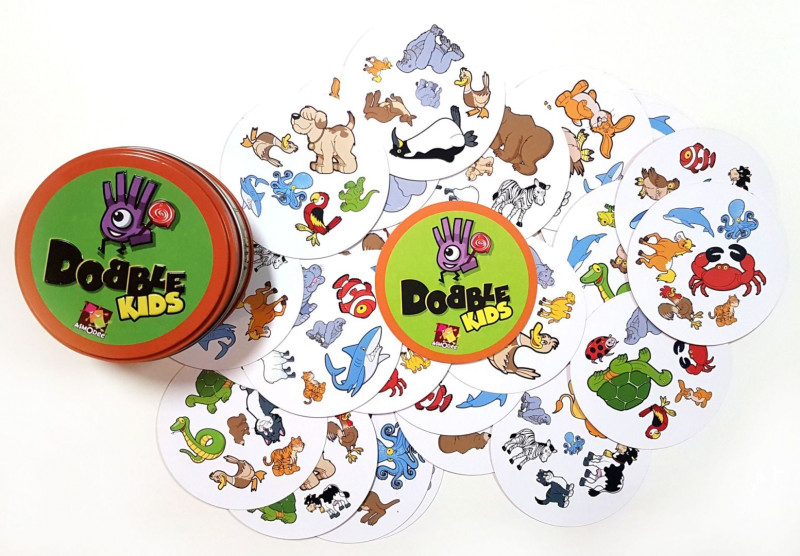
\includegraphics[width=\textwidth]{images/dobble-kids.jpg}
\end{center}
\end{figure}
Egy ilyen kártyapakli generálása nem könnyű feladat,
és nagyon szép matematika van a hátterében. Meg
lehet mutatni, hogy ha egy lapon $k$ állat van,
akkor összesen $k(k-1)+1$ különböző kártya
készíthető. Viszont $k = 6$ esetén ez 31, nem 30,
tehát van egy olyan lap, amit még hozzá lehetne
venni a paklihoz, hogy a tulajdonság továbbra is
fennálljon. Keressük meg ezt a lapot!

Először is készítsük el a pakliban levő kártyák
listáját! Minden kártya állatok listája, tehát a
pakli listák listája lesz:
\begin{program}
lapok([[bagoly,bálna,hal,kacsa,rák,tehén],
       [bagoly,bárány,elefánt,polip,teknős,teve],
       [bagoly,béka,delfin,gorilla,kígyó,kutya],
       [bagoly,cápa,cica,kakas,nyuszi,pingvin],
       [bagoly,katica,kenguru,krokodil,tigris,zebra],
       [bagoly,ló,medve,oroszlán,papagáj,víziló],
       [bálna,bárány,cica,delfin,kenguru,papagáj],
       [bálna,béka,cápa,ló,teknős,zebra],
       [bálna,elefánt,kutya,nyuszi,oroszlán,tigris],
       [bálna,gorilla,kakas,krokodil,medve,teve],
       [bálna,katica,kígyó,pingvin,polip,víziló],
       [bárány,béka,kacsa,kakas,katica,oroszlán],
       [bárány,cápa,gorilla,hal,tigris,víziló],
       [bárány,kígyó,krokodil,ló,nyuszi,tehén],
       [bárány,kutya,medve,pingvin,rák,zebra],
       [béka,cica,elefánt,krokodil,rák,víziló],
       [béka,hal,kenguru,medve,nyuszi,polip],
       [béka,papagáj,pingvin,tehén,teve,tigris],
       [cápa,delfin,elefánt,katica,medve,tehén],
       [cápa,kacsa,krokodil,kutya,papagáj,polip],
       [cápa,kenguru,kígyó,oroszlán,rák,teve],
       [cica,gorilla,oroszlán,polip,tehén,zebra],
       [cica,kacsa,kígyó,medve,teknős,tigris],
       [delfin,hal,krokodil,oroszlán,pingvin,teknős],
       [delfin,kacsa,nyuszi,teve,víziló,zebra],
       [delfin,kakas,ló,polip,rák,tigris],
       [elefánt,gorilla,kacsa,kenguru,ló,pingvin],
       [elefánt,hal,kakas,kígyó,papagáj,zebra],
       [gorilla,katica,nyuszi,papagáj,rák,teknős],
       [kakas,kenguru,kutya,tehén,teknős,víziló]]).
\end{program}

Szintén hasznos lehet az összes állat listája:
\begin{program}
állatok([bagoly,bálna,bárány,béka,cápa,cica,delfin,
         elefánt,gorilla,hal,kacsa,kakas,katica,
         kenguru,kígyó,krokodil,kutya,ló,medve,
         nyuszi,oroszlán,papagáj,pingvin,polip,rák,
         tehén,teknős,teve,tigris,víziló,zebra]).
\end{program}

Ha most ezekből az állatokból egy kártyát szeretnék
képezni, akkor annak két dolgot kell teljesítenie:
(i) 6 elemből kell állnia, és (ii) az állat-lista
részhalmazának kell lennie. Az alábbi szabály az
\pr{A} listából választ ki 6 különböző elemet:
\begin{program}
választ6(A, L) :-
    L = [_, _, _, _, _, _],
    részhalmaz(A, L).
\end{program}

A \pr{részhalmaz} szabály feladatként fel volt adva;
az alábbi verzió feltételezi, hogy az elemek azonos
sorrendben fordulnak elő (tehát nincs olyan elempár,
ami a két listában fordított sorrendben
szerepelne). Ez a megkötés, mivel most úgy
használjuk, hogy a részhalmaz elemei változók, azt
vonja maga után, hogy a keletkező részhalmazban az
elemek olyan sorrendben lesznek, mint ahogy a
teljesben szerepeltek.
\begin{program}
részhalmaz([], []).
részhalmaz([X|M], [X|R]) :- részhalmaz(M, R).
részhalmaz([_|M], R) :- részhalmaz(M, R).
\end{program}
\index{\pr{részhalmaz}}
Az üres halmaznak csak az üres halmaz a
részhalmaza. Egyébként úgy kapunk meg egy
részhalmazt, hogy az első elemet (\pr{X}) vagy
hozzáadjuk (2.~sor), vagy nem adjuk hozzá (3.~sor) a
maradék (\pr{M}) egy részhalmazához (\pr{R}).

A következő feladatunk, hogy ha készítettünk egy
lapot, akkor eldöntsük, hogy jó-e. Ezt úgy tudjuk
megtenni, hogy összehasonlítjuk a többi lappal
egyenként, és megnézzük, hogy az állat-halmazok
metszete 1-elemű-e:
\begin{program}
jó_lap([], _).
jó_lap([L|M], X) :- metszet(X, L, [_]), jó_lap(M, X).
\end{program}
Itt az első argumentum a többi kártya listája; ha ez
üres, az azt jelenti, hogy minden kártyát
leteszteltünk, készen vagyunk. Egyébként megnézzük,
hogy az aktuális kártyára a metszet 1-elemű-e (hogy
mi ez az elem, az nem érdekes), és még ellenőrizni
kell a maradékra is.

A metszet számítása van még hátra:
\begin{program}
metszet([], _, []).
metszet([X|L1], L2, [X|L3]) :-
    tartalmaz(X, L2), metszet(L1, L2, L3).
metszet([X|L1], L2, L3) :-
    nemtartalmaz(X, L2), metszet(L1, L2, L3).
\end{program}
Az üres halmaz metszete bármivel üres. Ha az első
elem (\pr{X}) szerepel a másik halmazban (\pr{L2}),
akkor benne lesz a metszetben is; különben nem.

Azt, hogy egy elem \emph{nincs benne} egy listában,
a \pr{nemtartalmaz} fejezi ki:
\begin{program}
nemtartalmaz(_, []).
nemtartalmaz(X, [Y|M]) :- X \= Y, nemtartalmaz(X, M).
\end{program}

Ezzel minden megvan már, csak össze kell rakni a
darabokat:
\begin{program}
megoldás(X) :-
    állatok(A), lapok(L),
    választ6(A, X), jó_lap(L, X).
\end{program}
Röviden: kiválasztunk 6 állatot úgy, hogy az így
készült kártya jó legyen a pakli minden lapjához.

Ha kipróbáljuk, kicsit hosszabb gondolkodás után
megkapjuk a megoldást:
\begin{query}
?- megoldás(X).
X = [cica, hal, katica, kutya, ló, teve]
\end{query}

Ezen a programon is sokat tudunk majd
javítani. Magasabb rendű szabályokkal kényelmesen le
lehet generálni az \pr{állatok} listát, és nem kell
kézzel megadni; valamint a \pr{nemtartalmaz}ra nem
lesz szükség, ha megtanuljuk a \emph{vágásokat}.

% -*- fill-column: 52 -*-
% (local-set-key (kbd "C-c C-f") 'display-fill-column-indicator-mode)
\chapter{Operátorok}
Van még szintaktikus cukor bizonyos struktúrákon:
ezek az \emph{operátorok}. Amikor például leírunk
egy olyan matematikai kifejezést, hogy $2a+bc$, vagy
a szorzásokat csillaggal (\pr{*}) jelölve,
\pr{2*a+b*c}, akkor a szorzás és összeadás műveletek
az argumentumaik \emph{között} szerepelnek. Ezeket
hívjuk \emph{infix} (,,közbülső'') operátoroknak. Ha
egy ilyen kifejezést a szokásos \emph{prefix}
(,,elülső'') funktorokkal szeretnénk leírni, akkor
ezt kapnánk:
\index{operátor}
\index{operátor!prefix}
\index{operátor!infix}
\begin{query}
+(*(2, a), *(b, c))
\end{query}
Vannak nyelvek, amelyek ezt preferálják, és vannak
olyanok, amelyek a \emph{posztfix} (,,hátulsó'')
operátorokat:
\index{operátor!posztfix}
\begin{query}
((2, a)*, (b, c)*)+
\end{query}
... de a Prolog ezekre a megszokott infix
jelöléseket támogatja.

\begin{infobox*}{}{pre-, in- és posztfix}
Kizárólag prefix operátorokkal működnek a
\emph{Lisp} nyelvcsalád nyelvei (Common Lisp,
Scheme, Clojure, Racket etc.) Ezeknél a funktor neve
is a zárójelen belülre kerül, tehát a fenti példából
ez lesz: {\tt (+ (* 2 a) (* b c))}
\index{Lisp}

Ennek az egyik előnye a következetesség, a másik
pedig, hogy a műveletek kiterjeszthetőek több
argumentumra. Lispben például értelmes a {\tt (+ 1 2
  3 4 5)} kifejezés, amelynek értéke 15.

Kizárólag posztfix operátorokkal működnek a
\emph{veremnyelvek}, mint pl.~a Forth vagy a
PostScript. Itt minden operátornak csak egyféle
aritása lehet, de cserébe megszabadulunk a
zárójelektől. A fenti példa Forthban: {\tt 2 a * b c
  * +} \index{Forth}\index{veremnyelv}

Ezt hívják \emph{Reverse Polish Notation}-nek (RPN,
,,fordított lengyel jelölés''). Sok számológép is
használja; elsőre elég furcsa, de nagyon kényelmes és gyors,
ha megszokjuk.
\index{RPN}
\end{infobox*}

Tetszőleges funktorból lehet operátort csinálni. Az
egyargumentumú funktorok lehetnek pre- vagy
posztfixek, a kétargumentumúak pedig csak
infixek. Ahhoz, hogy egy ilyen kifejezést értelmezni
lehessen, még azt is kell tudni, hogy melyik operátornak
van elsőbbsége -- például a szorzást előbb kell
elvégezni, mint az összeadást, tehát elsőbbsége van.
\index{elsőbbség}

A Prologban az ilyen jellegű ,,beállításokat'' olyan
szabályokkal lehet megadni, amelyeknek nincsen feje,
csak törzse. Néhány példa operátorok definíciójára
(ezek részei az alapbeállításnak):
\begin{program}
:- op(200, fy, -).
:- op(400, yfx, *).
:- op(500, yfx, +).
:- op(1000, xfy, ',').
:- op(1200, xfx, :-).
\end{program}
Itt az első, 1 és 1200 közti szám adja meg a
\emph{precedenciá}\/t (minél kisebb, annál korábban
kell elvégezni az adott műveletet), a második a
típusát, és a harmadik magát az operátort.
\index{precedencia}

Hétféle típus létezik:
\begin{itemize}
\item \pr{xfx}, \pr{xfy}, \pr{yfx}: infix operátorok
\item \pr{fx}, \pr{fy}: prefix operátorok
\item \pr{xf}, \pr{yf}: posztfix operátorok
\end{itemize}

Ezeket úgy kell értelmezni, hogy az \pr{f} mutatja
az operátor helyét, az \pr{x} és \pr{y} pedig az
argumentumo(ka)t. Ha egy argumentum \pr{x}-el van
jelölve, akkor -- amennyiben az is egy operátoros
kifejezés -- az \pr{x} operátorának szigorúan kisebb
precedenciájúnak kell lennie az \pr{f}-nél. Ezzel
szemben az \pr{y} esetében ez nem csak kisebb lehet,
hanem egyenlő is. A zárójelezés minden előtt
elsőbbséget élvez (0 a precedenciája).

Nézzünk ez alapján egy pár példát arra, hogy a
Prolog különböző kifejezéseket hogyan elemez:
\begin{enumerate}
\item Mivel a \pr{+} operátor \pr{yfx} típusú, ha
  egy \pr{a + b + c} kifejezésem van, akkor ezt nem
  értelmezhetem úgy, hogy \pr{+(a, +(b, c))}, mert
  akkor a külső \pr{+} második argumentumában levő
  \pr{+(b, c)} kifejezés precedenciája megegyezik a
  \pr{+}-éval (hiszen az is \pr{+}). Viszont ha
  \pr{+(+(a, b), c)} módon értelmezem, ez a probléma
  nem lép fel: az első argumentumban levő \pr{+(a,
    b)} kifejezés precedenciája ugyan ugyanaz, de ez
  megengedett, mert a baloldali egy
  \pr{y}-argumentum. Tehát az \pr{yfx} operátorokat
  {\bf balról jobbra} kell zárójelezni.
\item A \pr{-a * (b + c * d)} kiértékelését először
  a zárójeles rész-szel kell kezdeni. Ezt nem
  értelmezhetem úgy, hogy \pr{*(+(b, c), d)}, mivel
  a \pr{+} precedenciája nagyobb a \pr{*}-énál, az
  \pr{yfx} szerint pedig kisebbnek vagy egyenlőnek
  kéne lennie. Ezért a helyes értelmezés a \pr{+(b,
    *(c, d))}. Ezután jön a 200-as precedenciájú
  1-argumentumú \pr{-} operátor, és végül a 400-as
  precedenciájú \pr{*}. A teljes kifejezés tehát így
  néz ki: \pr{*(-(a),+(b,*(c,d)))}.
\item A \pr{P :- Q, R, S} kifejezés helyes
  zárójelezése \pr{:-(P, ','(Q, ','(R, S)))}, mivel
  az \pr{xfy} típusú vessző operátort {\bf jobbról
  balra} kell zárójelezni, és a \pr{:-} operátor
  precedenciája a legmagasabb.
\item Mivel a \pr{:-} operátor \pr{xfx} típusú,
  ezért {\bf nem szerepelhet a saját
  argumentumaként}. Egy olyan kifejezésnek, hogy
  \pr{a :- b :- c}, nincsen helyes zárójelezése.
\item A negálás \pr{fy} típusú, ezért a \pr{- -a}
  kifejezés is elfogadható (a két mínuszjelet el
  kell választani, különben egy \pr{-{}-} nevű
  operátor lesz belőle); ha \pr{fx} típusú lenne,
  akkor ezt zárójelezni kéne \pr{-(-a)} alakban.
\end{enumerate}
A precedencia tehát többek közt azt is meghatározza,
hogy mi egy kifejezésben az elsődleges funktor,
ezért pl.
\begin{query}
?- X+Y = 2*3+5.
X = 2*3
Y = 5
?- X*Y = 2*3+5.
false
\end{query}

Nem csak különleges karakterekkel megadott
funktorokból készíthetünk operátorokat, hanem
tetszőleges nevűekből. Ez magyarul kevésbé
természetes, mint angolul, de azért nézzünk erre is
példát!
\begin{query}
:- op(600, xfx, benne_van).
X benne_van L :- tartalmaz(X, L).
\end{query}
Ez definiálja a \pr{tartalmaz} funktor infix
változatát. Ezután
\begin{query}
?- b benne_van [a, b, c].
true
?- benne_van(b, [a, b, c]).
true
\end{query}

\begin{infobox}{}{izoláló nyelvek}
A magyar nyelv ragozási rendszere mellett egy-egy
operátorrá tett szó magában még nem képes
természetes mondatok készítésére, de más nyelvekben
ez nagyon jól működik. Ezek az ún.~\emph{izoláló}
nyelvek -- jellemzően ilyenek a (dél)kelet-ázsiai
nyelvek, pl. kínai, indonéz vagy thai, de bizonyos
mértékig az angol is.
\end{infobox}

\begin{problem}
Mit ad az alábbi program:
\begin{query}
t(0+1, 1+0).
t(X+0+1, X+1+0).
t(X+1+1, Z) :- t(X+1, X1), t(X1+1, Z).
\end{query}
\dots a következő kérdésekre:
\begin{query}
?- t(0+1, A).
?- t(0+1+1, B).
?- t(1+0+1+1+1, C).
?- t(D, 1+1+1+0).
\end{query}
\end{problem}

\section{Számolás}
Ahogy az előző feladatban is látszott, a matematikai
kifejezések a Prolog számára csak struktúrák, és
ezért az
\begin{query}
?- X = 1 + 2.
\end{query}
kérdésre azt a (nem túl sokatmondó) választ kapjuk,
hogy
\begin{query}
X = 1 + 2
\end{query}

Ha rá akarjuk kényszeríteni, hogy kiértékelje a
kifejezést, az egyenlőség helyett az \pr{is}
operátort használhatjuk:
\begin{query}
?- X is 1 + 2.
X = 3
\end{query}

A matematikai kifejezésekben használható az
összeadás (\pr{+}), kivonás/negáció (\pr{-}),
szorzás (\pr{*}), osztás (\pr{/}), egészosztás
(\pr{//}), hatványozás (\pr{**}), és a
maradékszámítás (\pr{mod}). Néhány példa:
\begin{query}
?- X is 5/2.
X = 2.5
?- X is 9//2.
X = 4 % 9-ben 4-szer van meg (teljesen) a 2
?- X is 2**128.
X = 340282366920938463463374607431768211456.
?- X is 10 mod 3.
X = 1 % 10-nek a 3-mal vett osztási maradéka 1
\end{query}
\index{\pr{+}}\index{\pr{*}}\index{\pr{**}}
\index{\pr{-}}\index{\pr{/}}\index{\pr{//}}
\index{\pr{mod}}

Szintén alkalmazhatóak olyan gyakran használt
matematikai függvények, mint az abszolutérték
(\pr{abs}), a szinusz (\pr{sin}), vagy a természetes
alapú logaritmus (\pr{log}).
\index{\pr{abs}}\index{\pr{sin}}\index{\pr{log}}

A relációs jelek szintén ,,kiértékelő erővel''
bírnak, tehát pl.
\begin{query}
?- 2 + 2 > 3.
true
\end{query}
A nagyobb-egyenlő és kisebb-egyenlő relációk rendre
\pr{>=} és \pr{=<}, a matematikai egyenlőség és
különbözőség pedig \pr{=:=} és \pr{=\textbackslash=}, pl.
\index{\pr{>}}\index{\pr{<}}
\index{\pr{>=}}\index{\pr{=<}}
\index{\pr{=:=}}\index{\pr{=\textbackslash=}}
\begin{query}
?- 2 + 3 = 6 - 1.
false
?- 2 + 3 =:= 6 - 1.
true
?- 2 + 3 \= 6 - 1.
true
?- 2 + 3 =\= 6 - 1.
false
\end{query}

A matematikai kiértékelésnél feltétel, hogy a
kifejezésben ne szerepeljen változó. Tehát a
rendszer nem tudja azt megválaszolni, hogy:
\begin{query}
?- X + 2 < X + 3.
\end{query}
\dots bármennyire is nyilvánvalónak tűnik nekünk.

Az \pr{is} és az \pr{=:=} időnként ugyan
felcserélhető, de általában nem:
\begin{query}
X is 1 + 2.  % OK, X = 3
X =:= 1 + 2. % Nem jó, nem lehet benne ismeretlen
3 is 1 + 2.  % OK, baloldalt lehet szám
3 =:= 1 + 2. % OK
1 + 2 is 3.  % Nem jó, baloldalt nem lehet kifejezés
1 + 2 =:= 3. % OK
\end{query}

\subsection*{Legnagyobb közös osztó}

Két szám legnagyobb közös osztójának megkeresése
klasszikus probléma. Az alábbi megoldás ötlete
Euklidész \emph{Elemek} c. művéből származik
(i.e.~300 körül).
\index{algoritmus!euklidészi}

Legyen \pr{lnko(N, M, O)} igaz, ha \pr{N} és \pr{M}
legnagyobb közös osztója \pr{O}. Ha a két szám
azonos, akkor az osztó is az lesz:
\index{\pr{lnko}}
\begin{program}
lnko(N, N, N).
\end{program}
Ha az első szám a kisebb, akkor azt levonhatjuk a
másodikból, és a legnagyobb közös osztó nem
változik:
\begin{program}
lnko(N, M, O) :-
    N < M,
    M1 is M - N,
    lnko(N, M1, O).
\end{program}
Végül, ha a második szám a kisebb, akkor egyszerűen
cseréljük meg a két számot, és az előző esethez
jutunk:
\begin{program}
lnko(N, M, O) :-
    N > M,
    lnko(M, N, O).
\end{program}
Könnyen látszik, hogy a 3.~típusú lépés után mindig
2.~típusú jön, és a 2.~típusú lépés után az \pr{N +
  M} összeg csökken. Mivel a számok nem mehetnek 0
alá, előbb-utóbb biztosan eljut az 1.~típusú
lépéshez, ahol megkapjuk az eredményt.

Teszteljük!
\begin{query}
?- lnko(1071, 462, X).
X = 21.
\end{query}

A fenti magyarázatok deklaratív jellegűek. A
procedurális olvasata a programnak a következő:
\begin{enumerate}
\item Ha \pr{N = M}, akkor a legnagyobb közös osztó
  \pr{N}. Vége.
\item Ha \pr{N < M}, akkor vonjuk ki \pr{M}-ből
  \pr{N}-et, és menjünk vissza az 1.~lépésre.
\item Ha \pr{N > M}, akkor cseréljük meg \pr{N}-et
  és \pr{M}-et, és menjünk vissza az 1.~lépésre.
\end{enumerate}
Az ilyen megoldási módszereket \emph{algoritmusnak}
nevezik.\index{algoritmus}

\begin{infobox}{}{algoritmusok}
Bár Euklidész algoritmusa régi, de már sokkal
régebben is léteztek hasonló módszerek, pl.~az ókori
Mezopotámiában a sumérok már i.e.~2500 körül
ismertek algoritmust az osztásra. Maga az elnevezés
egy Bagdadban tanító VIII--IX.~századi perzsa
matematikus nevéből származik, akit (arabosan) úgy
hívtak, hogy Muhammad bin Múszá \emph{al-Khvárizmí}
(,,a Hvárezmből való Mózes fia Mohamed'').
\index{al-Khvárizmí}

Ha már a kezdeteknél tartunk, az első program, amelyet
tényleg számítógépre írtak, Ada Lovelace (1815--1852)
nevéhez fűződik, aki Byronnak, a híres költőnek
a lánya volt. A program a Bernoulli-számokat számította
ki; a gép pedig, amire írta, egy mechanikus
számítógép volt, a \emph{Difference Engine}. Ezt
Charles Babbage (1791--1871) tervezte, de csak
születésének 200 éves évfordulájára készült el
(viszont működött!).
\index{Ada Lovelace}\index{Babbage}
\end{infobox}

\subsection*{Listák hossza}
Most, hogy már tudunk számolni, ki tudjuk számítani
egy lista hosszát is:
\begin{program}
hossz([], 0).
hossz([_|M], N) :- hossz(M, N1), N is 1 + N1.
\end{program}
Egy üres lista hossza 0, egyébként meg a maradék
hossza plusz egy.
\index{\pr{hossz}}

Ha a fenti definícióban az \pr{is} helyett \pr{=}-t
használunk, akkor látjuk, hogyan számol:
\begin{query}
?- hossz([a,b,c], X).
X = 1+(1+(1+0))
\end{query}

Egy másik lehetőség, hogy egy középső argumentumban
számon tartjuk az eddigi hosszt:
\begin{program}
hossz2([], N, N).
hossz2([_|M], C, N) :- C1 is 1 + C, hossz2(M, C1, N).
hossz2(L, N) :- hossz2(L, 0, N).
\end{program}
Itt a \pr{hossz2(L1, C, N)}-re mindig igaz lesz,
hogy a teljes lista hossza az az \pr{L1} lista
hossza + \pr{C}-vel egyenlő.

A lényeges különbséget a \pr{trace} mutatja:
\begin{query}
?- trace, hossz([a, b, c], X).
Call: hossz([a, b, c], X)
  Call: hossz([b, c], X1)
    Call: hossz([c], X2)
      Call: hossz([], X3)
      Exit: hossz([], 0)
      Call: X2 is 1+0
      Exit: 1 is 1+0
    Exit: hossz([c], 1)
    Call: X1 is 1+1
    Exit: 2 is 1+1
  Exit: hossz([b, c], 2)
  Call: X is 1+2
  Exit: 3 is 1+2
Exit: hossz([a, b, c], 3)
X = 3

?- trace, hossz2([a, b, c], X).
Call: hossz2([a, b, c], X)
  Call: hossz2([a, b, c], 0, X)
    Call: C1 is 0+1
    Exit: 1 is 0+1
    Call: hossz2([b, c], 1, X)
      Call: C2 is 1+1
      Exit: 2 is 1+1
      Call: hossz2([c], 2, X)
        Call: C3 is 2+1
        Exit: 3 is 2+1
        Call: hossz2([], 3, X)
        Exit: hossz2([], 3, 3)
      Exit: hossz2([c], 2, 3)
    Exit: hossz2([b, c], 1, 3)
  Exit: hossz2([a, b, c], 0, 3)
Exit: hossz2([a, b, c], 3)
X = 3
\end{query}
Az első verzióban, miután elértünk az üres listáig,
még hozzá kell adogatnunk az 1-eket a hosszhoz. A
második verzióban viszont ilyenkor már nincs más
feladatunk, csak visszatérni a már kiszámolt
eredménnyel. Ez utóbbit úgy hívják, hogy
,,vég-rekurzió'', mivel a szabálynak a legvégén van
a rekurziós lépés. Az algoritmusok ilyen felírása
gyakran hatékonyabb, ahogy azt mindjárt látni
fogjuk.

\subsection*{Fibonacci-számok}
A Fibonacci-számokat úgy képezzük, hogy elkezdjük
két 1-essel, és utána mindig az előző két szám
összegét vesszük:
\begin{query}
1 1 2 3 5 8 13 21 34 55 ...
\end{query}
Számoljuk ki az $n$-edik Fibonacci-számot!
\begin{program}
fib(1, 1).
fib(2, 1).
fib(N, M) :-
    N1 is N - 1, N2 is N - 2,
    fib(N1, K1), fib(N2, K2),
    M is K1 + K2.
\end{program}

Próbáljuk ki!
\begin{query}
?- fib(10, X).
X = 55
?- fib(20, X).
X = 6765
\end{query}
Működik, de nagyobb számokra (pl.~40) már nem tudja
kiszámolni. A problémát az okozza, hogy a kisebb
Fibonacci-számokat feleslegesen újra és újra,
rengetegszer kiszámolja.

Próbáljuk ezt is vég-rekurzióval megoldani! Két
plusz argumentumként vegyük fel az ,,előző'' két
számot (\pr{K1} és \pr{K2}):
\begin{program}
fib2(1, M, _, M).
fib2(N, K1, K2, M) :-
    N1 is N - 1, K3 is K1 + K2,
    fib2(N1, K2, K3, M).
fib2(N, M) :- fib2(N, 1, 1, M).
\end{program}
Nézzük meg, mit csinál! Először beállítja \pr{K1}-et
és \pr{K2}-t 1-re, majd minden lépésben (i)
csökkenti az \pr{N}-et, (ii) a \pr{K1} helyére rakja
a \pr{K2}-et, és (iii) a \pr{K2} helyére rakja a
(régi) \pr{K1} és \pr{K2} összegét. Ez alapján
könnyen belátható, hogy a \pr{fib2(I, K1, K2, M)}-re
mindig igaz lesz, hogy az \pr{N-I+1}-edik Fibonacci
szám a \pr{K1} lesz (\pr{I = N} esetén világos;
a második szabály pedig nem rontja el).

Így már nagy értékekre is jól működik, hiszen minden
Fibo\-nacci-számot csak egyszer számol ki.

\begin{problem}
\item Írj szabályt, amivel két szám közül ki
lehet választani a nagyobbat!
\begin{query}
?- max(2, 5, X).
X = 5
\end{query}
\end{problem}
\begin{problem}
\item Írj szabályt, amivel egy listából ki lehet
választani a legnagyobb elemet!
\begin{query}
?- maximum([5, 2, 8, 3], X).
X = 8
\end{query}
\end{problem}
\begin{problem}
\item Írj szabályt, amivel ki lehet számolni egy
listában levő számok összegét!
\begin{query}
?- összeg([5, 2, 8, 3], X).
X = 18
\end{query}
\end{problem}
\begin{problem}
\item Írj szabályt, ami eldönti, hogy egy lista
elemei növekvő sorrendben vannak-e!
\begin{query}
?- növekvő([2, 5, 6, 8]).
true
?- növekvő([2, 6, 5, 8]).
false
\end{query}
\end{problem}
\begin{problem}
\item Írj szabályt, amivel egy listából ki lehet
választani elemeket úgy, hogy az összegük egy
adott szám legyen!
\begin{query}
?- részösszeg([1, 2, 5, 3, 2], 5, X).
X = [1, 2, 2]
X = [2, 3]
X = [5]
...
\end{query}
\end{problem}
\begin{problem}
\item Írj egy \pr{között(N1, N2, X)} szabályt,
ami eldönti, hogy az \pr{X} az \pr{N1} és az
\pr{N2} között van-e (a határokat beleértve)!
\begin{query}
?- között(2, 5, 3).
true
?- között(2, 5, 5).
true
?- között(2, 5, X).
X = 2
X = 3
...
\end{query}
\end{problem}
\begin{problem}
\item Készíts \pr{ha}, \pr{akkor},
\pr{egyébként} és \pr{:=} operátorokat, hogy
lehessen ilyeneket írni:
\begin{query}
ha X > Y akkor Z := A egyébként Z := B
\end{query}
Ennek hatására a \pr{Z} egyesül a \pr{A}-val vagy \pr{B}-vel
attól függően, hogy \pr{X} nagyobb-e, mint \pr{Y}. Például:
\begin{query}
?- X = 2, Y = 3,
   X2 is 2 * X, X4 is 4 * X,
   ha Y > X2 akkor Z := Y egyébként Z := X4,
   ha Z > 5 akkor W := 1 egyébként W := 0.
X = 2
Y = 3
Z = 8
W = 1
X2 = 4
X4 = 8
\end{query}

Prefix jelölésben ugyanez így nézne ki:
\begin{query}
ha(akkor(>(X, Y), egyébként(:=(Z, A), :=(Z, B))))
\end{query}
A szabály maga tehát nagyon egyszerű:
\begin{program}
ha(akkor(>(X, Y), egyébként(:=(Z, V), _))) :-
    X > Y, Z = V.
ha(akkor(>(X, Y), egyébként(_, :=(Z, V)))) :-
    X =< Y, Z = V.
\end{program}
Itt érdemes megjegyezni, hogy a baloldalon szereplő
\pr{>} operátornak nincsen semmilyen matematikai
értelme, csak egy struktúra funktoraként szerepel.

A feladat tehát az, hogy állítsd be úgy az
operátorokat, hogy a fenti példa működjön.
\end{problem}

\section{Projekt: Kígyó-kocka}

\begin{center}
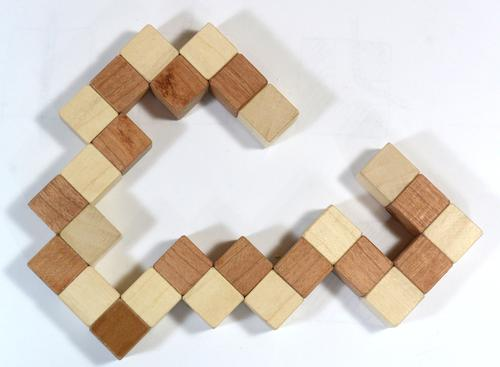
\includegraphics[width=.6\textwidth]{images/snake-cube.jpg}
\end{center}

Oldjuk meg a jól ismert ,,kígyó-kocka'' feladványt!
Az egyes kis szakaszok fixek, de a derékszögű
fordulásoknál egymáson elforgathatóak; a feladat,
hogy kirakjunk belőle egy 3x3-as kockát.

Szokás szerint azzal kezdjük, hogy felvesszük az
adatokat. Ez a készítendő kocka mérete, és a kígyót
alkotó szakaszok hosszai:
\begin{program}
méret(3).
kígyó([3,2,2,3,2,3,2,2,3,3,2,2,2,3,3,3,3]).
\end{program}

A teljes kockán belül minden pozíciót 3
koordinátával tudunk jellemezni:
\begin{program}
pozíció(p(X, Y, Z)) :-
    méret(N), között(1, N, X),
    között(1, N, Y), között(1, N, Z).
\end{program}
Tehát a jelenlegi $3\times3$-as kocka esetében minden
koordináta 1 és 3 között változhat.

A \pr{között} szabály feladatként szerepelt,
így definiálhatjuk:
\begin{program}
között(N, M, N) :- N =< M.
között(N, M, X) :-
    N < M, N1 is N + 1,
    között(N1, M, X).
\end{program}
\index{\pr{között}}
Itt arra érdemes figyelni, hogy \pr{N > M} esetén ez
nem kielégíthető.

Hatféle irányról beszélhetünk, a három tengely
irányában pozitív és negatív irányban. Ezeket
leírhatjuk olyan módon, mint pl. \pr{i(x, -1)} vagy
\pr{i(z, 1)}. Az összes irányt tehát így
fogalmazhatjuk meg:
\begin{program}
irány(i(T,I)) :-
    tartalmaz(T, [x,y,z]),
    tartalmaz(I, [-1,1]).
\end{program}
A \pr{T} itt az egyik tengely, az \pr{I} pedig 1
vagy -1, ami a pozitív ill. negatív irányt jelöli.

Két egymás után következő szakasz mindig merőleges
egymásra, tehát a \emph{tengelyük} nem lehet azonos:
\begin{program}
köv_irány(i(T,_), i(T1,I)) :-
    irány(i(T1,I)), T \= T1.
\end{program}

Hogyan változik egy pozíció, ha ellépünk egy adott
irányban? A \pr{lépés(P1, I, P2)} akkor lesz igaz,
amikor a \pr{P1}-ből \pr{I} irányba ellépve a
\pr{P2}-be jutunk:
\begin{program}
lépés(p(X,Y,Z), i(x,I), p(X1,Y,Z)) :- X1 is X + I.
lépés(p(X,Y,Z), i(y,I), p(X,Y1,Z)) :- Y1 is Y + I.
lépés(p(X,Y,Z), i(z,I), p(X,Y,Z1)) :- Z1 is Z + I.
\end{program}
(Ezért volt jó a pozitív/negatív irányt 1-el és
-1-el jelölni.)

Próbáljuk meg felírni a megoldást! Legyen erre a
szabályunk \pr{megoldás(K, PL, I, X)}; itt \pr{K} a
kígyó hátralevő része, \pr{PL} a már kitöltött
pozíciók listája (az elején a kígyó feje, amit épp
vizsgálunk), az \pr{I} az aktuális irány, és \pr{X}
az irányváltoztatások listája. A reláció akkor
teljesül, ha a \pr{PL} pozíció-lista első elemétől
\pr{I} irányban indulva le tudjuk rakni a \pr{K}
listában levő szakaszokat az \pr{X} listában levő
irányokat követve úgy, hogy mindig a kockán belül
maradunk, és nem megyünk bele a \pr{PL} egyik
elemébe sem. Ekkor a
\begin{query}
?- kígyó(K), pozíció(P), irány(I),
   megoldás(K, [P], I, X).
\end{query}
kérdésre \pr{P} adja a kezdő pozíciót, \pr{I} a
kezdő irányt, és \pr{X} az irányváltoztatásokat.

Ha a kígyónak már csak 1 szakasza van hátra, akkor
csak azt kell megnézni, hogy azt le tudjuk-e tenni:
\begin{program}
megoldás([N], PL, I, [I]) :- ellenőriz(PL, I, N, _).
\end{program}
Az \pr{ellenőriz(PL, I, N, PL1)} akkor lesz igaz, ha
a \pr{PL} elején levő pozícióról az \pr{I} irányban
le tudunk helyezni egy \pr{N} hosszú szakaszt
anélkül, hogy kimennénk a kockából vagy érintenénk
egy \pr{PL}-ben levő pozíciót, és az így bővült
pozíció-lista a \pr{PL1}.

Ezt szavakban elmondani bonyolultabb, mint
programban:
\begin{program}
ellenőriz(PL, _, 1, PL).
ellenőriz([P|M], I, N, PL1) :-
    N > 1, lépés(P, I, P1),
    pozíció(P1), nemtartalmaz(P1, M), N1 is N - 1,
    ellenőriz([P1, P|M], I, N1, PL1).
\end{program}
Ha a szakasz 1 kockából áll, akkor nincs további
teendőnk, és \pr{PL1 = PL}. Egyébként teszünk a
megadott irányban egy lépést, megnézzük, hogy
érvényes pozíció-e, nem szerepel-e az eddigi
pozíciók listájában, és ha ez mind jó, akkor jöhet a
többi lépés -- ehhez a \pr{PL}-et kiegészítjük az új
\pr{P1} pozícióval, és a készítendő szakasz hosszát
csökkentjük 1-el.

Ha a kígyó több szakaszból áll, akkor először
ellépünk az első szakasz hosszával az aktuális
irányban, utána új irányt választunk, és rekurzióval
elvégezzük a maradékot:
\begin{program}
megoldás([N|M], PL, I, [I|X]) :-
    ellenőriz(PL, I, N, PL1), köv_irány(I, I1), 
    megoldás(M, PL1, I1, X).
\end{program}

Ezzel a fent ismertetett módon megkapjuk a
megoldást, de kicsit nehezen olvasható
alakban. Fordítsuk le magyarra az irányokat!
\begin{program}
fordít([], []).
fordít([i(T, I)|M], [F|FM]) :-
    (  T = x, (I = 1, F = jobbra; I = -1, F = balra)
     ; T = y, (I = 1, F = fel;    I = -1, F = le)
     ; T = z, (I = 1, F = előre;  I = -1, F = hátra)
    ), 
    fordít(M, FM).
\end{program}
A \pr{fordít} szabály első argumentuma irányok egy
listája, a második pedig az ennek megfelelő
fordítások listája. Érdemes megfigyelni a
zárójelezés és a logikai vagy jelentésű
pontosvesszők használatát.

Végül akkor tegyük az egész megoldót egy szabályba!
\begin{program}
kígyó_kocka(K, P, FI, FX) :-
    kígyó(K), pozíció(P), irány(I),
    megoldás(K, [P], I, X), fordít([I|X], [FI|FX]).
\end{program}

Ha kipróbáljuk:
\begin{query}
?- kígyó_kocka(K, P, FI, FX).
FI = jobbra,
FX = [jobbra, fel, balra, előre, fel, hátra, jobbra,
      előre, le, balra, fel, hátra, fel, előre, le,
      jobbra, fel],
K = [3, 2, 2, 3, 2, 3, 2, 2, 3, 3, 2, 2, 2, 3, 3, 3,
     3],
P = p(1, 1, 1)
\end{query}
... az eredmény már sokkal könnyebben értelmezhető.

A megoldó elég általános ahhoz, hogy más
változatokra is használható legyen, pl. a ,,mean
green'' feladványra, ha lecseréljük a \pr{kígyó}
definícióját:
\begin{program}
kígyó([3,3,2,3,2,3,2,2,2,3,3,3,2,3,3,3]).
\end{program}
Egy másik variáns a ,,king'' feladvány, amelynél
$4\times4$-es kockát kell építeni:
\begin{program}
méret(4).
kígyó([3,2,3,2,2,4,2,3,2,3,2,3,2,2,2,2,
       2,2,2,2,3,3,2,2,2,2,2,3,4,2,2,2,
       4,2,3,2,2,2,2,2,2,2,2,2,4,2]).
\end{program}
Ennek sokkal több lehetőséget kell megvizsgálnia,
ezért kell neki pár perc.

Megfordíthatjuk a kérdést: hogyan lehet egy
számsorozatot készíteni, ami olyan kígyót határoz
meg, amelyből kocka készíthető? Ehhez a \pr{kígyó}-nak
egy új definíciójára lesz szükségünk:
\begin{program}
kígyó(K) :-
    méret(N), N3 is N^3, N1 is N3 // (N - 1),
    között(N1, N3, H), hossz(K, H),
    kígyó(K, N3).
\end{program}
A teljes kígyó hossza a méret köbe (\pr{N3}). A
kígyót alkotó szakaszok száma (a kígyónak, mint
szakasz-listának a \emph{hossza}, \pr{H}) tehát
\pr{N3/(N-1)} és \pr{N3} között lesz, hiszen minden
szakasz legfeljebb \pr{N-1} új pozíciót fedhet
le. Az egyes szakaszokat ezután a \pr{kígyó/2}
segítségével készítjük el:
\begin{program}
kígyó([], 1).
kígyó([Sz|K], M) :-
    M > 1, méret(N), között(2, N, Sz),
    M1 is M - Sz + 1, kígyó(K, M1).
\end{program}
Ha még \pr{M} hosszú kígyót kell csinálni, akkor
választunk egy számot 2 és \pr{N} között (egy
szakasz hossza csak ilyen lehet), ez lesz a mostani
szakaszunk hossza, és a maradék szakaszokkal pedig
egy ennyivel rövdebb kígyót csinálunk (pontosabban
eggyel hosszabbat, mert egy szakasz utolsó eleme
egyben a következő első eleme). Amikor már csak 1
hosszú kígyót kell csinálni, készen vagyunk.

Ezzel a definícióval azt kapjuk, hogy
\begin{query}
?- kígyó_kocka(K, P, FI, FX).
K = [2, 3, 3, 2, 3, 3, 3, 3, 3, 3, 3, 2, 3, 2, 3],
P = p(1, 2, 2),
FI = le,
FX = [le, jobbra, fel, hátra, le, balra, fel, előre,
      le, jobbra, fel, balra, hátra, le, előre] 
\end{query}
(Ez jó sokáig tart.) Mivel a szakaszok számával
alulról felfele próbálkozunk, az első megoldás a
legkevesebb szakaszból álló kígyó (15 db), amit
$3\times3$-as kockába lehet rendezni. Ha a fenti
definícióban a \pr{között(N1, N3, H)} helyett \pr{H
  = 15}-öt írunk (tehát ha lerögzítjük a szegmensek
számát), akkor gyorsan lefut.

A futási idő mindig egy kompromisszum: (aránylag)
keveset kellett gondolkodnunk ahhoz, hogy megírjuk
ezt a programot. Hatékonyabb programot gyakran
nehezebb írni, viszont néha elég a lassabb is,
pl.~olyan feladatoknál, mint a kígyó-generálás,
amikor a lényeg csak az, hogy találjunk egy
megoldást (még ha akár napokig is kell a gépnek
számolnia). Azért persze törekedjünk a
hatékonyságra!

\subsection*{A teljes program}

Mivel ez már egy elég összetett program volt, itt
van egyben az egész:

\begin{program}
tartalmaz(X, [X|_]).
tartalmaz(X, [_|M]) :- tartalmaz(X, M).

nemtartalmaz(_, []).
nemtartalmaz(X, [Y|M]) :- X \= Y, nemtartalmaz(X, M).

hossz([], 0).
hossz([_|M], N) :- hossz(M, N1), N is 1 + N1.

között(N, M, N) :- N =< M.
között(N, M, X) :-
    N < M, N1 is N + 1,
    között(N1, M, X).

% Standard
méret(3).
kígyó([3,2,2,3,2,3,2,2,3,3,2,2,2,3,3,3,3]).

% Mean green
% méret(3).
% kígyó([3,3,2,3,2,3,2,2,2,3,3,3,2,3,3,3]).

% King
% méret(4).
% kígyó([3,2,3,2,2,4,2,3,2,3,2,3,2,2,2,2,
%        2,2,2,2,3,3,2,2,2,2,2,3,4,2,2,2,
%        4,2,3,2,2,2,2,2,2,2,2,2,4,2]).

% Generáló
% méret(3).
% kígyó(K) :-
%     méret(N), N3 is N^3, N1 is N3 // (N - 1),
%     között(N1, N3, H), hossz(K, H),
%     kígyó(K, N3).
% kígyó([], 1).
% kígyó([Sz|K], M) :-
%     M > 1, méret(N), között(2, N, Sz),
%     M1 is M - Sz + 1, kígyó(K, M1).

pozíció(p(X, Y, Z)) :-
    méret(N), között(1, N, X),
    között(1, N, Y), között(1, N, Z).

irány(i(T,I)) :-
    tartalmaz(T, [x,y,z]),
    tartalmaz(I, [-1,1]).

köv_irány(i(T,_), i(T1,I)) :-
    irány(i(T1,I)), T \= T1.

lépés(p(X,Y,Z), i(x,I), p(X1,Y,Z)) :- X1 is X + I.
lépés(p(X,Y,Z), i(y,I), p(X,Y1,Z)) :- Y1 is Y + I.
lépés(p(X,Y,Z), i(z,I), p(X,Y,Z1)) :- Z1 is Z + I.

ellenőriz(PL, _, 1, PL).
ellenőriz([P|M], I, N, PL1) :-
    N > 1, lépés(P, I, P1),
    pozíció(P1), nemtartalmaz(P1, M), N1 is N - 1,
    ellenőriz([P1, P|M], I, N1, PL1).

megoldás([N], PL, I, [I]) :- ellenőriz(PL, I, N, _).
megoldás([N|M], PL, I, [I|X]) :-
    ellenőriz(PL, I, N, PL1), köv_irány(I, I1), 
    megoldás(M, PL1, I1, X).

fordít([], []).
fordít([i(T, I)|M], [F|FM]) :-
    (  T = x, (I = 1, F = jobbra; I = -1, F = balra)
     ; T = y, (I = 1, F = fel;    I = -1, F = le)
     ; T = z, (I = 1, F = előre;  I = -1, F = hátra)
    ), 
    fordít(M, FM).

kígyó_kocka(K, P, FI, FX) :-
    kígyó(K), pozíció(P), irány(I),
    megoldás(K, [P], I, X), fordít([I|X], [FI|FX]).
\end{program}

% -*- fill-column: 52 -*-
% (local-set-key (kbd "C-c C-f") 'display-fill-column-indicator-mode)
\chapter{Vezérlés}
\section{Rendezések}
Egy klasszikus -- és nagyon hasznos -- programozási
feladat számok listájának növekvő sorrendbe
rendezése. Erre rengeteg módszer van, itt csak a
legfontosabbak közül nézünk meg néhányat.

\subsection*{Beszúrásos rendezés}
Az első algoritmus a \emph{beszúrásos rendezés}. Az
ötlet a következő: ha van egy listám, akkor azt
szétszedem az első elemre és a maradékára, az
utóbbit (rekurzívan) rendezem, és végül az első
elemet beszúrom a ,,megfelelő'' helyre.
\index{rendezés!beszúrásos}
\begin{program}
rendez1([], []).
rendez1([X|M], Y) :-
    rendez1(M, M1), beszúr(X, M1, Y).
\end{program}
A megfelelő helyre való beszúrásnál pedig egyszerűen
addig megyünk, amíg egy legalább akkora elemet nem
találunk:
\begin{program}
beszúr(X, [], [X]).
beszúr(X, [Y|M], [X,Y|M]) :- X =< Y.
beszúr(X, [Y|M], [Y|M1]) :- X > Y, beszúr(X, M, M1).
\end{program}
Próbáljuk ki!
\begin{query}
?- rendez1([4,1,9,2,6,0,3,2,5,1], X).
X = [0, 1, 1, 2, 2, 3, 4, 5, 6, 9]
\end{query}

Ennek az algoritmusnak egy nagy előnye, hogy akkor
is jól használható, ha az adatokat folyamatosan
kapjuk, hiszen ha már van egy rendezett listánk,
akkor utána mindig elég a \pr{beszúr} műveletet
használni. Egy másik jó tulajdonsága, hogy egy már
rendezett sorozatnál nem végez plusz munkát, épp
csak ellenőrzi, hogy a lista tényleg jó sorrendben
van:
\begin{query}
?- trace, rendez1([1,2,3], X).
Call:rendez1([1, 2, 3], X)
  Call:rendez1([2, 3], X1)
    Call:rendez1([3], X2)
      Call:rendez1([], X3)
      Exit:rendez1([], [])
      Call:beszúr(3, [], X2)
      Exit:beszúr(3, [], [3])
    Exit:rendez1([3], [3])
    Call:beszúr(2, [3], X1)
      Call:2=<3
      Exit:2=<3
    Exit:beszúr(2, [3], [2, 3])
  Exit:rendez1([2, 3], [2, 3])
  Call:beszúr(1, [2, 3], X)
    Call:1=<2
    Exit:1=<2
  Exit:beszúr(1, [2, 3], [1, 2, 3])
Exit:rendez1([1, 2, 3], [1, 2, 3])
X = [1, 2, 3]
\end{query}

Ugyanakkor ha nincs szerencsénk, nem túl jó
hatásfokú: ha a lista $n$ hosszú, akkor kb.~$n^2$
összehasonlítást végez a legrosszabb esetben.

\subsection*{Gyorsrendezés}
A gyorsrendezésnél kiválasztunk egy tetszőleges
elemet (pl.~az elsőt), és a többit két részre
osztjuk aszerint, hogy nagyobb-e ennél vagy
sem. Ezután a két részt külön--külön rendezzük
(rekurzívan), majd az eredmény ezek összefűzéséből
adódik:
\index{rendezés!gyors}
\begin{program}
rendez2([], []).
rendez2([X|M], Y) :-
    szétoszt(X, M, Kicsi, Nagy),
    rendez2(Kicsi, K),
    rendez2(Nagy, N),
    hozzáfűz(K, [X|N], Y).
\end{program}
A szétosztás elég magától értetődő:
\begin{program}
szétoszt(_, [], [], []).
szétoszt(X, [Y|M], K, [Y|N]) :-
    X =< Y, szétoszt(X, M, K, N).
szétoszt(X, [Y|M], [Y|K], N) :-
    X > Y, szétoszt(X, M, K, N).
\end{program}

Ez (nagyon hosszú listákra) bizonyíthatóan sokkal
kevesebb ellenőrzést végez, mint a beszúrásos
rendezés. A fenti program azonban a hozzáfűzések
miatt nem igazán hatékony -- a következő leckében
majd szó lesz a különbség-listákról, amelyek
segítségével sokkal gyorsabbá tehető.

\subsection*{Fésülő rendezés}
Utolsónak nézzünk meg egy nagyon hasonló
algoritmust: itt is két részre bontjuk mindig a
listát, azokat rendezzük, majd összefűzzük, de itt
nem a szétválasztás a bonyolultabb, hanem az
összefűzés, vagy ez esetben az \emph{összefésülés}.
\index{rendezés!fésülő}

A listát a felénél kettéosztjuk, és mindkét részt
rendezzük (rekurzívan), végül a két rendezett listát
egy listává fésüljük össze:
\begin{program}
rendez3([], []).
rendez3([X], [X]).
rendez3(X, Y) :-
    kettéoszt(X, X1, X2),
    rendez3(X1, Y1),
    rendez3(X2, Y2),
    összefésül(Y1, Y2, Y).

kettéoszt([], [], []).
kettéoszt([X], [X], []).
kettéoszt([X,Y|M], [X|M1], [Y|M2]) :-
    kettéoszt(M, M1, M2).
\end{program}

Az összefésülésnél a két lista elemét
összehasonlítjuk, és a megfelelőt berakjuk a
maradékok összefűzéséből kapott listába:
\begin{program}
összefésül([X|Mx], [Y|My], [X|M]) :-
    X =< Y, összefésül(Mx, [Y|My], M).
összefésül([X|Mx], [Y|My], [Y|M]) :-
    X > Y, összefésül([X|Mx], My, M).
összefésül(X, [], X).
összefésül([], Y, Y).
\end{program}

Itt érdekes módon azt tapasztaljuk, hogy a (helyes)
eredményt végtelen sokszor megkapjuk. Ez azért van,
mert a \pr{rendez3} harmadik szabálya az egyelemű
listákra is meghívódhat. Ezt ki lehetne védeni
azzal, hogy megköveteljük, hogy legyen legalább két
eleme:
\begin{program}
rendez3(X, Y) :-
    X = [_,_|_], Y = [_,_|_],
    kettéoszt(X, X1, X2),
    rendez3(X1, Y1),
    rendez3(X2, Y2),
    összefésül(Y1, Y2, Y).
\end{program}
\dots de ez nem a legelegánsabb. (Hasonlóan, az
\pr{összefésül} utolsó két szabálya közt is van
átfedés.) Nincs valami jobb mód erre?

\begin{infobox*}{}{furcsa rendezések}
Rendezési algoritmusokból nincs hiány. Bizonyítható,
hogy a gyorsrendezés, a fésülő rendezés (és még sok
másik) a lehető leghatékonyabb\dots kivéve egy-két
furcsa módszert:
\begin{enumerate}
\item Vágjunk (száraz) spagettitésztákat az egyes
  számoknak megfelelő hosszokra, majd marokra fogva
  tegyük le az asztalra. Ezután egy kartonlapot
  rátéve mindig sorban vegyük ki azt, ami hozzáér a
  laphoz, és így egy csökkenő sorrendezéshez jutunk.
\item Vegyük a lista egy véletlenszerű
  permutációját, és ellenőrizzük, hogy sorban
  van-e. Ha igen, készen vagyunk. Ha nem, akkor
  robbantsuk fel a világot. Feltéve, hogy igaz a
  párhuzamos univerzumok elmélete, csak az az
  univerzum fog megmaradni, amelyikben a véletlen
  permutáció pont a helyes sorbarendezés volt.
\end{enumerate}
\index{rendezés!spagetti}\index{rendezés!véletlen}
\end{infobox*}      

\section{Vágás}
Egy szabály törzsében \emph{vágást} eszközölhetünk a
\pr{!} segítségével. Ez azt mondja, hogy ha már
idáig eljutottunk, akkor vagy sikerül teljesíteni a
törzs maradék részét, vagy ha nem, akkor úgy
vesszük, hogy ezzel a fejjel való egyesítés
sikertelen volt, nem próbálunk a \pr{!} előtti
kifejezésekre visszamenni, vagy az azonos fejhez
tartozó esetleges többi szabályt megnézni.
\index{vagas@vágás}\index{\pr{"!}}

Nézzük meg például az alábbi szabályokat, ahol
\pr{A}, \pr{B}, \pr{C} stb. kifejezéseket jelölnek:
\begin{program}
C :- P, Q, R, !, S, T, U.
C :- V.

A :- B, C, D.
\end{program}

Ekkor ha az
\begin{query}
?- A.
\end{query}
kérdést feltesszük, a következő fog történni:
\begin{enumerate}
\item Megnézi, hogy \pr{B} teljesül-e (tegyük fel,
  hogy igen).
\item Megnézi, hogy \pr{P}, \pr{Q}, \pr{R}
  teljesülnek-e (tegyük fel, hogy igen).
\item Megnézi, hogy \pr{S}, \pr{T}, \pr{U}
  teljesülnek-e. Tegyük fel, hogy az \pr{S} és
  \pr{T} teljesül, de az \pr{U} nem. Ekkor szokás
  szerint visszamegy a \pr{T}-re, és megkeresi annak
  egy másik megoldását stb.
\item Ha nem sikerült az \pr{S}, \pr{T}, \pr{U}-t
  teljesíteni, akkor -- a vágás miatt -- már nem
  megy vissza, hogy az \pr{R} egy másik megoldását
  keresse, és nem próbálkozik a \pr{C}-hez tartozó
  második szabállyal sem, hanem egy szinttel feljebb
  megy, és a \pr{B}-hez keres egy másik megoldást.
\end{enumerate}

\subsection*{Összefésülés hatékonyabban}
Nézzük meg, hogyan lehet ezzel feljavítani az összefésülést!
\begin{program}
összefésül([X|Mx], [Y|My], [X|M]) :-
    X =< Y, !, összefésül(Mx, [Y|My], M).
összefésül([X|Mx], [Y|My], [Y|M]) :-
    X > Y, !, összefésül([X|Mx], My, M).
összefésül(X, [], X) :- !.
összefésül([], Y, Y) :- !.
\end{program}

A vágások a programot hatékonyabbá teszik: ha az
első szabályban láttuk, hogy \pr{X =< Y}, már nem
kell ellenőrizni a többi szabályt stb. (Az utolsó
sorban a vágás felesleges, csak a szimmetria
kedvéért került bele.)

Hasonlóan, a \pr{rendez3} második szabályában:
\begin{program}
rendez3([X], [X]) :- !.
\end{program}
Ezekkel a módosításokkal már egyértelmű
(\emph{determinisztikus}) lesz a megoldás.
\index{determinisztikusság}

A vágások nem változtatják meg a program értelmét
(tehát, hogy milyen kifejezésekre lesz igaz), csak a
hatékonyságát.

\subsection*{Maximum}
Nézzünk egy másik példát! Az alábbi szabály két szám
közül kiválasztja a nagyobbikat:
\begin{program}
max1(X, Y, X) :- X >= Y.
max1(X, Y, Y) :- X < Y.
\end{program}
A fenti módon ez átírható így:
\begin{program}
max2(X, Y, X) :- X >= Y, !.
max2(X, Y, Y) :- X < Y.
\end{program}

Felmerül azonban ekkor, hogy a második szabályban szükség
van-e egyáltalán az \pr{X < Y} összehasonlításra,
hiszen csak akkor juthatunk oda, ha az \pr{X >= Y}
nem teljesült. A program akkor is működni látszik,
ha elhagyjuk:
\begin{program}
max3(X, Y, X) :- X >= Y, !.
max3(_, Y, Y).
\end{program}

Teszteljük egy kicsit!
\begin{query}
?- max3(3, 5, X).
X = 5
?- max3(4, 2, X).
X = 4
?- max3(1, 5, 5).
true
?- max3(5, 1, 1). % Ajjaj...
true
\end{query}

Hoppá! Mi történt?  Mivel az utolsó példában
mindhárom argumentumnak van értéke, és az első és
harmadik nem azonos, az első szabállyal nem is
próbálkozik, hanem rögtön a másodikra megy, ami
pedig most, hogy kivettük a feltételt, teljesül.

A \pr{max3} változatban megváltozott a program
deklaratív jelentése, hiszen egy olyan tényt
tartalmaz, ami magában nézve nem igaz. Ez általában
kerülendő, bár a hatékonysághoz néha szükséges. Ha
ilyen gondolatmenetet alkalmazunk, nagyon óvatosnak
kell lenni -- itt pl. biztosnak kell lennünk benne,
hogy a harmadik argumentum mindig változó.

\subsection*{Hozzáadás halmazhoz}
Egy további példaként nézzük meg az alábbi szabályt:

\begin{program}
% hozzáad(+X, +Halmaz, -Eredmény).
% Hozzáadja X-et a Halmaz listához,
% de csak akkor, ha az még nem tartalmazta.
hozzáad(X, L, L) :- tartalmaz(X, L), !.
hozzáad(X, L, [X|L]).
\end{program}

A vágás nélkül itt a második szabályt nehezebb lenne
megfogalmazni, kéne hozzá a 3. leckéhez tartozó
projektben látott \pr{nemtartalmaz} szabály, és
következésképp a hatékonyságból is vesztene.

Cserébe itt is problémába ütközünk, ha a harmadik
argumentum nem változó:
\begin{query}
?- hozzáad(b, [a,b], [b,a,b]).
true
\end{query}
Ezt elkerülendő, érdemes a dokumentációval\index{dokumentáció}
egyértelművé tenni a használatot. A fenti programhoz
tartozó megjegyzés is ilyen szellemben íródott. Az
első sorában egy egyezményes jelölésrendszert
használ, melyben minden argumentum háromféle lehet:
\begin{itemize}
\item \pr{+X} : kell, hogy legyen értéke
\item \pr{?X} : lehet értéke, de nem muszáj
\item \pr{-X} : csak változó lehet
\end{itemize}
Például:
\begin{enumerate}
\item \pr{+X > +Y} [4.~lecke]
\item \pr{lapít(+Eredeti, -Lapos)} [3.~lecke]
\item \pr{tartalmaz(?Elem, ?Lista)} [3.~lecke]
\end{enumerate}
Az első esetben mindkét kifejezésnek ismertnek kell
lennie; a másodikban a lapítandó lista ismert, és a
lapított verzió csak változó lehet; a harmadikban
pedig mind a lista, mind a benne tartalmazandó elem
lehet változó vagy ismert is.

\begin{problem}
Nézzük meg az alábbi szabályokat!
\begin{program}
p(1).
p(2) :- !.
p(3).
\end{program}       
Mit lesz az összes válasz az alábbi kérdésekre:
\begin{query}
?- p(X).
?- p(X), p(Y).
?- p(X), !, p(Y).
\end{query}
\end{problem}
\begin{problem}
Írd át hatékonyabbra a \pr{szétoszt} szabályt
vágások segítségével!
\end{problem}

\section{Tagadás}
Hogyan tudjuk megfogalmazni azt, hogy ,,Csilla
szeret minden állatot, kivéve a pókokat''?
\begin{program}
szereti(csilla, X) :- pók(X), !, fail.
szereti(csilla, X) :- állat(X).
\end{program}
(Általában ilyenkor a \pr{false} helyett a
\pr{fail}-t szokás használni, de a kettő jelentése
azonos.)\index{\pr{fail}}\index{tagadás}

Próbáljuk ki!
\begin{program}
állat(tarantula).
állat(denevér).
pók(tarantula).
\end{program}
\begin{query}
?- szereti(csilla, tarantula).
false
?- szereti(csilla, denevér).
true
\end{query}
Ez annyira hasznos, hogy érdemes bevezetni, mint
tagadást:
\begin{program}
nem(P) :- P, !, fail.
nem(_).
\end{program}

Figyeljük meg, hogy itt valami olyat csináltunk,
amit eddig még soha: egy változót (\pr{P}) a
törzsben magában használtunk. Ez feltételezi, hogy a
\pr{P}-nek kiszámolható az igazságértéke. Például a
fenti példát átírva:
\begin{program}
szereti(csilla, X) :- állat(X), nem(pók(X)).
\end{program}
Itt a \pr{P} értéke a \pr{pók(X)} struktúra, és a
\pr{nem} törzsében levő \pr{P} kiértékelésekor ezt
mint megoldandó célkifejezést értelmezi.

\subsection*{A ,,zárt világ'' feltétel}
A tagadásnak ez a módja nem mindig intuitív. Egy így
tagadott kifejezés akkor lesz igaz, ha a kifejezés
nem bizonyítható.\index{zart@zárt világ}

Mi történik, ha az előző programban felcseréljük a
törzs két tagját?
\begin{program}
szereti(csilla, X) :- nem(pók(X)), állat(X).
\end{program}
Érdekes módon Csilla most már a denevéreket sem
szereti! Miért? Azért, mert a \pr{nem(pók(X))}-ben
az \pr{X} egy változó, tehát a \pr{pók(X)}
bizonyítható az \pr{X = tarantula} helyettesítéssel,
így a \pr{nem(pók(X))} nem teljesül. Az érték
nélküli argumentumokkal tehát vigyázni kell.

Hasonlóan furcsa lehet, hogy
\begin{query}
?- nem(állat(kutya)).
true
\end{query}
\dots de persze helyes, hiszen a programban levő
szabályok alapján nem bizonyítható, hogy a kutya
állat.

Ezek miatt a \pr{nem} (vagy az angol \pr{not})
helyett a \pr{\textbackslash+} operátort szokás
használni, melynek definíciója ugyanaz, csak az
elnevezés kevésbé félrevezető:
\begin{program}
szereti(csilla, X) :- állat(X), \+ pók(X).
\end{program}
\index{\pr{\textbackslash+}}

\begin{problem}
Milyen kérdéssel lehet a \pr{Jelöltek} listából
kiválasztani azokat, akik nem szerepelnek a
\pr{Kiesettek} listában? Használjátok a
\pr{tartalmaz} szabályt és a tagadást!
\end{problem}
\begin{problem}
Készítsetek szabályt, ami két halmaz különbségét
képzi! (A halmaz itt egy olyan lista, amiben minden
elem egyszer fordul elő.)
\begin{query}
?- különbség([a,b,c,d], [f,d,b,e], X).
X = [a, c]
\end{query}
\end{problem}
\begin{problem}
Készítsetek szabályt, ami kiválogatja egy listából
azokat a kifejezéseket, amelyek egy adott másik
kifejezéssel egyesíthetőek!
\begin{query}
?- egyesíthető([X,b,t(Y)], t(a), L).
L = [X, t(Y)]
\end{query}
Figyeljetek arra, hogy az \pr{X} és \pr{Y} ne kapjon
ezáltal értéket!
\end{problem}

\section{Projekt: Katamino}
Készítsünk megoldót a Katamino-feladványokhoz!

\begin{center}
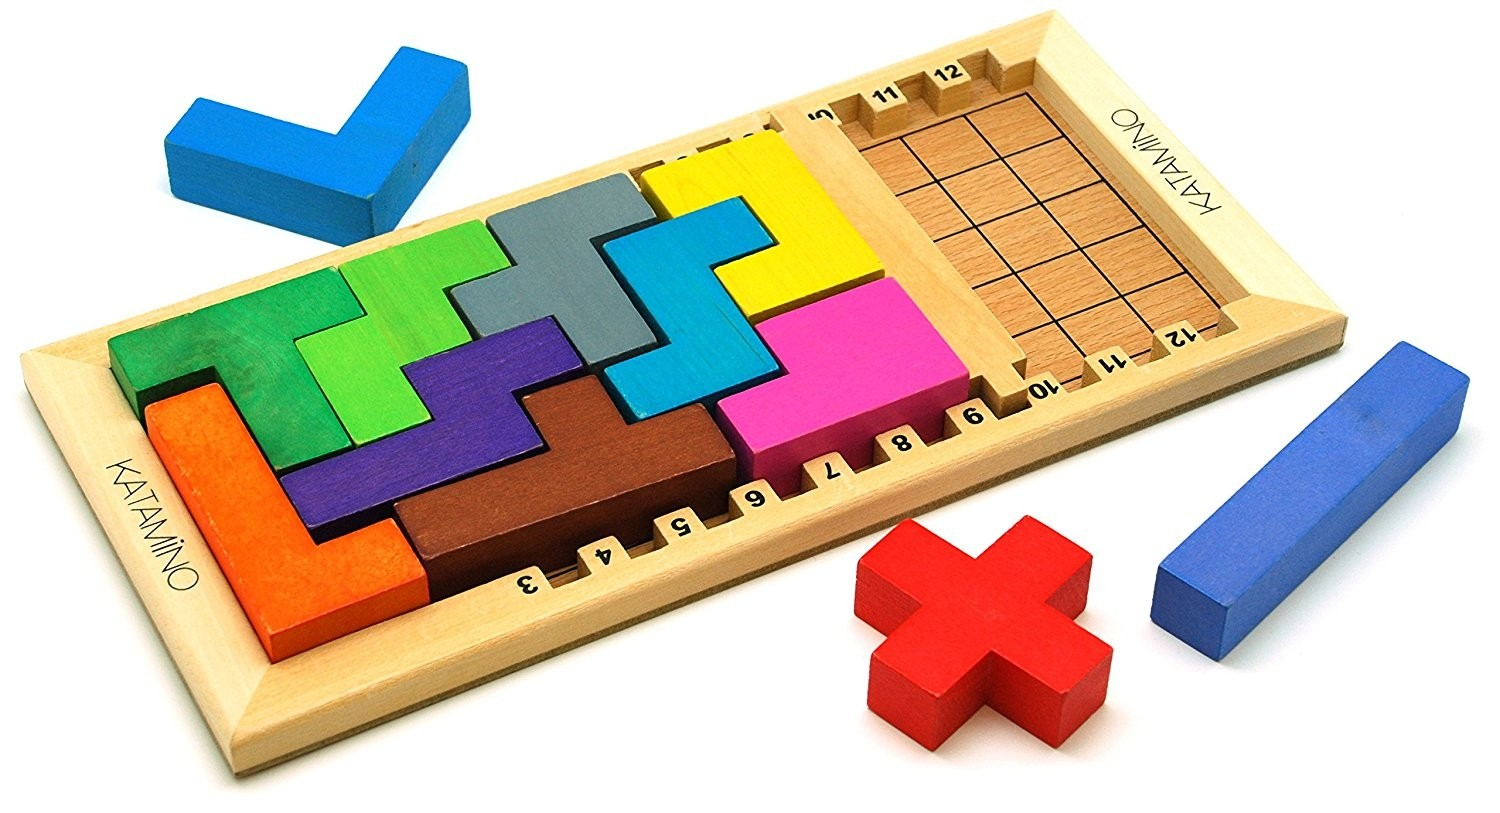
\includegraphics[width=\textwidth]{images/katamino.jpg}
\end{center}

A feladat mindig az, hogy a 12 pentominó egy adott
részhalmazából rakjunk ki egy $5\times n$-es
téglalapot.

\subsection*{Reprezentáció}
Az első lépés továbbra is az, hogy valahogyan le
kell írni a gép számára az adatokat, vagyis a
használható alakzatokat. Sokféle leírás
elképzelhető; itt most csináljuk a következőt:
minden egyes alakzatot a körülírható téglalap bal
alsó sarkához képest számolt koordinátáival írjuk
le.

Például a T-alakzatnál:
\begin{center}
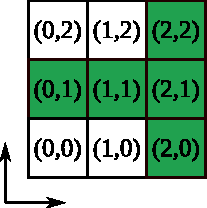
\includegraphics[width=.3\textwidth]{images/pentomino.pdf}
\end{center}
Ha a bal alsó sarok a $(0,0)$ pont, akkor az
alakzathoz tartozó pontok a következők: $(0,1)$,
$(1,1)$, $(2,0)$, $(2,1)$ és $(2,2)$. A pontokat
$x$-koordináta szerint, és azon belül $y$-koordináta
szerint rendezve írjuk fel.

Az $x$ és $y$-koordináták összefogására bármilyen
struktúrát használhatunk, pl. \pr{p(0,1)}, de a
tömörség kedvéért szokás a \pr{-} operátort
alkalmazni: \pr{0-1}. Bár az egyes
forgatások/tükrözések programból is legenerálhatóak,
egyszerűbb mindegyiket külön adatként megadni.

A T esetében pl.:
\begin{program}
alakzat(t, [0-0,0-1,0-2,1-1,2-1]).
alakzat(t, [0-0,1-0,1-1,1-2,2-0]).
alakzat(t, [0-1,1-1,2-0,2-1,2-2]).
alakzat(t, [0-2,1-0,1-1,1-2,2-2]).
\end{program}

Hasonlóan lehet definiálni a többi alakzatot,
amelyek mind valamilyen 1 betűből álló kódot kaptak:
\pr{k}, \pr{p}, \pr{c} stb. (Az összes alakzat, a
teljes program forráskódjával együtt, a lecke végén
található.)

\subsection*{Megoldó}
A programunk fő szabálya a \pr{kirak} lesz, ami egy
alakzat-listához megadja, hogy hogyan fog kinézni a
tábla. A megoldás módszere nagyon egyszerű: mindig a
(balról/alulról) első lyukat próbáljuk betömni.

\begin{program}
kirak(Ak, X) :- hossz(Ak, N), kirak(Ak, N, [], X).

kirak([], _, T, T).
kirak(Ak, N, T, X) :-
    első_lyuk(N, T, P),
    töröl(A, Ak, Ak1),
    letesz(A, P, N, T, T1),
    kirak(Ak1, N, T1, X).
\end{program}
A 2-argumentumú változat megnézi, hogy hány
alakzatot kapott (tehát milyen hosszú a tábla), és
meghívja a 4-argumentumú testvérét. Ez a
felhasználható alakzatokon (\pr{Ak}) kívül még
megkapja a tábla hosszát (\pr{N}), a tábla jelenlegi
állapotát (\pr{T}), és ezáltal kiszámolja a
kitöltött táblát (\pr{X}).

Ehhez megkeresi az első lyukat, majd kiválaszt
(töröl) egy alakzatot, azt leteszi úgy, hogy lefedje
a lyukat, és rekurzívan folytatja a műveletet, amíg
mindent le nem rak.

A tábla állapotát egy listában tároljuk, aminek az
elemei \pr{h(X-Y,A)} alakban adják meg, hogy az
\pr{X-Y} pozíción az \pr{A} alakzat egy darabja
található. Az első lyuk megkeresése így nagyon
egyszerű:
\begin{program}
első_lyuk(N, T, X-Y) :-
    között(1, N, X), között(1, 5, Y),
    \+ tartalmaz(h(X-Y,_), T), !.
\end{program}

Visszatérve az \pr{első\_lyuk}-ra, ez deklaratív
olvasatban azt mondja, hogy az \pr{X-Y} koordináták
a megfelelő keretek között vannak, és a tábla ezen a
pozíción nem tartalmaz elemet. Mitől fogja ez az
elsőt adni? Azért, mert a procedurális olvasatból
tudjuk, hogy sorban fog próbálkozni, tehát először
az \pr{X = 1} eseteket próbálja végig különböző
\pr{Y} értékekre, aztán az \pr{X = 2}-t stb., és a
végén levő vágásnak köszönhetően nem fog további
lyukakat megadni akkor sem, ha a keresés visszalépne
ide.

Már csak a \pr{letesz(A, X-Y, N, T, T1)} szabály van
hátra. Ez megpróbálja az \pr{A} alakzatot lerakni
úgy, hogy lefedje az \pr{X-Y} pontot, ne menjen ki
az $5\times n$-es táblából, és ne takarjon olyan
pozíciókat, amelyek szerepelnek \pr{T}-ben. Ha
sikerül, akkor az alakzat lehelyezésével kapott új
tábla a \pr{T1}.
\begin{program}
letesz(A, X-Y, N, T, T1) :-
    alakzat(A, [_-Dy|Dk]),
    Y1 is Y - Dy, Y1 > 0,
    letesz(A, X-Y1, Dk, N, [h(X-Y,A)|T], T1).
\end{program}
Ez tehát az \pr{A} alakzatnak kiválasztja egy
forgatását, és megnézi az első pontjának az
$y$-koordinátáját (\pr{Dy}). Az \pr{Y} koordinátánál
ennyivel lejjebb kell rakni az alakzatot, hogy az
első pont fedje a lyukat (hiszen az első pont az
alakzat legbaloldalibb, és azon belül legalsó
pontja). Ha ez a módosult \pr{Y1} koordináta nem
pozitív, akkor az alakzat kilóg.

A tényleges lerakási kísérletet a \pr{letesz}
6-argumentumú változata végzi:
\begin{program}
letesz(_, _, [], _, T, T).
letesz(A, X-Y, [Dx-Dy|Dk], N, T, T1) :-
    X1 is X + Dx, között(1, N, X1),
    Y1 is Y + Dy, között(1, 5, Y1),
    \+ tartalmaz(h(X1-Y1,_), T),
    letesz(A, X-Y, Dk, N, [h(X1-Y1,A)|T], T1).
\end{program}
Ez plusz argumentumként megkapja a kiválasztott
forgatáshoz tartozó pontokat is (az első kivételéve,
amivel a lyukat fedtük), és ezeken megy végig
rekurzívan. Minden lépésben a (módosított) \pr{X-Y}
koordináta alapján kiszámolja, hogy hova kerül a
pont, és ellenőrzi, hogy értelmes-e a koordináta és
nincs-e már lefedve \pr{T}-ben.

\subsection*{Kiíratás}
A lényeggel ugyan már készen vagyunk, de az eredmény
nehezen olvasható:
\begin{query}
?- kirak([l,t,w,k,y,r,z,c,p], X).
  X = [h(9-5, c), h(9-4, c), h(9-3, c), h(8-5, c),
       h(8-3, c), h(9-2, p), h(9-1, p), h(8-2, p),
       h(8-1, p), h(7-1, p), h(8-4, z), h(7-4, z),
       h(7-3, z), h(7-2, z), h(6-2, z), h(7-5, r),
       h(6-5, r), h(6-4, r), h(6-3, r), h(5-4, r),
       h(5-5, w), h(4-5, w), h(4-4, w), h(3-4, w),
       h(3-3, w), h(6-1, y), h(5-2, y), h(5-1, y),
       h(4-1, y), h(3-1, y), h(5-3, k), h(4-3, k),
       h(4-2, k), h(3-2, k), h(2-2, k), h(3-5, t),
       h(2-5, t), h(2-4, t), h(2-3, t), h(1-5, t), 
       h(2-1, l), h(1-4, l), h(1-3, l), h(1-2, l),
       h(1-1, l)]
\end{query}

Próbáljuk meg kiíratni egy kicsit ,,grafikusabb''
formában! Az elsődleges szabályunk akkor ez lesz:
\begin{program}
katamino(Ak) :-
    hossz(Ak, N), kirak(Ak, X), kiír(N, X).
\end{program}

A \pr{kiír(N, T)} pedig 5 sorba rendezve szépen
kiírja az \pr{N} hosszú \pr{T} táblát. A kiíráshoz a
\pr{write(X)} kifejezést fogjuk használni, ami
kiírja az \pr{X} értékét, új sor nyitásához pedig a
\pr{nl}-t (\emph{newline}, újsor).
\index{\pr{write}}\index{\pr{nl}}
\begin{program}
kiír(N, T) :- kiír(N, 1-5, T).

kiír(_, _-0, _).
kiír(N, X-Y, T) :-
    Y =< 5, X > N, Y1 is Y - 1,
    nl, kiír(N, 1-Y1, T).
kiír(N, X-Y, T) :-
    Y =< 5, X =< N,
    tartalmaz(h(X-Y,A), T),
    write(A), write(' '),
    X1 is X + 1,
    kiír(N, X1-Y, T).
\end{program}
A 2-argumentumú változat csak átadja a feladatot a
3-argumentumúnak, ami megkapja az éppen kiírandó
elem \pr{X-Y} koordinátáját is. Ennek három szabálya
van:
\begin{enumerate}
\item Ha már a 0. sort kéne kiírni, készen vagyunk.
\item Ha \pr{X > N}, akkor vége az aktuális sornak,
  új sort kezdünk. Az \pr{Y} koordináta felülről
  megy lefelé, mert a kiírás is felülről lefelé
  történik.
\item Egyébként megkeresi, hogy az \pr{X-Y} pozíción
  melyik alakzat található, és kiírja, utána kiír
  még egy szóközt, és továbbmegy a következő \pr{X}
  pozícióra.
\end{enumerate}
Nézzük meg!
\begin{query}
?- katamino([l,t,w,k,y,r,z,c,p]).
t t t w w r r c c 
l t w w r r z z c 
l t w k k r z c c 
l k k k y z z p p 
l l y y y y p p p 
true
\end{query}
És ez éppen az a megoldás, ami a képen van! Erre
persze elég jó esély volt, ugyanis a felhasználandó
alakzatok listáját hozzávetőlegesen a képen látható
megoldás sorrendjében adtuk meg. Egy másik
permutáció más megoldást talál meg először:
\begin{query}
?- katamino([t,w,l,k,r,z,y,p,c]).
w y y y y l l l l 
w w y p p p r r l 
t w w p p z z r r 
t t t k k z c r c 
t k k k z z c c c 
true 
\end{query}

\begin{problem}
A Katamino szabályai szerint a kirakandó téglalap
magassága mindig 5. Oldjuk fel ezt a korlátot!
Írjátok át a programot úgy, hogy a \pr{katamino}
szabály paraméterben kapja meg a magasságot is, és
ennek megfelelő megoldást keressen! A program vegye
észre rögtön, ha a magasság nem illik a megkapott
alakzatok számához (pl.~10 alakzat és 7-es
magasság). Keressetek megoldást a $3\times20$,
$4\times15$, $5\times12$, $6\times10$ téglalapok
kitöltésére! (Tipp: a szabályokban az eddigi \pr{N}
paramétert cseréljétek \pr{N-M} párra.)
\end{problem}

\subsection*{A teljes program}
\begin{program}
katamino(Ak) :-
    hossz(Ak, N), kirak(Ak, X), kiír(N, X).

% Megoldó

kirak(Ak, X) :- hossz(Ak, N), kirak(Ak, N, [], X).

kirak([], _, T, T).
kirak(Ak, N, T, X) :-
    első_lyuk(N, T, P),
    töröl(A, Ak, Ak1),
    letesz(A, P, N, T, T1),
    kirak(Ak1, N, T1, X).

első_lyuk(N, T, X-Y) :-
    között(1, N, X), között(1, 5, Y),
    \+ tartalmaz(h(X-Y,_), T), !.

letesz(A, X-Y, N, T, T1) :-
    alakzat(A, [_-Dy|Dk]),
    Y1 is Y - Dy, Y1 > 0,
    letesz(A, X-Y1, Dk, N, [h(X-Y,A)|T], T1).

letesz(_, _, [], _, T, T).
letesz(A, X-Y, [Dx-Dy|Dk], N, T, T1) :-
    X1 is X + Dx, között(1, N, X1),
    Y1 is Y + Dy, között(1, 5, Y1),
    \+ tartalmaz(h(X1-Y1,_), T),
    letesz(A, X-Y, Dk, N, [h(X1-Y1,A)|T], T1).

% Kiírás

kiír(N, T) :- kiír(N, 1-5, T).

kiír(_, _-0, _).
kiír(N, X-Y, T) :-
    Y =< 5, X > N, Y1 is Y - 1,
    nl, kiír(N, 1-Y1, T).
kiír(N, X-Y, T) :-
    Y =< 5, X =< N,
    tartalmaz(h(X-Y,A), T),
    write(A), write(' '),
    X1 is X + 1,
    kiír(N, X1-Y, T).

% Segéd-szabályok

tartalmaz(X, [X|_]).
tartalmaz(X, [_|Maradék]) :- tartalmaz(X, Maradék).

töröl(X, [X|M], M).
töröl(X, [Y|M], [Y|M1]) :- töröl(X, M, M1).

hossz([], 0).
hossz([_|M], N) :- hossz(M, N1), N is 1 + N1.

között(N, M, N) :- N =< M.
között(N, M, X) :-
    N < M, N1 is N + 1,
    között(N1, M, X).

% Alakzatok

% kígyó (lila)
alakzat(k, [0-0,0-1,0-2,1-2,1-3]).
alakzat(k, [0-0,0-1,1-1,1-2,1-3]).
alakzat(k, [0-0,1-0,1-1,2-1,3-1]).
alakzat(k, [0-0,1-0,2-0,2-1,3-1]).
alakzat(k, [0-1,0-2,0-3,1-0,1-1]).
alakzat(k, [0-1,1-0,1-1,2-0,3-0]).
alakzat(k, [0-1,1-1,2-0,2-1,3-0]).
alakzat(k, [0-2,0-3,1-0,1-1,1-2]).
% P-betű (rózsaszín)
alakzat(p, [0-0,0-1,0-2,1-0,1-1]).
alakzat(p, [0-0,0-1,0-2,1-1,1-2]).
alakzat(p, [0-0,0-1,1-0,1-1,1-2]).
alakzat(p, [0-0,0-1,1-0,1-1,2-0]).
alakzat(p, [0-0,0-1,1-0,1-1,2-1]).
alakzat(p, [0-0,1-0,1-1,2-0,2-1]).
alakzat(p, [0-1,0-2,1-0,1-1,1-2]).
alakzat(p, [0-1,1-0,1-1,2-0,2-1]).
% C-betű (sárga)
alakzat(c, [0-0,0-1,0-2,1-0,1-2]).
alakzat(c, [0-0,0-1,1-0,2-0,2-1]).
alakzat(c, [0-0,0-1,1-1,2-0,2-1]).
alakzat(c, [0-0,0-2,1-0,1-1,1-2]).
% W-betű (világoszöld)
alakzat(w, [0-0,0-1,1-1,1-2,2-2]).
alakzat(w, [0-0,1-0,1-1,2-1,2-2]).
alakzat(w, [0-1,0-2,1-0,1-1,2-0]).
alakzat(w, [0-2,1-1,1-2,2-0,2-1]).
% L-betű (narancssárga)
alakzat(l, [0-0,0-1,0-2,0-3,1-0]).
alakzat(l, [0-0,0-1,0-2,0-3,1-3]).
alakzat(l, [0-0,0-1,1-0,2-0,3-0]).
alakzat(l, [0-0,0-1,1-1,2-1,3-1]).
alakzat(l, [0-0,1-0,1-1,1-2,1-3]).
alakzat(l, [0-0,1-0,2-0,3-0,3-1]).
alakzat(l, [0-1,1-1,2-1,3-0,3-1]).
alakzat(l, [0-3,1-0,1-1,1-2,1-3]).
% Y-betű vagy tengeralattjáró (barna)
alakzat(y, [0-0,0-1,0-2,0-3,1-1]).
alakzat(y, [0-0,0-1,0-2,0-3,1-2]).
alakzat(y, [0-0,1-0,1-1,2-0,3-0]).
alakzat(y, [0-0,1-0,2-0,2-1,3-0]).
alakzat(y, [0-1,1-0,1-1,1-2,1-3]).
alakzat(y, [0-1,1-0,1-1,2-1,3-1]).
alakzat(y, [0-1,1-1,2-0,2-1,3-1]).
alakzat(y, [0-2,1-0,1-1,1-2,1-3]).
% I-betű vagy egyenes (kék)
alakzat(i, [0-0,0-1,0-2,0-3,0-4]).
alakzat(i, [0-0,1-0,2-0,3-0,4-0]).
% r-betű (szürke)
alakzat(r, [0-0,0-1,1-1,1-2,2-1]).
alakzat(r, [0-0,1-0,1-1,1-2,2-1]).
alakzat(r, [0-1,0-2,1-0,1-1,2-1]).
alakzat(r, [0-1,1-0,1-1,1-2,2-0]).
alakzat(r, [0-1,1-0,1-1,1-2,2-2]).
alakzat(r, [0-1,1-0,1-1,2-1,2-2]).
alakzat(r, [0-1,1-1,1-2,2-0,2-1]).
alakzat(r, [0-2,1-0,1-1,1-2,2-1]).
% V-betű vagy sarok (kék)
alakzat(v, [0-0,0-1,0-2,1-0,2-0]).
alakzat(v, [0-0,0-1,0-2,1-2,2-2]).
alakzat(v, [0-0,1-0,2-0,2-1,2-2]).
alakzat(v, [0-2,1-2,2-0,2-1,2-2]).
% Z-betű vagy S-betű (kék)
alakzat(z, [0-0,0-1,1-1,2-1,2-2]).
alakzat(z, [0-0,1-0,1-1,1-2,2-2]).
alakzat(z, [0-1,0-2,1-1,2-0,2-1]).
alakzat(z, [0-2,1-0,1-1,1-2,2-0]).
% pluszjel (piros)
alakzat(+, [0-1,1-0,1-1,1-2,2-1]).
% T-betű (zöld)
alakzat(t, [0-0,0-1,0-2,1-1,2-1]).
alakzat(t, [0-0,1-0,1-1,1-2,2-0]).
alakzat(t, [0-1,1-1,2-0,2-1,2-2]).
alakzat(t, [0-2,1-0,1-1,1-2,2-2]).
\end{program}

% -*- fill-column: 52 -*-
% (local-set-key (kbd "C-c C-f") 'display-fill-column-indicator-mode)
\chapter{Haladó eszközök}
Ebben a leckében meg fogunk vizsgálni néhány olyan technikát,
amelyekkel a programok hatékonyabbá vagy egyszerűbbé tehetőek,
illetve szó lesz néhány fontos beépített szabályról is.

\section{Különbség-listák}
Listákat lehet két lista különbségeként ábrázolni,
így pl.~leírható az \pr{[1,2,3]} lista úgy, mint az
\pr{[1,2,3,8]} és \pr{[8]} listák különbsége, vagy
az \pr{[1,2,3]} és \pr{[]} listáké, vagy általánosan
az \pr{[1,2,3|M]} és \pr{M} különbségeként. A két
tagot összekapcsolhatjuk pl.~a \pr{-} operátorral:
\pr{[1,2,3|M]-M}.

Ennek az ábrázolásnak nagy előnye, hogy közvetlenül
tudunk hivatkozni a lista végére, ezért bizonyos
műveleteket sokkal hatékonyabban meg lehet
valósítani a segítségükkel, mint ha csak sima
listákat használnánk.

Egy egyszerű példa erre a hozzáfűzés:
\begin{program}
hozzáfűz_kl(X-Y, Y-Z, X-Z).
\end{program}
Ehhez persze az kell, hogy a szabály argumentumként
különbség-listákat kapjon:
\begin{query}
?- hozzáfűz_kl([a,b,c|M]-M, [1,2]-[], L-[]).
M = [1, 2],
L = [a, b, c, 1, 2]
\end{query}

Mi is történik itt pontosan? Legjobban talán akkor
látszik, ha a 3.~leckében a listák bevezetésénél
használt prefix jelöléssel írjuk fel:
\begin{query}
?- hozzáfűz_kl(lista(a, lista(b, lista(c, M)))-M,
               lista(1, lista(2, vége))-vége,
               L-vége).
\end{query}
A szabály alapján az \pr{M} és \pr{lista(1, lista(2,
  vége))} egyesül, tehát a \pr{hozzáfűz\_kl}
szabályban szereplő \pr{X} értéke
\begin{query}
lista(a,lista(b,lista(c,lista(1,lista(2,vége)))))
\end{query}
lesz, ami éppen a két lista összefűzése. Ugyanez
többszörös összefűzésre is használható, pl.
\begin{query}
?- hozzáfűz_kl([a,b|M1]-M1, [c,d|M2]-M2, L-M),
   hozzáfűz_kl(L-M, [e,f|M3]-M3, X-[]).
L = X, X = [a, b, c, d, e, f],
M = M2, M2 = [e, f],
M1 = [c, d, e, f],
M3 = []
\end{query}

A hozzáfűzésnek ezt a módját -- mivel annyira
egyszerű -- nem szokás így külön szabályként
felírni, hanem általában a programba közvetlenül
építik be, ahogy azt mindjárt látni fogjuk a
gyorsrendezésnél.

\subsection*{Gyorsrendezés}
Az előző leckében látott gyorsrendezés is sokkal
hatékonyabbá tehető ezzel a technikával. Eredetileg
így nézett ki:
\begin{program}
rendez2([], []).
rendez2([X|M], Y) :-
    szétoszt(X, M, Kicsi, Nagy),
    rendez2(Kicsi, K),
    rendez2(Nagy, N),
    hozzáfűz(K, [X|N], Y).
\end{program}
Írjuk át különbség-listák használatával!
\begin{program}
rendez2(X, Y) :- rendez2_kl(X, Y-[]).

rendez2_kl([], X-X).
rendez2_kl([X|M], Y-Z) :-
    szétoszt(X, M, Kicsi, Nagy),
    rendez2_kl(Kicsi, Y-[X|Y1]),
    rendez2_kl(Nagy, Y1-Z).
\end{program}
Látszik, hogy itt már nincsen szükség hozzáfűzésre,
a két rekurzív hívás eleve ,,jó helyre'' készíti a
megoldásait. Ezért a varázslatért a változók
egyesítése a felelős.

\subsection*{Lista megfordítása}
A \pr{fordított} szabállyal már találkoztunk a
3.~lecke egyik feladatában. Egy lehetséges megoldás
a következő:
\begin{program}
fordított1([], []).
fordított1([X|M], Y) :-
    fordított1(M, M1), hozzáfűz(M1, [X], Y).
\end{program}
Ez így nem túl hatékony. Ezt is megpróbálhatjuk
vég-rekurziós formára hozni egy plusz
(ún.~\emph{akkumulátor}) argumentum segítségével:
\index{akkumulátor}\index{\pr{fordított}}
\begin{program}
fordított2(X, Y) :- fordított2(X, [], Y).

fordított2([], Y, Y).
fordított2([X|M], F, Y) :- fordított2(M, [X|F], Y). 
\end{program}

Egy másik lehetőség, hogy különbség-listákat
használunk:
\begin{program}
fordított3(X, Y) :- fordított_kl(X, Y-[]).

fordított_kl([], X-X).
fordított_kl([X|M], Y-Z) :- fordított_kl(M, Y-[X|Z]).
\end{program}

Ha most összehasonlítjuk a két megoldást, látszik,
hogy a kettő lényegében megegyezik, csak a
vég-rekurziós változat harmadik és második
paraméterét összevontuk egy különbség-listává.

\begin{problem}
Írd át a 3.~lecke feladatai közt szereplő
\pr{lapít} szabályt hatékonyabbra különbség-listák
használatával!
\end{problem}
\begin{problem}
Oldd meg Dijkstra \emph{holland zászló}
problémáját: piros, fehér és kék színű elemek
listáját rendezzétek át úgy, hogy a piros elemek
után jöjjenek a fehérek, és végül a kékek, de ezen
belül a sorrendjük ne változzon! Például:
\begin{query}
?- holland([piros(alma),fehér(fal),kék(tenger),
            piros(paprika),fehér(holló)], X).
X = [piros(alma), piros(paprika), fehér(fal),
     fehér(holló), kék(tenger)]
\end{query}
A megoldáshoz használj különbség-listákat!
\end{problem}

\begin{infobox}{}{Dijkstra}
Edsger W.~Dijkstra (1930-2002) nevét legtöbben a
\emph{Dijkstra-algoritmus} kapcsán ismerik. Ez egy
úthálózatban (súlyozott gráfban) megkeresi két pont
között a legrövidebb utat.\index{Dijkstra}
\end{infobox}

\section{Kifejezések vizsgálata}
Egy kifejezés típusának megvizsgálására a következő
beépített szabályok adottak:
\begin{itemize}
\item \pr{var(X)} : \pr{X} változó (és nincs értéke)
\item \pr{nonvar(X)} : \pr{X} nem változó vagy van értéke
\item \pr{atom(X)} : \pr{X} atom
\item \pr{number(X)} : \pr{X} szám
  \begin{itemize}
    \item \pr{integer(X)} : \pr{X} egész szám
    \item \pr{float(X)} : \pr{X} valós szám
  \end{itemize}
\item \pr{atomic(X)} : \pr{X} atom vagy szám
\item \pr{compound(X)} : \pr{X} összetett struktúra
\end{itemize}
\index{\pr{var}}\index{\pr{nonvar}}
\index{\pr{atom}}\index{\pr{number}}
\index{\pr{integer}}\index{\pr{float}}
\index{\pr{atomic}}\index{\pr{compound}}
Egy struktúra ezen kívül szétszedhető az elemeinek
listájára (fej + argumentumok), illetve
visszaépíthető ezekből az \pr{=..} segítségével:
\index{\pr{=..}}
\begin{query}
?- f(a,b,c) =.. X.
X = [f, a, b, c]
?- X =.. [f, a, b, c].
X = f(a,b,c)
\end{query}

A funktort és aritást, illetve az egyes
argumentumokat külön is le lehet kérdezni a
\pr{functor} ill. \pr{arg} használatával:
\index{\pr{functor}}\index{\pr{arg}}
\begin{query}
?- functor(f(a,b,c), F, N).
F = f,
N = 3
?- arg(1, f(a,b,c), X).
X = a
?- arg(2, f(a,b,c), X).
X = b
\end{query}
Ezeknek a segítségével a struktúrákat tudjuk fix
hosszú \emph{tömbökként} kezelni, tehát olyan
adattárolókként, amelyeknek tetszőleges eleme
hatékonyan elérhető (ellentétben a listákkal, ahol
egy elem eléréséhez előbb végig kell mennünk
az összes előtte levőn).\index{tomb@tömb}
Például a
\begin{query}
?- functor(T, t, 10), arg(5, T, 42)
\end{query}
hatására a \pr{T} egy olyan 10-elemű tömb lesz,
amelynek az 5.~eleme a 42.

\subsection*{Csere}
Hogyan lehetne ezek segítségével megoldani a
következő feladatot: egy kifejezésben egy másik
(al)kifejezés minden előfordulását le akarjuk
cserélni valami másra. Például:
\begin{query}
?- lecserél(sin(x), t, 2*sin(x)*f(sin(x)), F).
F = 2*t*f(t)
\end{query}
Itt az ,,előfordulás'' egyesíthetőséget jelent,
tehát
\begin{query}
?- lecserél(a+b, v, f(a,A+B), F).
A = a,
B = b,
F = f(a, v)
\end{query}

Három eset van:
\begin{enumerate}
\item A kifejezés és a lecserélendő alkifejezés
  megegyezik -- az egészet cseréljük.
\item A kifejezés atom/szám -- nincs mit csinálni.
\item A kifejezés egy struktúra; az argumentumaira
  kell elvégezni a cserét.
\end{enumerate}
Ez alapján a három szabály:
\begin{program}
lecserél(X, Y, X, Y) :- !.
lecserél(_, _, Z, Z) :- atomic(Z), !.
lecserél(X, Y, Z, Z1) :-
    Z =.. [F|Arg],
    mindent_lecserél(X, Y, Arg, Arg1),
    Z1 =.. [F|Arg1].
\end{program}
A \pr{mindent\_lecserél} szabály egy lista minden
elemére elvégzi a cserét:
\begin{program}
mindent_lecserél(_, _, [], []).
mindent_lecserél(X, Y, [Z|M], [Z1|M1]) :-
    lecserél(X, Y, Z, Z1),
    mindent_lecserél(X, Y, M, M1).
\end{program}
Ennek segítségével készíthetünk függvénykiértékelőt:
\begin{query}
?- kiértékel(x*sin((x+y)/2), [x=1,y=2.14], X).
X = 0.9999996829318346
\end{query}
A második argumentumban \pr{szimbólum = szám}
alakban vannak megadva a helyettesítési értékek.
\begin{program}
kiértékel(K, L, X) :-
    behelyettesít(K, L, K1), X is K1.

behelyettesít(K, [], K).
behelyettesít(K, [A=N|M], K2) :-
    lecserél(A, N, K, K1),
    behelyettesít(K1, M, K2).
\end{program}

\begin{problem}
Írj szabályt, ami egy összeadásokat
tartalmazó kifejezést egyszerűsít úgy, hogy az
ismeretleneket (ha lehet) összevonja és előre
rakja, a többi összeadást pedig elvégzi!
(Vigyázat, ez egy elég komplex feladat!)
\begin{query}
?- egyszerűsít(1+1+a, E).
E = a+2
?- egyszerűsít(1+a+4+2+b+c, E).
E = a+b+c+7
?- egyszerűsít(3+x+x, E).
E = 2*x+3
\end{query}
\end{problem}

\section{Magasabb rendű szabályok}
Vannak olyan szabályok, amelyek argumentumként egy
másik szabályt (célt, kérdést) várnak. Ilyen volt
például a tagadás, de van még néhány másik is.

\subsection*{Listakezelés}
Egy nagyon hasznos szabály a \pr{maplist}, ami egy
lista összes elemére megnézi, hogy teljesít-e egy
adott szabályt, pl.
\index{\pr{maplist}}
\begin{query}
?- maplist(number, [3,4,5]).
true
?- maplist(number, [3,a,5]).
false
\end{query}
A szabály lehet többargumentumú is, ilyenkor több
listát kell megadni, egyet minden argumentumhoz. A
\pr{mindent\_lecserél} például megfogalmazható így:
\begin{program}
mindent_lecserél(X, Y, Z, Z1) :-
    maplist(lecserél(X, Y), Z, Z1).
\end{program}
Itt a \pr{lecserél} első két argumentumát előre
megadtuk, a maradék kettőt a \pr{Z} és \pr{Z1}
listákból veszi ki.

\subsection*{Összes megoldás}
Gyakran előfordul, hogy az összes megoldásra
kíváncsiak vagyunk. Ilyenkor ezeket egy listában le
lehet kérni a \pr{bagof} (,,zsákja''), \pr{setof}
(,,halmaza'') vagy \pr{findall} (,,találd meg az
összeset'') segítségével. Nézzük meg sorban őket!

A \pr{bagof(X, P, L)} megkeresi az összes olyan
\pr{X}-et, amire \pr{P} igaz, és \pr{L} ezeknek a
listája. Például:
\index{\pr{bagof}}
\begin{program}
életkor(lica, 11).
életkor(mimi, 10).
életkor(dusa, 5).
életkor(zsófi, 5).
életkor(juli, 2).
\end{program}
\begin{query}
?- bagof(X, életkor(X, 5), L).
L = [dusa, zsófi]
?- bagof(X, életkor(X, _), L).
L = [juli]
\end{query}
További megoldásokként megkapjuk életkorok szerint
csoportosítva a többi gyereket is. Ha azt
szeretnénk, hogy egyszerre az összes gyereket
megkapjuk, akinek ismert az életkora (és nem csak
azokat, akiknek azonos), akkor erre egy speciális
jelölést kell használni:
\begin{query}
?- bagof(X, N^életkor(X, N), L).
L = [lica, mimi, dusa, zsófi, juli]
\end{query}
Az \pr{N\textasciicircum} itt azt jelenti, hogy
,,van olyan \pr{N}, amire igaz, hogy \dots''.

A \pr{setof} nagyon hasonló ehhez, de az azonos
elemekből csak egyet tart meg, például:
\index{\pr{setof}}
\begin{query}
?- bagof(N, X^életkor(X, N), L).
L = [11, 10, 5, 5, 2]
?- setof(N, X^életkor(X, N), L).
L = [2, 5, 10, 11]
\end{query}

Végül a \pr{findall} olyan, mint a \pr{bagof},
amikor a kifejezés egy változójának értéke sincs
lekötve, tehát mintha minden (nem keresett) \pr{V}
változóhoz oda lenne írva a
\pr{V\textasciicircum}. Például:
\index{\pr{findall}}
\begin{query}
?- bagof(X, N^életkor(X, N), L).
L = [lica, mimi, dusa, zsófi, juli]
?- findall(X, életkor(X, _), L).
L = [lica, mimi, dusa, zsófi, juli]
\end{query}

\begin{problem}
Írj szabályt, ami a \pr{bagof} segítségével
megkeresi egy halmaz (lista) összes részhalmazát!
\end{problem}

\section{Dinamikus szabályok}
Szabályokat a program futása közben automatikusan is
hozzá lehet adni az adatbázishoz, illetve ki lehet
venni belőle. Ha a szabály már létezik, akkor ehhez
az kell, hogy \emph{dinamikusnak} legyen beállítva,
pl.:
\index{\pr{dynamic}}
\begin{program}
:- dynamic foo/2. % 2 aritású
\end{program}
Ezután az alábbi módon lehet a \pr{foo} szabályait
módosítani:
\begin{itemize}
\item \pr{asserta(foo([], \_))} : az adatbázis
  elejére teszi a \pr{foo([], \_).} tényt.
\item \pr{assertz(foo(X, Y) :- X > Y)} : az
  adatbázis végére teszi a \pr{foo(X, Y) :- X > Y.}
  szabályt.
\item \pr{retract(foo([], \_))} : törli a
  \pr{foo([], \_).} tényt.
\item \pr{retractall(foo(\_,\_))} : törli az összes
  szabályt, aminek a feje egyesíthető a
  \pr{foo(\_,\_)}-val.
\end{itemize}
\index{\pr{asserta}}\index{\pr{assertz}}
\index{\pr{retract}}\index{\pr{retractall}}
Ezek segítségével például definiálhatjuk magunk is a
\pr{findall} szabályt:
\begin{program}
összes(X, Cél, L) :-
    Cél, assertz(tároló(X)), fail
  ; assertz(tároló(nincs_több)), összegyűjt(L).

összegyűjt(L) :-
    retract(tároló(X)), !,
    ( X = nincs_több, !, L = []
    ; L = [X|M], összegyűjt(M)
    ).
\end{program}
\begin{query}
?- összes(X, életkor(X, _), L).
L = [lica, mimi, dusa, zsófi, juli]
\end{query}

Ez a megoldás feltételezi, hogy a \pr{tároló}
szabály még nem létezett, és hogy a keresett értékek
közt nem szerepelhet a \pr{nincs\_több} atom. Ezt
elkerülendő, ezeket a \pr{\$} prefix operátorral
szokás megkülönböztetni, tehát \pr{tároló(X)}
helyett \pr{\$tároló(X)} és \pr{nincs\_több} helyett
\pr{\$nincs\_több} (vagy a zárójelet kiírva
\pr{\$(tároló(X))} és \pr{\$(nincs\_több)}).

Az önmagát módosító programok megértése nehéz, ezért
az ilyen jellegű technikákat csak jól elkülönített
programrészekben ajánlott alkalmazni.

\subsection*{Polipos játék}

\begin{wrapfigure}[7]{r}{.35\textwidth}
  \centering
  \vspace{-4em}
  
\includegraphics[width=.33\textwidth]{images/polip.png}
\end{wrapfigure}
A játéktáblán sorokba rendezve kidudorodó gombok találhatóak.
A játékosok felváltva lépnek, és egy lépés során kiválasztanak egy sort,
és abban a sorban tetszőleges számú (de legalább egy) gombot benyomnak.
Az veszt, aki az utolsó gombot nyomja be.

Írjunk programot, ami megtalálja a legjobb lépést! Ehhez először írjuk le a táblát:
\begin{program}
polip([3,5,2,4,5,5,3]).
\end{program}
A lista minden eleme az adott sorban levő gombok számának felel meg.
Adjunk hozzá logikát is:
\begin{program}
nyertes([]) :- !. 
nyertes(L) :- nyom(L, _, L1), vesztes(L1), !.
\end{program}
Akkor nyer az aktuális játékos, ha (i)~már nincsen benyomható gomb, vagy
(ii)~ha tud vesztes állást előidézni.

A \pr{nyom(L, I-N, L1)} reláció akkor teljesül, ha az \pr{L} állásban
az \pr{I}-edik sorban \pr{N} gombot benyomva az \pr{L1} állás jön létre.
A sorok számlálásához felveszünk egy második paramétert, ami 1-ről indul:
\begin{program}
nyom(L, V, L1) :- nyom(L, 1, V, L1).
\end{program}
A lépéskor három lehetőség van:
\begin{enumerate}
\item Benyomjuk az egész első sort.
\item Benyomunk valamennyit az első sorból (de nem mindet).
\item Másik sorban nyomunk.
\end{enumerate}
Ennek megfelel az alábbi három szabály:
\begin{program}
nyom([X|M], I, I-X, M).
nyom([X|M], I, I-Y, [Y1|M]) :-
    X1 is X - 1, között(1, X1, Y), Y1 is X1 - Y.
nyom([X|M], I, V, [X|M1]) :-
    I1 is I + 1, nyom(M, I1, V, M1).
\end{program}

A vesztes állás az egyszerűen a nem nyertes állás:
\begin{program}
vesztes(L) :- \+ nyertes(L).
\end{program}

Végül pedig nyerő lépés az, ami után vesztes állás jön létre:
\begin{program}
nyerő_lépés(L, V) :- nyom(L, V, X), vesztes(X), !.
\end{program}

Például a kezdőállásból egy nyerő lépést így kaphatunk meg:
\begin{query}
?- polip(P), nyerő_lépés(P, X).
P = [3, 5, 2, 4, 5, 5, 3],
X = 1-3. % Az első sorban nyomjuk be az összeset (3)
\end{query}

De mi köze mindennek a dinamikus szabályokhoz?
Ha valaki kipróbálja a fenti programot, bizony elég sokat kell várnia,
mert nagyon lassú. Fel lehetne gyorsítani azzal, ha a \pr{vesztes}
már kiszámolt értékeit (tehát, hogy mely állások vesztesek) eltárolnánk,
és amikor újra szükség van rájuk, akkor egyszerűen csak elő tudnánk húzni
az eredményt a tarsolyunkból. Ezt a módszert -- a korábban kiszámolt
eredmények eltárolását -- \emph{memoizálás}\/nak vagy \emph{táblázás}\/nak
szokás nevezni.\index{memoizálás}\index{tablazas@táblázás}

A legtöbb Prolog rendszernek van erre valamilyen beépített módszere,
pl.~\name{SWI-Prolog}ban mindössze annyit kell írni, hogy
\begin{program}
:- table vesztes/1.
\end{program}
$\dots$ de ez nem szabványos. A dinamikus szabályok segítségével viszont
ez nagyon könnyen megoldható:
\begin{program}
:- dynamic(vesztes/1). 
vesztes(L) :-
    \+ nyertes(L), !,
    asserta((vesztes(L) :- !)). 
vesztes(L) :-
    asserta((vesztes(L) :- !, fail)),
    fail. 
\end{program}
Ha egy állásról kiderül, hogy vesztes, akkor ezt, mint tényt, elrakjuk.
Ha meg az derül ki, hogy nem, akkor egy olyan szabályt rakunk el,
ami ezt biztosítja; ennek az utóbbi szabálynak is \pr{fail} kell a végére,
különben a \pr{vesztes(L)} elsőre mindig igaz lenne.

Így a program már nagyon gyors. Ez természetesen egy kompromisszum:
a sebességért cserébe tárhellyel fizetünk. Ha sokkal több megjegyzendő adatunk van,
akkor a program könnyen kifuthat a memóriából.

\section{Vezérlés}
A program folyásának vezérlésére már láttunk néhány
módszert, mint a vágás (\pr{!}) vagy a mindig igaz
ill. hamis célok (\pr{true}, \pr{false} ill.~\pr{fail}).
Itt van néhány további:
\begin{enumerate}
\item Ha egy szabály több megoldást is vissza tud
  adni, de mi csak az elsőt szeretnénk, a vágással
  le tudjuk tiltani a továbbiakat. Ez elég gyakori
  ahhoz, hogy van rá egy beépített szabály, a
  \pr{once} (,,egyszer''):
  \index{\pr{once}}
\begin{program}
once(P) :- P, !.
\end{program}
\item Amikor egy \pr{P} változót célként használunk,
  mint a \pr{once} vagy a tagadás definíciójában,
  akkor valójában a háttérben a \pr{call(P)}
  (,,hív'') hívódik meg; a szabvány szerint ezt ki is kéne írni,
  de a legtöbb implementációban elhagyható. Ennek ellenére
  érdemes lehet kiírni,
  hogy egyértelműbb legyen, mi történik. Amikor a
  \pr{call}-nak több argumentuma van, ezeket a
  célhoz kapcsolandó további paraméterekként
  értelmezi, tehát pl.:
\index{\pr{call}}
\begin{query}
?- P = hozzáfűz([a,b]),
   call(P, [c,d], X),
   call(P, [x,y], Y).
P = hozzáfűz([a, b]),
X = [a, b, c, d],
Y = [a, b, x, y].
\end{query}
\item A \pr{(P -> Q; R)} jelentése: ha \pr{P}, akkor
  \pr{Q}, különben \pr{R}. Tehát pl.~az alábbi kettő
  ekvivalens:
\index{\pr{->}}
\begin{program}
implikáció(X) :- foo(X) -> bar(X); baz(X).
\end{program}   
és
\begin{program}
implikáció(X) :- foo(X), !, bar(X).
implikáció(X) :- baz(X).
\end{program}
\item A felhasználóval való kommunikációhoz gyakran
  van szükség végtelen ciklusra, ezt segíti a
  \pr{repeat} (,,ismétel''), amit így lehet
  definiálni:
\index{\pr{repeat}}
\begin{program}  
repeat.
repeat :- repeat.
\end{program}
Ez tehát mindig igaz, akárcsak a \pr{true}, de ezt
az igaz értéket végtelenszer generálja. Egy példa a
használatára az alábbi program, ami a \pr{read}
segítségével kér be a felhasználótól számokat, és
kiírja a négyzetüket, egészen amíg \pr{stop}-ot nem
kap:
\index{\pr{read}}
\begin{program}
négyzetes :-
    repeat, read(X),
    ( X = stop, !
    ; Y is X * X, write(Y), fail
    ).
\end{program}
\end{enumerate}

\section{Projekt: mankala}
Készítsünk mesterséges intelligenciát a \emph{kalah}
mankala-játékhoz!

\begin{center}
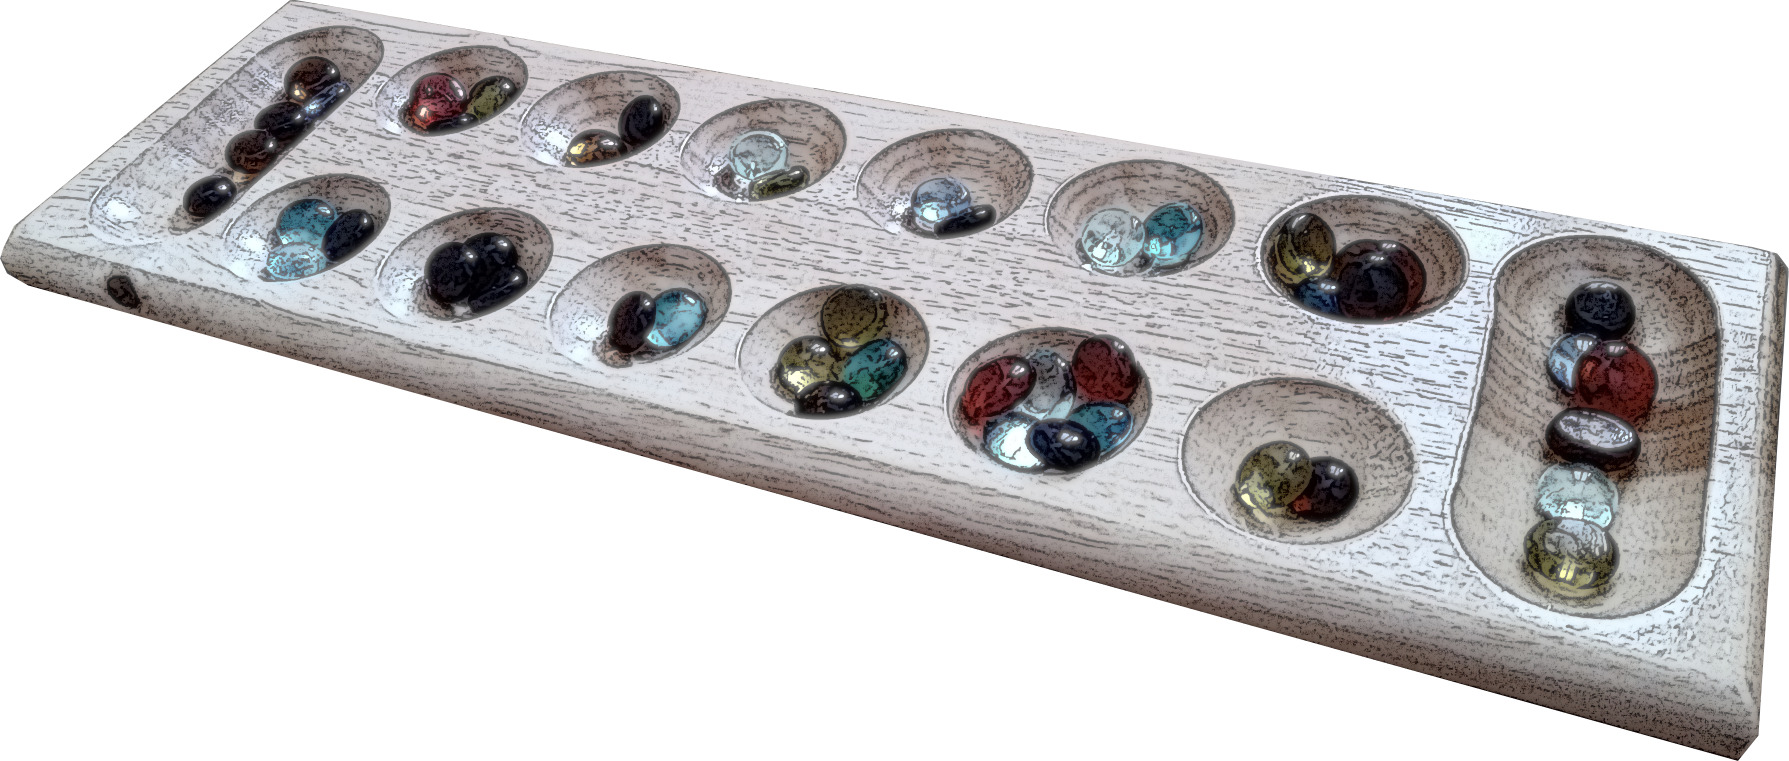
\includegraphics[width=\textwidth]{images/kalah.jpg}
\end{center}

A játéknak számos variánsa létezik, itt most egy
egyszerű változatot fogunk megvalósítani. A táblán
12 kisebb és 2 nagyobb lyuk található; az egyes
játékosokhoz a hozzájuk közelebb levő 6 lyuk és a
jobb kéz felőli nagyobb lyuk (a \emph{kalah})
tartozik. Kezdetben minden (kis) lyukban 6 kő van,
bár szokás 4--4 kővel is játszani.

A játékosok felváltva lépnek. Egy lépés abból áll,
hogy választanak egy saját lyukat, amiben van kő, és
a benne levő köveket óramutató járásával ellenkező
irányban egyesével beleszórják a következő lyukakba
-- amikor elfogynak a sajátok, akkor egy kerül a
saját kalahba, utána az ellenfél lyukaiba, és ha
azok elfogytak, akkor megint a sajátokba (az
ellenfél kalahját ki kell hagyni).

Ha az utolsó kő a (saját) kalahba esik, akkor még
egyszer lehet lépni (ez bárhányszor ismételhető). Ha
az utolsó kő egy olyan saját lyukba kerül, ami
előtte üres volt, és a szemben levő lyukban van kő,
akkor a szóró játékos mindkét lyuk tartalmát
megkapja és a kalahjába teszi.

A játékot az nyeri meg, aki megszerzi a köveknek
több, mint a felét. A játéknak akkor is vége van, ha
egy lépés végeztével az egyik térfél teljesen kiürül
-- ilyenkor a másik játékos megkapja a saját oldalán
levő köveket.

\subsection*{Keretprogram}

Ez már egy elég komplex program lesz, amit apránként
fogunk felépíteni felülről lefelé, tehát először
egy magas szinten fogalmazzuk meg, és utána
kitöltjük a részleteket.

A Kalah az absztrakt táblajátékok általános sémáját
követi; erre írhatunk egy olyan keretprogramot, ami
később akár más hasonló jellegű játékokra is
használható lesz:
\begin{program}
kalah :-
    alapbeállítás(Állás, Játékos),
    kirajzol(Állás, Játékos),
    játék(Állás, Játékos).

játék(Állás, Játékos) :-
    játék_vége(Állás, Játékos, Eredmény), !,
    bejelent(Eredmény).
játék(Állás, Játékos) :-
    lépést_választ(Állás, Játékos, Lépés),
    lép(Lépés, Állás, Állás1),
    következő_játékos(Játékos, Játékos1), !,
    kirajzol(Állás1, Játékos1),
    játék(Állás1, Játékos1).
\end{program}

Az \pr{alapbeállítás} felállítja a tábla kezdő
állapotát, és meghatározza a kezdő játékost. Ezt
az állást kirajzoljuk, és utána kezdődik a tényleges
\pr{játék/2}. Ez először ellenőrzi, hogy vége van-e
a játéknak, és ha igen, közli az
eredményt. Egyébként a soron következő játékos
választ egy lépést, ezt a lépést le is játsza, majd
a következő játékos számára kirajzolja a (módosult)
állást és a játék megy tovább.

A két játékosunk lehet az \pr{ember} és a
\pr{számítógép}, és ezek váltakoznak, tehát
\begin{program}
következő_játékos(ember, számítógép).
következő_játékos(számítógép, ember).
\end{program}

Az eredmény lehet egyszerűen a nyertes megnevezése,
vagy a \pr{döntetlen}:
\begin{program}
bejelent(ember) :- kiír('Nyertél, gratulálok!').
bejelent(számítógép) :- kiír('Nyertem.').
bejelent(döntetlen) :- kiír('Döntetlen lett!').
\end{program}

Itt a \pr{kiír} a \pr{write} olyan változata, ami
utána még egy újsort is kiír (\pr{nl}):
\begin{program}
kiír(X) :- write(X), nl.
\end{program}

\subsection*{Reprezentáció}
A legfontosabb feladat itt is, mint mindig, a
\emph{reprezentáció} (adatábrázolás) ügyes
megválasztása. Hogyan érdemes eltárolnunk az állást?
A cél, hogy később kényelmesen le tudjuk írni a
lépéseket.

Számozzuk be a lyukakat mindkét játékosnak balról
jobbra 1--6-ig. A lépés tehát mindkét játékos
számára egy 1 és 6 közötti szám lesz, vagyis
pontosabban ezeknek egy listája, ugyanis ha az
utolsó kő a kalahba kerül, akkor a játékos újra
léphet, és így egy lépést a kiválasztott lyukak
listájával lehet definiálni.

Az állást tehát a $2\times6$ lyukban, valamint a
kalahokban levő kövek számával tudjuk leírni. A
belső ábrázolásunk \pr{tábla(La, Na,Lb,Nb)} alakú
lesz, ahol \pr{La} és \pr{Lb} számok 6-elemű listája
(a lyukakban levő kövek), \pr{Na} és \pr{Nb} sima
számok (a kalahokban levő kövek). Az \pr{a}-végűek
az éppen soron következő játékoshoz tartozó adatok,
a \pr{b}-végűek az ellenfélhez tartozóak.

A játékot kezdje mindig az emberi játékos:
\begin{program}
alapbeállítás(Állás, ember) :-
    kövek_száma(K),
    Állás = tábla([K,K,K,K,K,K],0,
                  [K,K,K,K,K,K],0).

kövek_száma(6).
\end{program}

A kövek számát érdemes a fent látható módon kivenni
külön ténybe, hogy később kényelmesen változtatható
legyen.

\subsection*{A Kalah szabályai}
Mikor van vége a játéknak? Itt azt az egyszerűsítést
alkalmazhatjuk, hogy ha az egyik térfél a lépés
végére kiürül, akkor a másik térfélen levő kövek --
még a lépés részeként -- bekerülnek a megfelelő
kalahba. Elég tehát azt a feltételt megnéznünk, hogy
valamelyik játékos elvitte már a köveknek több, mint
a felét.
\begin{program}
játék_vége(tábla(_,N,_,N), _, döntetlen) :-
    kövek_száma(K), N =:= 6 * K, !.
játék_vége(tábla(_,N1,_,_), Játékos, Játékos) :-
    kövek_száma(K), N1 > 6 * K, !.
játék_vége(tábla(_,_,_,N2), Játékos, Másik) :-
    kövek_száma(K), N2 > 6 * K,
    következő_játékos(Játékos, Másik).
\end{program}

Következik a lépések leírása. Ahogy láttuk, a lépés
lyukak listájával van megadva. Ha a lista végére
értünk, akkor a másik játékos következik, ezért meg
kell ,,fordítani'' a táblát:
\begin{program}
lép([], Állás, Állás1) :- megfordít(Állás, Állás1).

megfordít(tábla(La,Na,Lb,Nb), tábla(Lb,Nb,La,Na)).
\end{program}

Egyébként pedig körbeszórjuk (,,vetjük'') a köveket:
\begin{program}
lép([L|M], Állás, Állás2) :-
    kövek(L, Állás, K),
    vet(K, L, Állás, Állás1),
    lép(M, Állás1, Állás2).
\end{program}

Itt a \pr{kövek} megadja, hogy egy adott lyukban
hány kő van:
\begin{program}
kövek(I, tábla(L,_,_,_), K) :-
    n_edik(I, L, K), K > 0.

n_edik(N, [_|M], X) :-
    N > 1, !, N1 is N - 1,
    n_edik(N1, M, X).
n_edik(1, [X|_], X).
\end{program}

A vetés a játék lelke, és egyben a legbonyolultabb
része. Ezt két részre szedjük, a saját oldalon és az
ellenfél oldalon való vetésre (utóbbi szükség
szerint újra hivatkozik majd a \pr{vet}-re):
\begin{program}
vet(Kövek, Luk, Állás, Állás2) :-
    vet_saját(Kövek, Luk, Állás, Állás1, Kövek1),
    vet_ellenfél(Kövek1, Állás1, Állás2).
\end{program}

Ez tehát azt mondja, hogy a \pr{Luk} lyukból indulva
vetünk \pr{Kövek} darab követ, és így jutunk a
kezdeti \pr{Állás}-ból a végső \pr{Állás2}-be. A
saját oldali vetés végeztekor egy közbülső
\pr{Állás1}-be jutunk, ahol még további \pr{Kövek1}
darab követ kell vetnünk az ellenfél oldalára.

Ha a kövek száma nagyobb, mint 7 $-$ \pr{Luk}, akkor
átjutunk az ellenfél oldalára (tehát az 1-es lyukból
legalább 7 kő kell, a 2-esből 6, \dots, a 6-osból
legalább 2, hiszen az első a kalahba kerül):
\begin{program}
vet_saját(Kövek, Luk, tábla(La,Na,Lb,Nb),
          tábla(La1,Na1,Lb,Nb), Kövek1) :-
    Kövek > 7 - Luk, !, % átmegy az ellenfélhez
    felvesz_és_szór(Luk, Kövek, La, La1),
    Na1 is Na + 1, Kövek1 is Kövek + Luk - 7.
\end{program}

A lényeget a \pr{felvesz\_és\_szór} végzi, amit
kicsit későbbre hagyunk. Ha nem jutunk át a másik
oldalra, akkor a megmaradó kövek száma 0:
\begin{program}
vet_saját(Kövek, Luk,
          tábla(La,Na,Lb,Nb), Állás, 0) :-
    Kövek =< 7 - Luk,
    felvesz_és_szór(Luk, Kövek, La, La1),
    elfogás(Luk, Kövek, La1, La2, Lb, Lb1, N),
    raktározás(N, Kövek, Luk, Na, Na1),
    vetés_vége(tábla(La2,Na1,Lb1,Nb), Állás).
\end{program}

Az \pr{elfogás} megnézi, hogy hány követ ejtettünk
foglyul (\pr{N}), és hogy ennek hatására hogyan
változik a tábla (új \pr{La2} és \pr{Lb1}
értékek). A \pr{raktározás} frissíti a kalah értékét
(\pr{Na1}), egyrészt az elfogott kövek, másrészt az
aktuális vetés során oda jutó kő figyelembe
vételével. Végül a \pr{vetés\_vége} ellenőrzi, hogy
kiürült-e az egyik térfél, és ha igen, akkor a
fennmaradó köveket a megfelelő kalahba teszi.

Nézzük meg ezeket sorban!
\begin{program}
elfogás(Luk, Kövek, La, La1, Lb, Lb1, N) :-
    Vége is Luk + Kövek,
    n_edik(Vége, La, 1),
    Szemben is 7 - Vége,
    n_edik(Szemben, Lb, K),
    K > 0, !, % üresbe érkeztünk és van szemben kő
    n_csere(Vége, La, 0, La1),
    n_csere(Szemben, Lb, 0, Lb1),
    N is K + 1.
elfogás(_, _, La, La, Lb, Lb, 0) :- !.

n_csere(1, [_|M], Y, [Y|M]) :- !.
n_csere(N, [X|M], Y, [X|M1]) :-
    N > 1, !, N1 is N - 1,
    n_csere(N1, M, Y, M1).
\end{program}
A \pr{Vége} adja meg, hogy melyik lyukba kerül az
utolsó kő. Ha ebben 1 kő van, tehát a vetés előtt
üres volt, akkor megvizsgáljuk, hogy szemben van-e
kő (a szemben levő lyukak számozásának iránya
fordított, ezért a megfelelő index a 7 $-$ \pr{Vége}
lesz). Ha ez is teljesül, akkor kinullázzuk ezt a
két lyukat az \pr{n\_csere(I, L, X, L1)}
használatával, ami az \pr{L} lista \pr{I}-edik
elemét \pr{X}-re állítja. Végül a kapott kövek száma
a szemben levő kövek száma + 1. Ellenkező esetben a
tábla változatlan marad és a kapott kövek száma 0
lesz.

Figyeljük meg, hogy itt az aránylag bonyolult
feltételt nem ismételjük meg a második szabályban,
hanem a procedurális olvasatra hagyatkozunk: az első
szabályban levő vágás miatt a másodikba csak akkor
jutunk, ha a feltétel nem teljesül. Ez a deklaratív
olvasatot elrontja, de megengedhető, mivel tudjuk,
hogy csak olyan környezetben használjuk, ahol az
\pr{La1}, \pr{Lb1} és \pr{N} változóknak nincsen
értéke. A hatékonyság érdekében sok szabály
használja itt ezt a módszert.

A \pr{raktározás} elég magától értetődő. Ha az
elfogott kövek száma 0, akkor ellenőrzi, hogy az
utolsó kő a kalahba került-e, egyébként csak
hozzáadja az eddigiekhez az elfogott köveket:
\begin{program}
raktározás(0, Kövek, Luk, Na, Na) :-
    Kövek < 7 - Luk, !.
raktározás(0, Kövek, Luk, Na, Na1) :-
    Kövek =:= 7 - Luk, !, Na1 is Na + 1.
raktározás(N, _, _, Na, Na1) :-
    N > 0, !, Na1 is Na + N.
\end{program}

A kiürült térfelek kezelésekor a másik térfél köveit
összeadjuk, és azt is kiürítjük:
\begin{program}
vetés_vége(tábla(La,Na,Lb,Nb),
           tábla(La,Na,La,Nb1)) :-
    üres(La), !, összeg(Lb, X), Nb1 is Nb + X.
vetés_vége(tábla(La,Na,Lb,Nb),
           tábla(Lb,Na1,Lb,Nb)) :-
    üres(Lb), !, összeg(La, X), Na1 is Na + X.
vetés_vége(Állás, Állás) :- !.

üres([0,0,0,0,0,0]).

összeg(L, X) :- összeg(L, 0, X).

összeg([], A, A).
összeg([K|M], A, X) :-
    A1 is A + K,
    összeg(M, A1, X).
\end{program}

A saját oldali vetéssel így már majdnem készen
vagyunk, csak a \pr{felvesz\_és\_szór} hiányzik:
\begin{program}
felvesz_és_szór(0, K, L, L1) :- % szórás folytatása
    !, szór(K, L, L1).
felvesz_és_szór(1, K, [_|M], [0|M1]) :-
    !, szór(K, M, M1).
felvesz_és_szór(Luk, K, [L|M], [L|M1]) :-
    Luk > 1, !, Luk1 is Luk - 1,
    felvesz_és_szór(Luk1, K, M, M1).
\end{program}

A \pr{K} itt a szórandó kövek számát adja meg, a
\pr{Luk} pedig a lyuknak a száma, ahonnan
szórunk. Ha a \pr{Luk} értéke 0, az azt jelenti,
hogy egy korábban elkezdődött vetés folytatódik, és
az első kőnek az 1-es számú lyukba kell esnie. (A
tényleges szórást a \pr{szór} végzi.) Ha a \pr{Luk}
száma az 1-es, akkor a kapott lyuk-lista első elemét
kinullázzuk (kivesszük belőle a köveket), a többit
pedig a \pr{szór} segítségével módosítjuk. Végül ha
a \pr{Luk} száma nagyobb, mint 1, akkor a lyuk-lista
első eleme megmarad, a maradékot pedig rekurzív
hívással tudjuk megadni.

A szórásnál lyukanként haladunk, és mindegyikbe egy
kő kerül, amíg vagy nincs több lyuk, vagy nincs több kő:
\begin{program}
szór(0, L, L) :- !.
szór(N, [L|M], [L1|M1]) :-
    N > 0, !,
    N1 is N - 1, L1 is L + 1,
    szór(N1, M, M1).
szór(_, [], []) :- !.
\end{program}

Hátra van még a vetés az ellenfél oldalán. Itt 4
esetet különböztetünk meg:
\begin{enumerate}
\item A vetni való kövek száma 0. Ilyenkor nincs
  teendő.
\item A kövek száma 1 és 6 között van (tehát nem jön
  vissza hozzánk), és a mi térfelünk nem
  üres. Ilyenkor egyszerűen végig kell szórni ezeket
  a köveket.
\item A kövek száma 1 és 6 között van, és a saját
  térfél üres. Ilyenkor az ellenfél kalahjába
  bekerülnek a szórandó kövek és az ellenfél
  térfelén levők is.
\item A kövek száma több, mint 6. Ekkor a kövek
  végigszórása után 6-al kevesebb kővel egy újabb
  vetést kell indítani a saját térfél ,,0-dik''
  lyukából.
\end{enumerate}

Ennek megfelel az alábbi 4 szabály:
\begin{program}
vet_ellenfél(0, Állás, Állás) :- !.
vet_ellenfél(Kövek, tábla(La,Na,Lb,Nb),
             tábla(La,Na,Lb1,Nb)) :-
    1 =< Kövek, Kövek =< 6,
    \+ üres(La), !,
    szór(Kövek, Lb, Lb1).
vet_ellenfél(Kövek, tábla(La,Na,Lb,Nb),
             tábla(La,Na,La,Nb1)) :-
    1 =< Kövek, Kövek =< 6,
    üres(La), !,
    összeg(Lb, X), Nb1 is Nb + Kövek + X.
vet_ellenfél(Kövek, tábla(La,Na,Lb,Nb), Állás) :-
    Kövek > 6, !,
    szór(6, Lb, Lb1),
    Kövek1 is Kövek - 6,
    vet(Kövek1, 0, tábla(La,Na,Lb1,Nb), Állás).
\end{program}

\subsection*{Kirajzolás}
A nehezén túl vagyunk, de ahhoz, hogy játszani is
tudjunk, meg is kell valahogy jeleníteni a táblát,
és kommunikálni kell a játékossal.

A tábla így fog kinézni:
\begin{query}
     6    6    6    6    6    6
0                                  0
     6    6    6    6    6    6
\end{query}

A kirajzolásnál mindig a(z ember) játékos sora lesz
alul, tehát a számítógép sorát kell elsőnek
kiírni. Ezt úgy érjük el, hogy ha a játékos jön,
akkor megfordítjuk a táblát a tényleges kirajzolás
előtt:
\begin{program}
kirajzol(Állás, számítógép) :- kirajzol(Állás).
kirajzol(Állás, ember) :-
    megfordít(Állás, Állás1),
    kirajzol(Állás1).
\end{program}

A két sor kiírását a \pr{sort\_ír} végzi, a
kalahokét a \pr{kalahot\_ír}. A felső sor számozása
jobbról balra történik, tehát ezt a listát meg kell
fordítani kiírás előtt:
\begin{program}
kirajzol(tábla(La,Na,Lb,Nb)) :-
    nl,
    fordított(La, F),
    sort_ír(F),
    kalahot_ír(Na, Nb),
    sort_ír(Lb).
\end{program}

A sorokat 5 szóköznyi behúzással indítjuk, hogy
legyen hely a baloldali kalahnak is:
\begin{program}
sort_ír(L) :- behúz(5), lyukat_ír(L).

lyukat_ír([]) :- nl.
lyukat_ír([L|M]) :- köveket_ír(L), lyukat_ír(M).

köveket_ír(N) :- N < 10, write(N), behúz(4).
köveket_ír(N) :- N >= 10, write(N), behúz(3).

kalahot_ír(N1, N2) :-
    köveket_ír(N1), behúz(30),
    write(N2), nl.

behúz(0) :- !.
behúz(N) :-
    N > 0, N1 is N - 1,
    write(' '), behúz(N1).
\end{program}

A \pr{köveket\_ír} mindig 3 vagy 4 szóközt ír annak
függvényében, hogy egy- vagy kétjegyű a kövek száma.

\subsection*{Próba kétjátékosos módban}
A mesterséges intelligencia még nincs meg, de a
program már majdnem tesztelhető. Csak a
\pr{lépést\_választ} hiányzik, amit egyelőre írjunk
meg úgy, hogy mindig a játékost kérdezi:
\begin{program}
lépést_választ(_, _, Lépés) :-
    nl, kiír('Melyiket választod?'),
    read(Lépés), érvényes(Lépés).

érvényes([]).
érvényes([L|M]) :- 0 < L, L < 7, érvényes(M).
\end{program}

A lépés érvényességére csak egy minimális ellenőrzés
van, azt sem ellenőrzi, hogy nem kéne-e folytatnunk
a lépést vagy hogy nem léptünk-e túl sokszor.

Itt egy pár lépés ízelítőnek:
\begin{query}
?- kalah.

     6    6    6    6    6    6
0                                  0
     6    6    6    6    6    6

Melyiket választod?
|: [1,5].

     6    7    7    7    7    7
0                                  2
     0    7    7    7    0    8

Melyiket választod?
|: [3].

     7    8    8    0    7    7
1                                  2
     1    8    8    7    0    8

Melyiket választod?
|: [2].

     7    8    8    1    8    8
1                                  3
     1    0    9    8    1    9

Melyiket választod?
|: [1].

     8    9    9    2    9    0
2                                  3
     2    1    9    8    1    9

Melyiket választod?
|: [6].

     9    10   10   3    10   1
2                                  4
     3    2    9    8    1    0

Melyiket választod?
|: [3].

     10   11   11   0    10   1
2                                  4
     3    2    9    8    1    0

Melyiket választod?
|: [5].

     10   11   11   0    10   0
2                                  6
     3    2    9    8    0    0

Melyiket választod?
|: vége.

false.
\end{query}

A program jelenleg tetszőleges hibás lépésre
(pl. \pr{vége}) leáll. Kipróbálhatjuk egy-egy
speciális esetre is, mint például ez:
\begin{query}
?- Állás = tábla([1,1,1,1,1,1],23,[16,3,1,1,3,3],16),
   kirajzol(Állás, ember), játék(Állás, ember).

     3    3    1    1    3    16
16                                  23
     1    1    1    1    1    1

Melyiket választod?
|: [6,5].

     3    3    1    1    3    0
16                                  41
     1    1    1    1    0    0
Nyertél, gratulálok!
\end{query}

\subsection*{Alfa--béta nyírás keretprogram}
A számítógép az ún.~\emph{alfa--béta nyírás}
algoritmusa szerint fog működni. Ennek a lényege az,
hogy minden játékálláshoz tudunk rendelni egy
számot, ami annál magasabb, minél kedvezőbb
nekünk az állás. Ezután végiggondoljuk az összes lépési
lehetőséget (az ellenfél lépéseit is természetesen)
valahány lépésre előre: ezt a lépésszámot szokás
\emph{mélységnek} nevezni, a programban az
\emph{előrelátás} rövidítéseként az \pr{E} betűt
fogjuk rá alkalmazni.
\index{alfa--béta nyírás}

Nézzünk egy nagyon egyszerű példát! Az alábbi ábra
lépések \emph{fáját} mutatja: a pontok és számok
játékállásokat jelölnek, míg a köztük levő szakaszok
a lépéseket.

\begin{center}
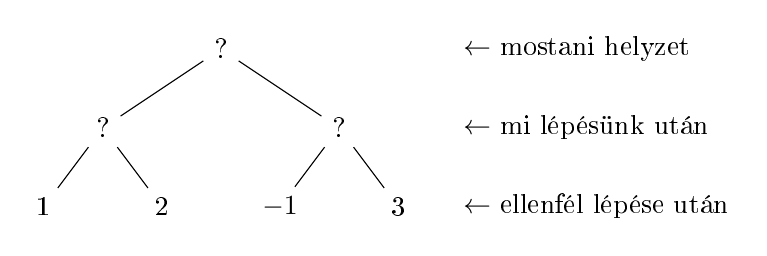
\begin{tikzpicture}[level distance=1cm,
    level 1/.style={sibling distance=3cm},
    level 2/.style={sibling distance=1.5cm}]
  \node (Root) {?}
  child {
    node {?}
    child { node {1} }
    child { node {2} }
  }
  child {
    node {?}
    child { node {$-1$} }
    child { node {3} }
  };
  \begin{scope}[every node/.style={right}]
    \path (Root    -| Root-2-2) node {$\qquad\leftarrow$ mostani helyzet};
    \path (Root-1  -| Root-2-2) node {$\qquad\leftarrow$ mi lépésünk után};
    \path (Root-1-1-| Root-2-2) node {$\qquad\leftarrow$ ellenfél lépése után};
  \end{scope}
\end{tikzpicture}
\end{center}

Itt a mélység 2, tehát 2 lépésre előre gondolkodunk,
és a legmélyebb szinten kiértékelünk minden
állást. Két lépéslehetőségünk van, és ezekre az
ellenfélnek 2-2 válasza. Feltesszük, hogy az
ellenfelünk jól játszik, tehát ha a baloldali lépést
választjuk, arra az ellenfél a saját baloldali (1-es
értékelésű) lépését fogja válaszolni, nem pedig a
jobboldalit, ami nekünk kedvezőbb állást (2)
eredményez. Hasonlóan járunk el a jobboldali
lépésnél: az ellenfél két válasza közül
feltételezzük a kisebbet (-1). Azt láttuk tehát,
hogy a baloldali lépés legrosszabb esetben 1-es, a
jobboldali -1-es értékelésű. Mi nyilván a nagyobbat
választjuk, tehát a mostani helyzetünk 1-es
értékelésű lesz:

\begin{center}
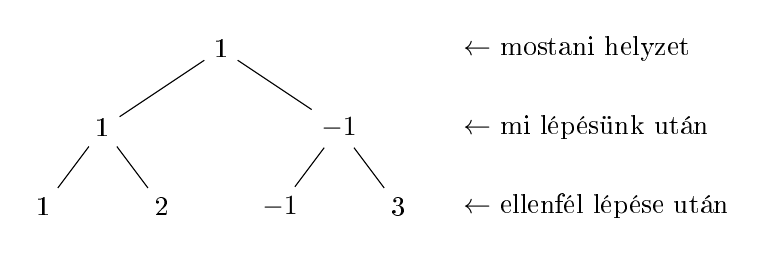
\begin{tikzpicture}[level distance=1cm,
    level 1/.style={sibling distance=3cm},
    level 2/.style={sibling distance=1.5cm}]
  \node (Root) {1}
  child {
    node {1}
    child { node {1} }
    child { node {2} }
  }
  child {
    node {$-1$}
    child { node {$-1$} }
    child { node {3} }
  };
  \begin{scope}[every node/.style={right}]
    \path (Root    -| Root-2-2) node {$\qquad\leftarrow$ mostani helyzet};
    \path (Root-1  -| Root-2-2) node {$\qquad\leftarrow$ mi lépésünk után};
    \path (Root-1-1-| Root-2-2) node {$\qquad\leftarrow$ ellenfél lépése után};
  \end{scope}
\end{tikzpicture}
\end{center}

Ha itt kell lépést választani, akkor a baloldali
mellett döntünk. Ezt a gondolkodást \emph{minimax}
algoritmusnak hívják, mivel az ellenfél lépései
közül a minimális értékűt, a saját lépések közül a
maximális értékűt választjuk.
\index{minimax}

Az alfa--béta nyírás ennek egy hatékonyabb
változata. Itt mindig számon tartjuk azt, hogy mi az
a minimum, amit biztosan el tudunk érni ($\alpha$, a
programban \pr{A}), és mi az a maximum, amit
elérhetünk ($\beta$, a programban \pr{B}), ezek
adják a módszer nevét. Nézzük meg az előbbi példa
kiértékelését, amikor már megvizsgáltuk a teljes
baloldali ágat!

\begin{center}
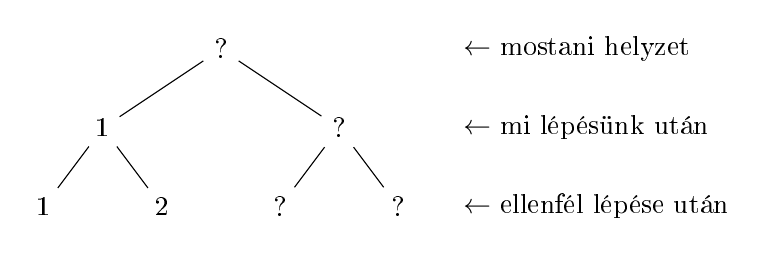
\begin{tikzpicture}[level distance=1cm,
    level 1/.style={sibling distance=3cm},
    level 2/.style={sibling distance=1.5cm}]
  \node (Root) {?}
  child {
    node {1}
    child { node {1} }
    child { node {2} }
  }
  child {
    node {?}
    child { node {?} }
    child { node {?} }
  };
  \begin{scope}[every node/.style={right}]
    \path (Root    -| Root-2-2) node {$\qquad\leftarrow$ mostani helyzet};
    \path (Root-1  -| Root-2-2) node {$\qquad\leftarrow$ mi lépésünk után};
    \path (Root-1-1-| Root-2-2) node {$\qquad\leftarrow$ ellenfél lépése után};
  \end{scope}
\end{tikzpicture}
\end{center}

A jobboldali ággal még egyáltalán nem
foglalkoztunk. Azt tudjuk, hogy ha a baloldali
lépést választjuk, legrosszabb esetben 1-es (tehát
$\alpha=1$). Hogyan módosul ez a jobboldali lépésre
adott baloldali válasz megvizsgálása után?

\begin{center}
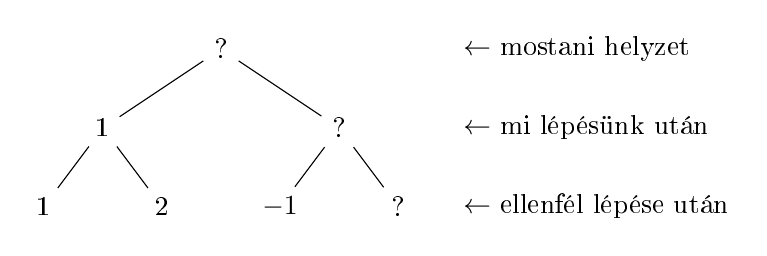
\begin{tikzpicture}[level distance=1cm,
    level 1/.style={sibling distance=3cm},
    level 2/.style={sibling distance=1.5cm}]
  \node (Root) {?}
  child {
    node {1}
    child { node {1} }
    child { node {2} }
  }
  child {
    node {?}
    child { node {$-1$} }
    child { node {?} }
  };
  \begin{scope}[every node/.style={right}]
    \path (Root    -| Root-2-2) node {$\qquad\leftarrow$ mostani helyzet};
    \path (Root-1  -| Root-2-2) node {$\qquad\leftarrow$ mi lépésünk után};
    \path (Root-1-1-| Root-2-2) node {$\qquad\leftarrow$ ellenfél lépése után};
  \end{scope}
\end{tikzpicture}
\end{center}

Azt látjuk, hogy ha a jobboldali lépést választjuk,
akkor legjobb esetben -1-re számíthatunk
($\beta=-1$). Lehet, hogy az ellenfélnek van egy még
erősebb lépése, és a tényleges maximum még kisebb,
de nagyobb nem lehet. Viszont a baloldali ágon már
van egy biztos 1-es, tehát ezt az ágat nem érdemes
tovább vizsgálni, le lehet ,,nyírni''. Általában
tehát ha egy ágon a $\beta$ érték kisebb vagy
egyenlő, mint az eddigi legjobb $\alpha$, akkor nem
kell vele foglalkozni.

Az algoritmust teljesen általánosan meg lehet
fogalmazni, a konkrét játéktól függetlenül. Csak azt
feltételezzük, hogy a következők adottak:
\begin{itemize}
\item \pr{lépés(Állás, Lépés)} : adott állásból
  lehetséges lépés
\item \pr{lép(Lépés, Állás, Állás1)} : adott lépés
  lejátszása
\item \pr{értékelés(Állás, Érték)} : adott állás
  kiértékelése
\end{itemize}

Ebből egyelőre csak a második van meg, a maradék
kettőt a következő részben fogjuk elkészíteni. Most
azonban nézzük az általános algoritmust! Hogy ne
kelljen külön kezelni a minimum- és maximumkereső
eseteket, az értékeléseket minden szintváltáskor
negáljuk. Ahhoz, hogy ez működjön, feltételezzük,
hogy a keresési mélység kezdetben páros, tehát a
0-ás mélységen a pozitív szám jelenti a nekünk jó
állást.

\begin{program}
alfa_béta(0, Állás, _, _, _-Érték) :-
    értékelés(Állás, Érték).
alfa_béta(E, Állás, A, B, Lépés-Érték) :-
    E > 0, E1 is E - 1,
    A1 is -B, B1 is -A,
    findall(L, lépés(Állás, L), Lépések),
    választ(Lépések, Állás, E1, A1, B1,
            nincs, Lépés-Érték).
\end{program}

Ha az előrelátás mélysége 0, akkor az aktuális
állást egyszerűen kiértékeljük. (Ilyenkor a legjobb
lépést jelölő \pr{Lépés} nem kap értéket.) Ha a
mélység legalább 1, akkor eggyel csökkentjük,
negáljuk és megcseréljük az alfát és bétát (hogy a
másik játékos szemszögébe kerüljünk), és választunk
az összes lehetséges lépés közül.

A választást a \pr{választ} végzi:
\begin{program}
választ([], _, _, A, _, Legjobb, Legjobb-A).
választ([Lépés|M], Állás, E, A, B, Legjobb, X) :-
    lép(Lépés, Állás, Állás1),
    alfa_béta(E, Állás1, A, B, _-Érték),
    Érték1 is -Érték,
    nyír(Lépés-Érték1, E, A, B, M, Állás,
         Legjobb, X).
\end{program}

Az utolsóelőtti argumentum az eddigi legjobb lépés
(kezdetben \pr{nincs}), az utolsó pedig a végső
megtalált legjobb lépés és a hozzá tartozó
értékelés.

Ha a lehetséges lépések listája üres, akkor az
eddigi legjobb lépést adja vissza (\pr{Legjobb}) és
a hozzá tartozó érték az \pr{A} lesz. Ha nem
üres, akkor kipróbálja az első lépést: lejátsza, és
az így keletkező állást (rekurzívan) kiértékeli az
\pr{alfa\_béta} szabállyal. Az így kapott
\pr{Érték}-et negálni kell, mert egy szinttel
feljebb léptünk. Végül a \pr{nyír} az eredeti
\pr{Állás} állapotból való lépések közül
(rekurzívan) választ, miközben lenyírja azokat az
ágakat, amelyeket felesleges kiértékelni:
\begin{program}
nyír(Lépés-Érték, _, _, B, _, _, _, Lépés-Érték) :-
    Érték >= B.
nyír(Lépés-Érték, E, A, B, Többi, Állás, _, X) :-
    A < Érték, Érték < B,
    választ(Többi, Állás, E, Érték, B, Lépés, X).
nyír(_-Érték, E, A, B, Többi, Állás, Lépés1, X) :-
    Érték =< A,
    választ(Többi, Állás, E, A, B, Lépés1, X).
\end{program}

Itt három esetet különböztetünk meg, a megvizsgált
lépés értékelésétől függően:
\begin{enumerate}
\item Ha legalább $\beta$, akkor nem kell tovább
  keresni, ennél jobb lépés nem változtat az
  értékelésen. (Ez megfelel annak, hogy a fenti
  példában megtaláltuk a $-1$-et, ami az ellenfél
  számára negálva 1-es, és ezért nem kell még jobb
  lépés után néznie, mert a $\beta$ (a mi negált
  $\alpha$-nk) kisebb, $-1$ értékű.)
\item Ha $\alpha$ és $\beta$ között van, akkor ez
  lesz az eddigi legjobb lépés és az értéke az új
  $\alpha$, és keresünk egy esetleges jobbat a többi
  lépésből.
\item Ha kisebb vagy egyenlő, mint $\alpha$, akkor
  ez a lépés nem érdekes, a többiekben folytatjuk a
  keresést.
\end{enumerate}

\subsection*{Kalah-specifikus részek}
Hogyan tudjuk az összes lehetséges lépést leírni?
\begin{program}
lépés(tábla([0,0,0,0,0,0],_,_,_), []).
lépés(Állás, [L|M]) :-
    tartalmaz(L, [1,2,3,4,5,6]),
    kövek(L, Állás, K),
    lépést_folytat(K, L, Állás, M).
\end{program}
Ha a térfelünk üres, nincs lehetséges lépés. (Erre
azért van szükség, mert a játékot be lehet fejezni
úgy, hogy az utolsó követ a kalahba rakjuk.)
Egyébként a lépés első eleme egy lyukat jelölő 1 és
6 közti szám; a \pr{kövek} biztosítja, hogy van is
benne kő. Azt kell csak ellenőrizni, hogy a kalahba
kerül-e az utolsó, amire a feltétel a 13-al való
osztási maradékkal számolható:
\begin{program}
lépést_folytat(Kövek, L, _, []) :-
    Kövek =\= (7 - L) mod 13, !.
lépést_folytat(Kövek, L, Állás, Lépések) :-
    Kövek =:= (7 - L) mod 13, !,
    vet(Kövek, L, Állás, Állás1),
    lépés(Állás1, Lépések).
\end{program}
Ha a kalahba került, akkor a köveket végigszórjuk,
és ebből az állásból rekurzívan további lépéseket
keresünk.

Egy állás értékelésére egy nagyon egyszerű definíció
a kalahokban levő kövek különbsége:
\begin{program}
értékelés(tábla(_,Na,_,Nb), X) :- X is Na - Nb.
\end{program}

Már csak annyi van hátra, hogy átírjuk a
\pr{lépést\_választ} szabályt. A régi verzió
megmarad arra az esetre, amikor az emberi játékos
van lépésen; a számítógép esetében pedig az
alfa--béta nyírást használjuk:
\begin{program}
lépést_választ(_, ember, Lépés) :-
    nl, kiír('Melyiket választod?'),
    read(Lépés), érvényes(Lépés).
lépést_választ(Állás, számítógép, Lépés) :-
    előrelátás(E),
    alfa_béta(E, Állás, -40, 40, Lépés-_),
    nl, write(Lépés), nl.

előrelátás(4).
\end{program}

Az $[\alpha,\beta]$ intervallumot kezdetben jó
nagyra állítjuk (-40, 40), az előrelátás mélységét
pedig a könnyebb módosíthatóság kedvéért egy külön
tényként tároljuk.

\subsection*{Tesztjáték}
Itt egy 6-os mélységű mesterséges intelligencia
ellen játszott 4-köves játék, ahol a gép kezdett:
\begin{query}
?- kalah.

     4    4    4    4    4    4
0                                  0
     4    4    4    4    4    4

[3,6]

     0    5    5    0    4    4
2                                  0
     5    5    5    5    4    4

Melyiket választod?
|: [2,1].

     0    5    5    0    4    4
2                                  1
     0    1    7    7    6    6

[4]

     1    6    0    0    4    4
3                                  1
     1    2    7    7    6    6

Melyiket választod?
|: [1].

     1    6    0    0    4    4
3                                  1
     0    3    7    7    6    6

[5]

     2    0    0    0    4    4
4                                  1
     1    4    8    8    6    6

Melyiket választod?
|: [2].


     2    0    0    0    4    4
4                                  1
     1    0    9    9    7    7

[6]

     0    0    0    0    4    4
5                                  1
     2    0    9    9    7    7

Melyiket választod?
|: [1].

     0    0    0    0    4    4
5                                  1
     0    1    10   9    7    7

[1]

     0    0    1    1    5    0
7                                  1
     0    0    10   9    7    7

Melyiket választod?
|: [5].

     0    1    2    2    6    1
7                                  2
     0    0    10   9    0    8

[1]

     0    1    2    2    7    0
7                                  2
     0    0    10   9    0    8

Melyiket választod?
|: [6].

     0    2    3    3    8    1
7                                  5
     0    0    10   9    0    0

[5,6,4,6,1]

     0    1    0    3    9    0
11                                 5
     0    0    10   9    0    0

Melyiket választod?
|: [3].

     1    2    1    4    10   1
11                                 6
     0    0    0    10   1    1

[6,5,4]

     1    1    0    4    10   1
13                                 6
     0    0    0    10   1    1

Melyiket választod?
|: [4].

     0    2    1    5    11   2
13                                 10
     0    0    0    0    2    2

[1]

     0    2    1    6    12   0
13                                 10
     0    0    0    0    2    2

Melyiket választod?
|: [6].

     0    2    1    6    12   1
13                                 11
     0    0    0    0    2    0

[1]

     0    2    1    6    13   0
13                                 11
     0    0    0    0    2    0

Melyiket választod?
|: [5,6].

     0    0    0    0    0    0
35                                 13
     0    0    0    0    0    0
Nyertem.
\end{query}

\begin{problem}
Írd át a játékos lépését, hogy hibás lépés
esetén kérdezzen újra, és \pr{kilépés}-re lépjen ki!
\end{problem}
\begin{problem}
Készíts szigorúbb ellenőrzést az emberi játékos
lépéseihez, ami (i) nem enged üres lyukat
választani, és (ii) akkor és csak akkor enged több
lépést, ha az utolsó kő a kalahba kerül!
\end{problem}
\begin{problem}
Írd át a programot úgy, hogy a bonyolultabb (de
izgalmasabb) Oware játék szabályait kövesse!  A
különbségek:
\begin{itemize}
\item A kövek száma általában lyukanként 4
\item A szórásnál a kalahokat és a kezdő lyukat ki kell hagyni
\item Követ úgy lehet szerezni, hogy ha olyan helyre
  érkezünk, ami (i) az ellenfél oldalán van és (ii)
  a szórás befejeztével 2 vagy 3 kő lesz benne.  Ha
  ez teljesül, akkor az ebben levő összes követ
  megkapjuk, sőt, ha az előzőre is teljesül, akkor
  az abban levőket is és így tovább, amíg igaz a két
  feltétel.
\item Ha lehet, muszáj olyat lépnünk, hogy az
  ellenfél oldalán maradjon kő. Ha nem lehet, akkor
  a maradék köveket megkapjuk.
\end{itemize}
\end{problem}
\begin{problem}
Írj dámajátékot! A játék kerete legyen ugyanaz,
és a számítógép használja a fenti alfa--béta nyírás
algoritmust.
\end{problem}

\subsection*{A teljes program}
\begin{program}
% Magas szintű keretprogram

kalah :-
    alapbeállítás(Állás, Játékos),
    kirajzol(Állás, Játékos),
    játék(Állás, Játékos).

játék(Állás, Játékos) :-
    játék_vége(Állás, Játékos, Eredmény), !,
    bejelent(Eredmény).
játék(Állás, Játékos) :-
    lépést_választ(Állás, Játékos, Lépés),
    lép(Lépés, Állás, Állás1),
    következő_játékos(Játékos, Játékos1), !,
    kirajzol(Állás1, Játékos1),
    játék(Állás1, Játékos1).

következő_játékos(ember, számítógép).
következő_játékos(számítógép, ember).

bejelent(ember) :- kiír('Nyertél, gratulálok!').
bejelent(számítógép) :- kiír('Nyertem.').
bejelent(döntetlen) :- kiír('Döntetlen lett!').

% Reprezentáció

alapbeállítás(Állás, ember) :-
    kövek_száma(K),
    Állás = tábla([K,K,K,K,K,K],0,
                  [K,K,K,K,K,K],0).

% Szabályok

játék_vége(tábla(_,N,_,N), _, döntetlen) :-
    kövek_száma(K), N =:= 6 * K, !.
játék_vége(tábla(_,N1,_,_), Játékos, Játékos) :-
    kövek_száma(K), N1 > 6 * K, !.
játék_vége(tábla(_,_,_,N2), Játékos, Másik) :-
    kövek_száma(K), N2 > 6 * K,
    következő_játékos(Játékos, Másik).

lép([], Állás, Állás1) :- megfordít(Állás, Állás1).
lép([L|M], Állás, Állás2) :-
    kövek(L, Állás, K),
    vet(K, L, Állás, Állás1),
    lép(M, Állás1, Állás2).

megfordít(tábla(La,Na,Lb,Nb), tábla(Lb,Nb,La,Na)).

kövek(I, tábla(L,_,_,_), K) :- n_edik(I, L, K), K > 0.

vet(Kövek, Luk, Állás, Állás2) :-
    vet_saját(Kövek, Luk, Állás, Állás1, Kövek1),
    vet_ellenfél(Kövek1, Állás1, Állás2).

vet_saját(Kövek, Luk, tábla(La,Na,Lb,Nb),
          tábla(La1,Na1,Lb,Nb), Kövek1) :-
    Kövek > 7 - Luk, !, % átmegy az ellenfélhez
    felvesz_és_szór(Luk, Kövek, La, La1),
    Na1 is Na + 1, Kövek1 is Kövek + Luk - 7.
vet_saját(Kövek, Luk,
          tábla(La,Na,Lb,Nb), Állás, 0) :-
    Kövek =< 7 - Luk,
    felvesz_és_szór(Luk, Kövek, La, La1),
    elfogás(Luk, Kövek, La1, La2, Lb, Lb1, N),
    raktározás(N, Kövek, Luk, Na, Na1),
    vetés_vége(tábla(La2,Na1,Lb1,Nb), Állás).

felvesz_és_szór(0, K, L, L1) :- % szórás folytatása
    !, szór(K, L, L1).
felvesz_és_szór(1, K, [_|M], [0|M1]) :-
    !, szór(K, M, M1).
felvesz_és_szór(Luk, K, [L|M], [L|M1]) :-
    Luk > 1, !, Luk1 is Luk - 1,
    felvesz_és_szór(Luk1, K, M, M1).

szór(0, L, L) :- !.
szór(N, [L|M], [L1|M1]) :-
    N > 0, !,
    N1 is N - 1, L1 is L + 1,
    szór(N1, M, M1).
szór(_, [], []) :- !.

elfogás(Luk, Kövek, La, La1, Lb, Lb1, N) :-
    Vége is Luk + Kövek,
    n_edik(Vége, La, 1),
    Szemben is 7 - Vége,
    n_edik(Szemben, Lb, K),
    K > 0, !, % üresbe érkeztünk és van szemben kő
    n_csere(Vége, La, 0, La1),
    n_csere(Szemben, Lb, 0, Lb1),
    N is K + 1.
elfogás(_, _, La, La, Lb, Lb, 0) :- !.

raktározás(0, Kövek, Luk, Na, Na) :-
    Kövek < 7 - Luk, !.
raktározás(0, Kövek, Luk, Na, Na1) :-
    Kövek =:= 7 - Luk, !, Na1 is Na + 1.
raktározás(N, _, _, Na, Na1) :-
    N > 0, !, Na1 is Na + N.

vetés_vége(tábla(La,Na,Lb,Nb),
           tábla(La,Na,La,Nb1)) :-
    üres(La), !, összeg(Lb, X), Nb1 is Nb + X.
vetés_vége(tábla(La,Na,Lb,Nb),
           tábla(Lb,Na1,Lb,Nb)) :-
    üres(Lb), !, összeg(La, X), Na1 is Na + X.
vetés_vége(Állás, Állás) :- !.

üres([0,0,0,0,0,0]).

vet_ellenfél(0, Állás, Állás) :- !.
vet_ellenfél(Kövek, tábla(La,Na,Lb,Nb),
             tábla(La,Na,Lb1,Nb)) :-
    1 =< Kövek, Kövek =< 6,
    \+ üres(La), !,
    szór(Kövek, Lb, Lb1).
vet_ellenfél(Kövek, tábla(La,Na,Lb,Nb),
             tábla(La,Na,La,Nb1)) :-
    1 =< Kövek, Kövek =< 6,
    üres(La), !,
    összeg(Lb, X), Nb1 is Nb + Kövek + X.
vet_ellenfél(Kövek, tábla(La,Na,Lb,Nb), Állás) :-
    Kövek > 6, !,
    szór(6, Lb, Lb1),
    Kövek1 is Kövek - 6,
    vet(Kövek1, 0, tábla(La,Na,Lb1,Nb), Állás).

% Kirajzolás

kirajzol(Állás, számítógép) :- kirajzol(Állás).
kirajzol(Állás, ember) :-
    megfordít(Állás, Állás1),
    kirajzol(Állás1).

kirajzol(tábla(La,Na,Lb,Nb)) :-
    nl,
    fordított(La, F),
    sort_ír(F),
    kalahot_ír(Na, Nb),
    sort_ír(Lb).

sort_ír(L) :- behúz(5), lyukat_ír(L).

lyukat_ír([]) :- nl.
lyukat_ír([L|M]) :- köveket_ír(L), lyukat_ír(M).

köveket_ír(N) :- N < 10, write(N), behúz(4).
köveket_ír(N) :- N >= 10, write(N), behúz(3).

kalahot_ír(N1, N2) :-
    köveket_ír(N1), behúz(30),
    write(N2), nl.

% Alfa-béta nyírás

alfa_béta(0, Állás, _, _, _-Érték) :-
    értékelés(Állás, Érték).
alfa_béta(E, Állás, A, B, Lépés-Érték) :-
    E > 0, E1 is E - 1,
    A1 is -B, B1 is -A,
    findall(L, lépés(Állás, L), Lépések),
    választ(Lépések, Állás, E1, A1, B1,
            nincs, Lépés-Érték).

választ([], _, _, A, _, Legjobb, Legjobb-A).
választ([Lépés|M], Állás, E, A, B, Legjobb, X) :-
    lép(Lépés, Állás, Állás1),
    alfa_béta(E, Állás1, A, B, _-Érték),
    Érték1 is -Érték,
    nyír(Lépés-Érték1, E, A, B, M, Állás,
         Legjobb, X).

nyír(Lépés-Érték, _, _, B, _, _, _, Lépés-Érték) :-
    Érték >= B.
nyír(Lépés-Érték, E, A, B, Többi, Állás, _, X) :-
    A < Érték, Érték < B,
    választ(Többi, Állás, E, Érték, B, Lépés, X).
nyír(_-Érték, E, A, B, Többi, Állás, Lépés1, X) :-
    Érték =< A,
    választ(Többi, Állás, E, A, B, Lépés1, X).

% Kalah-specifikus rész

lépés(tábla([0,0,0,0,0,0],_,_,_), []).
lépés(Állás, [L|M]) :-
    tartalmaz(L, [1,2,3,4,5,6]),
    kövek(L, Állás, K),
    lépést_folytat(K, L, Állás, M).

lépést_folytat(Kövek, L, _, []) :-
    Kövek =\= (7 - L) mod 13, !.
lépést_folytat(Kövek, L, Állás, Lépések) :-
    Kövek =:= (7 - L) mod 13, !,
    vet(Kövek, L, Állás, Állás1),
    lépés(Állás1, Lépések).

értékelés(tábla(_,Na,_,Nb), X) :- X is Na - Nb.

lépést_választ(_, ember, Lépés) :-
    nl, kiír('Melyiket választod?'),
    read(Lépés), érvényes(Lépés).
lépést_választ(Állás, számítógép, Lépés) :-
    előrelátás(E),
    alfa_béta(E, Állás, -40, 40, Lépés-_),
    nl, write(Lépés), nl.

érvényes([]).
érvényes([L|M]) :- 0 < L, L < 7, érvényes(M).

% Beállítások

kövek_száma(6).

előrelátás(4).

% Segéd-szabályok

kiír(X) :- write(X), nl.

behúz(0) :- !.
behúz(N) :-
    N > 0, N1 is N - 1,
    write(' '), behúz(N1).

tartalmaz(X, [X|_]).
tartalmaz(X, [_|Maradék]) :- tartalmaz(X, Maradék).

fordított(X, Y) :- fordított(X, [], Y).

fordított([], Y, Y).
fordított([X|M], F, Y) :- fordított(M, [X|F], Y). 

n_edik(N, [_|M], X) :-
    N > 1, !, N1 is N - 1,
    n_edik(N1, M, X).
n_edik(1, [X|_], X).

n_csere(1, [_|M], Y, [Y|M]) :- !.
n_csere(N, [X|M], Y, [X|M1]) :-
    N > 1, !, N1 is N - 1,
    n_csere(N1, M, Y, M1).

összeg(L, X) :- összeg(L, 0, X).

összeg([], A, A).
összeg([K|M], A, X) :-
    A1 is A + K,
    összeg(M, A1, X).
\end{program}

% -*- fill-column: 52 -*-
% (local-set-key (kbd "C-c C-f") 'display-fill-column-indicator-mode)
\chapter{Mélyvíz}
Most, hogy már tisztában vagyunk a Prolog
alapjaival, nézzük meg, hogy hogy néz ki egy
,,igazi'' Prolog program: az asszociációs struktúrát
megvalósító könyvtár \name{SWI-Prolog}ban.

Az alábbiakban bemutatott forráskódban nem
szerepelnek az \name{SWI-Prolog}-specifikus részek
és az angol nyelvű megjegyzések, de ettől (és
helyenként formázástól) eltekintve megegyezik az
eredetivel.

Mielőtt megnéznénk magát a programot, vizsgáljuk
meg, hogy mi is a probléma, amire megoldást ad, és
mi ennek az elméleti háttere.

\section{Asszociációs listák}
Programozáskor nagyon gyakran előfordul, hogy
adatokat \emph{kulcsokhoz} rendelünk, amelyek
szerint később ki akarjuk majd keresni őket. Az a
feltételezés, hogy különböző adatokhoz mindig
különböző kulcs tartozik. Ilyen kulcs lehet pl. egy
bankban a számlaszám, amihez a megfelelő számla
adatait rendelik. A kulcs-érték párokat tároló
adatstruktúrákat gyakran nevezik \emph{szótáraknak}
is, hiszen egy szótárban (enciklopédiában stb.) is
egy-egy címszóhoz vannak rendelve a
jelentések/magyarázatok.
\index{kulcs}\index{szotar@szótár}

A szótár legegyszerűbb megvalósítása az
\emph{asszociációs lista}, ahol a párokat egy
listában tároljuk: \index{asszociációs lista}
\begin{program}
empty_assoc([]).

put_assoc(K, A, V, [K-V|A]).

get_assoc(K, [K-V|_], V) :- !.
get_assoc(K, [K1-_|A], V) :-
    K \= K1, get_assoc(K, A, V).

del_assoc(K, [K-V|A], V, A1) :-
    !, del_assoc_others(K, A, A1).
del_assoc(K, [K1-V1|A], V, [K1-V1|A1]) :-
    K \= K1, del_assoc(K, A, V, A1).

del_assoc_others(_, [], []) :- !.
del_assoc_others(K, [K-_|A], A1) :-
    !, del_assoc_others(K, A, A1).
del_assoc_others(K, [K1-V1|A], [K1-V1|A1]) :-
    K \= K1, del_assoc_others(K, A, A1).
\end{program}
Itt az üres szótár egyszerűen egy üres lista; a
\pr{put\_assoc} egy asszociációs lista elejére rak
be egy kulcs-érték párt; a \pr{get\_assoc} megkeresi
a listában az első adott kulcsú értéket; a
\pr{del\_assoc} pedig kitörli ugyanezt. A törlésnél
figyelni kell arra, hogy az összes lehetséges
előfordulást töröljük, ezért ez mindig a teljes
listán végigmegy.

Amíg nincsen nagyon sok adatunk, ez a megoldás elég
jól működik. Az egyszerűségnek azonban ára van: mind
a keresés, mind a törlés általános esetben az elemek
számával arányos. Ezt úgy szokás megfogalmazni, hogy
a keresés és törlés komplexitása $O(n)$, ahol $n$ az
elemek száma. Ez az $O(n)$ (kiolvasva \emph{ordó
enn}) azt mondja, hogy nem biztos, hogy pontosan $n$
művelet, lehet hogy $n+2$, vagy $5n$, de ha az
$n$-et 100-szor akkorára választom, akkor a
műveletigény is körülbelül 100-szor akkorára
nő. (Egy $O(n^2)$-es algoritmus esetén ilyenkor a
műveletigény kb.~a 10 000-szeresére változna.)
\index{ordó}\index{komplexitás}

A következőkben bemutatott módszer olyan, hogy
mindhárom művelet (beszúrás, keresés, törlés)
egyaránt $O(\log n)$ komplexitású, tehát ha az $n$ a
100-szorosára nő, akkor a műveletigény
kb.~6--7-szeresére változik. A beszúrás a fenti
egyszerű verzióban gyorsabb -- $O(1)$ --, de a
keresés és törlés hatékonysága miatt érdemesebb az
alábbi adatstruktúrákat alkalmazni.

\section{Bináris keresőfák}
Tegyük fel, hogy a kulcsok sorbarendezhetőek
(Prologban tetszőleges két kifejezés sorbarendezhető
a \pr{@<} operátorral). Ekkor a kulcsokat egy olyan
(általában fejjel lefele ábrázolt) fa alakú
struktúrába lehet szervezni, ami mindig legfeljebb
kétfelé ágazik el (ezért \emph{bináris fának}
hívják). Nézzünk egy példát, ahol a kulcsok számok:
\index{\pr{"@<}}\index{fa!bináris}

\begin{center}
\begin{tikzpicture}[level distance=1cm,
    level 1/.style={sibling distance=3cm},
    level 2/.style={sibling distance=1.5cm}]
  \node {8}
  child {
    node {3}
    child { node {1} }
    child {
      node {6}
      child { node {4} }
      child { node {7} }
    }
  }
  child {
    node {10}
    child { edge from parent[draw=none] }
    child {
      node {14}
      child { node {13} }
      child { edge from parent[draw=none] }
    }
  };
\end{tikzpicture}
\end{center}
Itt a fa \emph{gyökere} a 8, belső \emph{csúcsok} a
3, 10, 6 és 14, és a fa \emph{levelei} az 1, 4, 7 és
13. Amikor egy csúcsból csak egy ág megy tovább
(pl.~10, 14), olyankor is az ág vagy balra, vagy
jobbra megy. Egy ilyen fát könnyen le tudunk írni
Prologban, például egy \pr{fa} struktúrával, aminek
az első argumentuma a kulcs, a második és harmadik
pedig a bal- és jobboldali ág (a nem létező ágakat
jelölje mondjuk a \pr{-}):
\begin{program}
fa(8, fa(3, fa(1, -, -),
            fa(6, fa(4, -, -),
                  fa(7, -, -))),
      fa(10, -,
             fa(14, fa(13, -, -),
                    -)))
\end{program}
(Egy másik lehetőség, hogy a levelekre egy külön
\pr{levél} funktort használunk stb.)

A fenti példában szereplő fának van egy különleges
tulajdonsága: egy csúcs alatti baloldali ágon (és az
abból kijövő ágakon stb.) minden elem kisebb, a
jobboldali ágon pedig mindegyik nagyobb, mint a
csúcsban levő érték. Az ilyen tulajdonságú fákat
\emph{keresőfának} nevezik.
\index{fa!kereső-}

Ha meg akarunk keresni egy elemet, akkor elindulunk
a gyökértől, és aszerint, hogy a keresett kulcs
kisebb, vagy nagyobb, balra ill. jobbra megyünk
tovább. Ezt addig folytatjuk, amíg meg nem találjuk
a keresett elemet, vagy egy levélhez nem érünk. A
keresés műveletigénye tehát a fa magasságával
arányos. A beszúrásról és törlésről hasonlóan
megmutatható, hogy a fa magasságától függ a
komplexitásuk. Ha az adatok szépen egyenletesen
helyezkednek el, akkor ez hozzávetőlegesen $\log n$
lesz (2-es alapú logaritmussal).

Sajnos azonban ez nem feltétlenül teljesül -- pl.~ez
is egy keresőfa:

\begin{center}
\begin{tikzpicture}[level distance=1cm]
  \node {5}
  child {
    node {4}
    child {
      node {3}
      child {
        node {2}
        child { node {1} }
        child { edge from parent[draw=none] }
      }
      child { edge from parent[draw=none] }
    }
    child { edge from parent[draw=none] }
  }
  child { edge from parent[draw=none] };
\end{tikzpicture}
\end{center}
\dots de itt a fa magassága az elemek számával
azonos.

\section{AVL-fák}
Egy lehetséges megoldása ennek a problémának az,
hogy megköveteljük, hogy a fa mindig
\emph{kiegyensúlyozott} legyen, tehát minden
csúcsnál a bal- és jobb ághoz tartozó részfa
magassága legfeljebb 1-el különbözhet. A fenti
példában a 8-as alatti két részfa magassága egyaránt
3, a 3-as alatti két részfa magassága 1 és 2, de
pl.~a 10-es alatti két részfa magassága 0 és 2,
tehát ez nem kiegyensúlyozott. Ha a 10-14-13 hármast
,,átforgatjuk'', akkor kiegyensúlyozottá válik:
\index{fa!kiegyensúlyozott}

\begin{center}
\begin{tikzpicture}[level distance=1cm,
    level 1/.style={sibling distance=3cm},
    level 2/.style={sibling distance=1.5cm}]
  \node {8}
  child {
    node {3}
    child { node {1} }
    child {
      node {6}
      child { node {4} }
      child { node {7} }
    }
  }
  child {
    node {13}
    child { node {10} }
    child { node {14} }
  };
\end{tikzpicture}
\end{center}
A beszúrás és törlés műveletekbe ilyen jellegű
forgatásokat épít be az \emph{AVL-fa}, hogy
biztosítja a kiegyensúlyozottságot. Ezt a módszert
1962-ben publikálta két szovjet matematikus,
Adelszon-Velszkij és Landisz, az ő vezetéknevükből
származik az adastruktúra elnevezése.
\index{fa!AVL-}

\begin{infobox}{}{asszociatív tárolók}
Egy másik, kicsit bonyolultabb keresőfa a
\emph{piros-fekete fa}, ami az egyes elemekhez
(piros vagy fekete) színt rendel, és ennek
segítségével még hatékonyabb beszúrást/törlést tesz
lehetővé, mint az AVL-fa. Cserébe viszont a keresés
egy kicsit lassabb lehet.
\index{fa!piros-fekete}

A kulcs szerinti keresés problémájára még egy nagyon
érdekes megoldást adnak a \emph{hash táblák},
melyeknek rengeteg variánsa létezik. Ezek általában
sokkal gyorsabbak, mint a keresőfák ($O(1)$
átlagosan), de időnként lassabbak is lehetnek
($O(n)$ legrosszabb esetben), valamint az elemeket
nem rendezetten tárolják.
\index{hash tábla}

Prologban nincs mód egy adat
\emph{megváltoztatására}, csak egy módosított
változat készítésére (tehát az adatok
\emph{perzisztensek}).\index{perzisztencia} Ilyen
megkötések mellett a hatékonysághoz időnként trükkök
kellenek -- erről szól Chris Okasaki
könyve,\footnote[2]{Ch.~Okasaki, \emph{Purely
  Functional Data Structures}, Cambridge, 1996.}
nagyon érdekes olvasmány.
\end{infobox}

Az alább vizsgált program AVL-fát használ a szótár
megvalósítására -- a pontos részleteket majd
útközben megbeszéljük. Kalandra fel!

\section{A program}
{\scriptsize
\begin{program}
/*  Part of SWI-Prolog

    Author:        R.A.O'Keefe, L.Damas, V.S.Costa, Glenn Burgess,
                   Jiri Spitz and Jan Wielemaker
    E-mail:        J.Wielemaker@vu.nl
    WWW:           http://www.swi-prolog.org
    Copyright (c)  2004-2018, various people and institutions
    All rights reserved.

    Redistribution and use in source and binary forms, with or without
    modification, are permitted provided that the following conditions
    are met:

    1. Redistributions of source code must retain the above copyright
       notice, this list of conditions and the following disclaimer.

    2. Redistributions in binary form must reproduce the above copyright
       notice, this list of conditions and the following disclaimer in
       the documentation and/or other materials provided with the
       distribution.

    THIS SOFTWARE IS PROVIDED BY THE COPYRIGHT HOLDERS AND CONTRIBUTORS
    "AS IS" AND ANY EXPRESS OR IMPLIED WARRANTIES, INCLUDING, BUT NOT
    LIMITED TO, THE IMPLIED WARRANTIES OF MERCHANTABILITY AND FITNESS
    FOR A PARTICULAR PURPOSE ARE DISCLAIMED. IN NO EVENT SHALL THE
    COPYRIGHT OWNER OR CONTRIBUTORS BE LIABLE FOR ANY DIRECT, INDIRECT,
    INCIDENTAL, SPECIAL, EXEMPLARY, OR CONSEQUENTIAL DAMAGES (INCLUDING,
    BUT NOT LIMITED TO, PROCUREMENT OF SUBSTITUTE GOODS OR SERVICES;
    LOSS OF USE, DATA, OR PROFITS; OR BUSINESS INTERRUPTION) HOWEVER
    CAUSED AND ON ANY THEORY OF LIABILITY, WHETHER IN CONTRACT, STRICT
    LIABILITY, OR TORT (INCLUDING NEGLIGENCE OR OTHERWISE) ARISING IN
    ANY WAY OUT OF THE USE OF THIS SOFTWARE, EVEN IF ADVISED OF THE
    POSSIBILITY OF SUCH DAMAGE.
*/
\end{program}
}\noindent%
Ez (szó szerint) a ,,kisbetűs rész''. A programok
elején szokás felsorolni a szerzőket, illetve
meghatározni, hogy a program milyen feltételekkel
terjeszthető. A \pr{/*} és \pr{*/} közti rész
megjegyzésnek számít, olyan, mint ha minden sor
elején lenne egy \pr{\%}
szimbólum.\index{\pr{/*\dots*/}}

%% {\footnotesize\begin{program*}
%% :- module(assoc,
%%      [ empty_assoc/1,       % -Assoc
%%        is_assoc/1,          % +Assoc
%%        assoc_to_list/2,     % +Assoc, -Pairs
%%        assoc_to_keys/2,     % +Assoc, -List
%%        assoc_to_values/2,   % +Assoc, -List
%%        gen_assoc/3,         % ?Key, +Assoc, ?Value
%%        get_assoc/3,         % +Key, +Assoc, ?Value
%%        get_assoc/5,         % +Key, +Assoc0, ?Val0, ?Assoc, ?Val
%%        list_to_assoc/2,     % +List, ?Assoc
%%        map_assoc/2,         % :Goal, +Assoc
%%        map_assoc/3,         % :Goal, +Assoc0, ?Assoc
%%        max_assoc/3,         % +Assoc, ?Key, ?Value
%%        min_assoc/3,         % +Assoc, ?Key, ?Value
%%        ord_list_to_assoc/2, % +List, ?Assoc
%%        put_assoc/4,         % +Key, +Assoc0, +Value, ?Assoc
%%        del_assoc/4,         % +Key, +Assoc0, ?Value, ?Assoc
%%        del_min_assoc/4,     % +Assoc0, ?Key, ?Value, ?Assoc
%%        del_max_assoc/4      % +Assoc0, ?Key, ?Value, ?Assoc
%%      ]).
%% \end{program*}
%% }\noindent%

Mielőtt rátérnénk a lényegre, érdemes még pár szót
ejteni a \emph{modulok}\/ról.  Prologban a
programokat könyvtárakba vagy modulokba lehet
szervezni. Ezek megadásának módja nem szerepelt az
eredeti ISO-szabványban, és bár egy későbbi
kiegészítésbe belekerült, ezt kevés Prolog rendszer
követi, mindegyik kicsit máshogyan működik.
\index{modul}\index{konyvtar@könyvtár}

A modulok mindig tartalmaznak egy listát azon
\emph{exportált} szabályokról, amelyek ,,kívülről''
(más programfájlokból) is látszanak. Ezzel el lehet
rejteni azokat a szabályokat, amelyek nem tartoznak
hozzá a könyvtár lényegi funkcióihoz (az
\emph{interfész}\/hez). A fenti kezdetleges
asszociációs listánknál például a
\pr{del\_assoc\_others} volt egy ilyen lokális
szabály, amit a \pr{del\_assoc} ugyan használ, de a
könyvtárat használó más program már jobb, ha nem
lát.  \index{exportálás}\index{interfész}

A kompatibilitás kedvéért a modul definícióját
kihagyjuk, de az alábbiakban az exportált szabályok
könnyen felismerhetőek lesznek az őket megelőző
megjegyzésről, ahogy máris látni fogjuk.

\begin{program*}
% empty_assoc(?Assoc) [semidet]
empty_assoc(t).
\end{program*}
A \emph{semidet} egyike a szabályok öt lehetséges
kategóriájának:
\begin{itemize}
\item \emph{det} (determinisztikus): mindig pontosan
  egyszer teljesül, pl.~\pr{összeg(+L, -Ö)}
\item \emph{semidet} (félig determinisztikus):
  legfeljebb egyszer teljesül, pl.~\pr{maximum(+L,
    -M)} [üres listára sikertelen]
\item \emph{multi} (többszörös): legalább egyszer
  teljesül, pl.~\pr{permutáció(+L, -P)}
\item \emph{nondet} (nemdeterminisztikus): többször
  teljesülhet, de lehet sikertelen is,
  pl.~\pr{tartalmaz(?E, ?L)}
\item \emph{failure} (sikertelen): sosem teljesül,
  pl.~\pr{fail}
\end{itemize}
\index{determinisztikusság}
Ezeket mind úgy kell érteni, hogy ,,ha a
dokumentációjának megfelelően adjuk meg a
paramétereket''.

Visszatérve az AVL-fára, az üres fát itt a \pr{t}
atom fogja jelölni (nem a \pr{-}, mint fent a
bináris fánál).

\begin{program*}
% assoc_to_list(+Assoc, -Pairs) [det]
assoc_to_list(Assoc, List) :-
    assoc_to_list(Assoc, List, []).

assoc_to_list(t(Key,Val,_,L,R), List, Rest) :-
    assoc_to_list(L, List, [Key-Val|More]),
    assoc_to_list(R, More, Rest).
assoc_to_list(t, List, List).
\end{program*}
Az \pr{assoc\_to\_list} szabály egy AVL-fából párok
listáját hozza létre. Akkumulátoros megoldás
(ld.~6.~lecke), tehát egy üres akkumulátor
paraméterrel meghívja a 3-argumentumú változatot. Az
AVL-fa egy csúcsát a \pr{t(K,V,B,L,R)} struktúra
írja le, ahol \pr{K} és \pr{V} a kulcs és a hozzá
tartozó érték, \pr{B} a kiegyensúlyozáshoz használt
szimbólum (\pr{-} ha a két részfa azonos magasságú,
\pr{<} ill.~\pr{>} ha a baloldali ill. jobboldali
magasabb), \pr{L} és \pr{R} pedig a bal- és
jobboldali részfa.

\begin{program*}
% assoc_to_keys(+Assoc, -Keys) [det]
assoc_to_keys(Assoc, List) :-
    assoc_to_keys(Assoc, List, []).

assoc_to_keys(t(Key,_,_,L,R), List, Rest) :-
    assoc_to_keys(L, List, [Key|More]),
    assoc_to_keys(R, More, Rest).
assoc_to_keys(t, List, List).

% assoc_to_values(+Assoc, -Values) [det]
assoc_to_values(Assoc, List) :-
    assoc_to_values(Assoc, List, []).

assoc_to_values(t(_,Value,_,L,R), List, Rest) :-
    assoc_to_values(L, List, [Value|More]),
    assoc_to_values(R, More, Rest).
assoc_to_values(t, List, List).
\end{program*}
Ez a két szabály gyakorlatilag ugyanaz, mint az
előző, csak nem kulcs-érték párokat gyűjtenek ki
listába, hanem rendre kulcsokat illetve értékeket.

\begin{program*}
% is_assoc(+Assoc) [semidet]
is_assoc(Assoc) :-
    is_assoc(Assoc, _Min, _Max, _Depth).

is_assoc(t,X,X,0) :- !.
is_assoc(t(K,_,-,t,t),K,K,1) :- !, ground(K).
is_assoc(t(K,_,>,t,t(RK,_,-,t,t)),K,RK,2) :-
    !, ground((K,RK)), K @< RK.

is_assoc(t(K,_,<,t(LK,_,-,t,t),t),LK,K,2) :-
    !, ground((LK,K)), LK @< K.

is_assoc(t(K,_,B,L,R),Min,Max,Depth) :-
    is_assoc(L,Min,LMax,LDepth),
    is_assoc(R,RMin,Max,RDepth),
    compare(Rel,RDepth,LDepth),
    balance(Rel,B),
    ground((LMax,K,RMin)),
    LMax @< K,
    K @< RMin,
    Depth is max(LDepth, RDepth)+1.

balance(=,-).
balance(<,<).
balance(>,>).
\end{program*}
Az \pr{is\_assoc} ellenőrzi, hogy a paraméterben
kapott kifejezés egy helyes AVL-fa-e. Az első
szabály csak meghívja a 4-argumentumú verziót. A
többi az 5 lehetséges esetet kezeli:
\begin{enumerate}
\item Az \emph{üres fa} egy helyes AVL-fa. (A többi
  paraméter értéke itt érdektelen, de azért valami
  értelmesre vannak beállítva.)
\item A \emph{levél} minimuma és maximuma is a
  levélben szereplő kulcs, a mélysége pedig 1. A
  \pr{ground} azt ellenőrzi, hogy a kulcsban nem
  szerepel ismeretlen változó. (Ez nem teljesen
  szabványos, de a gyakorlatban minden Prolog
  implementáció támogatja.)\index{\pr{ground}}
\item Ha csak a \emph{baloldali részfa üres}, a
  jobboldali részfa alatti részfák üresek kell, hogy
  legyenek, és az egész fa mélysége 2. Ellenőrzi,
  hogy a kulcsokban nincsenek ismeretlenek, és a
  jobboldali részfa kulcsa nagyobb, mint a gyökéré.
\item Ha csak a \emph{jobboldali részfa üres}, akkor
  ugyanez fordítva.
\item Ha \emph{egyik részfa sem üres}, akkor
  rekurzívan ellenőrzi mindkettőt. A fa minimuma a
  baloldali részfa minimuma, a maximuma pedig a
  jobboldali részfa maximuma lesz. A részfák
  mélységét összehasonlítja a \pr{compare}
  segítségével (szintén egy csak \emph{de facto}
  szabványos szabály), ami az első argumentumban
  \pr{<}, \pr{=} vagy \pr{>} lesz. Ellenőrzi, hogy
  ennek megfelel-e a fában szereplő \pr{B} szimbólum
  (a \pr{balance} az \pr{=} jelből \pr{-} jelet
  csinál), és hogy a kulcs a baloldali maximum és a
  jobboldali minimum közé esik. A mélység eggyel
  több, mint a két részfa mélysége közül a
  nagyobbik.\index{\pr{compare}}
\end{enumerate}

\begin{program*}
% gen_assoc(?Key, +Assoc, ?Value) [nondet]
gen_assoc(Key, Assoc, Value) :-
    (   ground(Key)
    ->  get_assoc(Key, Assoc, Value)
    ;   gen_assoc_(Key, Assoc, Value)
    ).

gen_assoc_(Key, t(_,_,_,L,_), Val) :-
    gen_assoc_(Key, L, Val).
gen_assoc_(Key, t(Key,Val,_,_,_), Val).
gen_assoc_(Key, t(_,_,_,_,R), Val) :-
    gen_assoc_(Key, R, Val).
\end{program*}
A \pr{gen\_assoc} egy olyan keresés, ami fordítva is
tud működni: meg tud keresni egy adott értékhez
tartozó kulcsot (természetesen ez nem lesz
hatékony), vagy ha az érték sincsen megadva, akkor
végigmegy az összes kulcs-érték páron. Ha a kulcs
meg van adva, akkor ugyanazt csinálja, mint a
\pr{get\_assoc}.

Mivel először a baloldali részfát vizsgálja, utána a
gyökérben levő értéket, és végül a jobboldali
részfát (\emph{infix} bejárás), a kulcsokat növekvő
sorrendben fogja végigvenni.

\begin{program*}
% get_assoc(+Key, +Assoc, -Value) [semidet]
get_assoc(Key, t(K,V,_,L,R), Val) :-
    compare(Rel, Key, K),
    get_assoc(Rel, Key, V, L, R, Val).

get_assoc(=, _, Val, _, _, Val).
get_assoc(<, Key, _, Tree, _, Val) :-
    get_assoc(Key, Tree, Val).
get_assoc(>, Key, _, _, Tree, Val) :-
    get_assoc(Key, Tree, Val).
\end{program*}
Megadott kulcs alapján keres.
\begin{program*}
% get_assoc(+Key, +Assoc0, ?Val0, ?Assoc, ?Val)
%                                         [semidet]
get_assoc(Key, t(K,V,B,L,R), Val,
          t(K,NV,B,NL,NR), NVal) :-
    compare(Rel, Key, K),
    get_assoc(Rel, Key, V, L, R, Val,
              NV, NL, NR, NVal).

get_assoc(=, _, Val, L, R, Val, NVal, L, R, NVal).
get_assoc(<, Key, V, L, R, Val, V, NL, R, NVal) :-
    get_assoc(Key, L, Val, NL, NVal).
get_assoc(>, Key, V, L, R, Val, V, L, NR, NVal) :-
    get_assoc(Key, R, Val, NR, NVal).
\end{program*}
Ez a változat arra használható, hogy egy már létező
kulcshoz tartozó értéket lecseréljünk. A harmadik
argumentum a kulcshoz tartozó régi érték, a negyedik
az így keletkező AVL-fa, és az utolsó az új érték.

\begin{program*}
% list_to_assoc(+Pairs, -Assoc) [det]
list_to_assoc(List, Assoc) :-
    (  List = [] -> Assoc = t
    ;  keysort(List, Sorted),
       length(Sorted, N),
       list_to_assoc(N, Sorted, [], _, Assoc)
    ).

list_to_assoc(1, [K-V|More], More,
              1, t(K,V,-,t,t)) :- !.
list_to_assoc(2, [K1-V1,K2-V2|More], More,
              2, t(K2,V2,<,t(K1,V1,-,t,t),t)) :- !.
list_to_assoc(N, List, More,
              Depth, t(K,V,Balance,L,R)) :-
    N0 is N - 1,
    RN is N0 div 2,
    Rem is N0 mod 2,
    LN is RN + Rem,
    list_to_assoc(LN, List, [K-V|Upper], LDepth, L),
    list_to_assoc(RN, Upper, More, RDepth, R),
    Depth is LDepth + 1,
    compare(B, RDepth, LDepth), balance(B, Balance).
\end{program*}
Az \pr{assoc\_to\_list} fordítottja. A fa hatékony
építéséhez először sorbarakja az elemeket a kulcsok
szerint a \pr{keysort} szabály segítségével. (Ez
megint egy nem teljesen szabványos, de általánosan
elfogadott szabály -- szükség esetén könnyen
megírható az összefűzéses keresés mintájára. Ugyanez
igaz a \pr{length}re, amit mi \pr{hossz} néven
definiáltunk.)
\index{\pr{keysort}}\index{\pr{length}}

A fa építését az 5-argumentumú verzió végzi. Az első
argumentum az elemek száma, a második és harmadik
elem együtt a rendezett elemek különbség-listája, a
negyedik a fa mélysége, és az utolsó a készített
AVL-fa. Az elemek száma alapján:
\begin{enumerate}
\item Ha \emph{1 elem van}, akkor egy 1 mélységű,
  egy levélből álló fa az eredmény.
\item Ha \emph{2 elem van}, akkor egy 2 mélységű,
  egy bal-levéllel rendelkező fa az eredmény.
\item Ha \emph{legalább 3 elem van}, akkor
  rekurzívan elkészít két részfát, amelyek a lista
  első ill.~második felét tartalmazzák. Kicsit
  pontosabban, a két részfa összesen $n-1$
  elemet tárol (mivel 1 a gyökérbe kerül), és ha ez
  nem páros, akkor a baloldaliban lesz több elem. A
  különbség-lista itt lesz hasznos: az első \pr{LN}
  elemből elkészül az \pr{L} fa, és a \pr{List}
  listából fel nem használt maradékot a
  \pr{[K-V|Upper]} listával egyesíti. Ezáltal a
  gyökérhez tartozó kulcs-érték pár és a jobboldali
  fa építéséhez szükséges \pr{Upper} lista is rögtön
  adott. Mivel a baloldali részfában van több elem,
  a mélység eggyel több lesz, mint a baloldali
  mélység. Végül a bal- és jobb mélység alapján
  kiszámolja a gyökérhez tartozó \pr{B} értéket
  (\pr{<}, \pr{-} vagy \pr{>}).
\end{enumerate}

\begin{program*}
% ord_list_to_assoc(+Pairs, -Assoc) [det]
ord_list_to_assoc(Sorted, Assoc) :-
    (  Sorted = [] -> Assoc = t
    ;  length(Sorted, N),
       list_to_assoc(N, Sorted, [], _, Assoc)
    ).
\end{program*}
Ugyanez, csak már feltételezi, hogy a lista elemei
rendezettek.

\begin{program*}
% map_assoc(:Pred, +Assoc) [semidet]
map_assoc(Pred, T) :-
    map_assoc_(T, Pred).

map_assoc_(t, _).
map_assoc_(t(_,Val,_,L,R), Pred) :-
    map_assoc_(L, Pred),
    call(Pred, Val),
    map_assoc_(R, Pred).
\end{program*}
Infix bejárással végigmegy az elemeken, és
mindegyikre meghívja az első argumentumban kapott
szabályt.

\begin{program*}
% map_assoc(:Pred, +Assoc0, ?Assoc) [semidet]
map_assoc(Pred, T0, T) :-
    map_assoc_(T0, Pred, T).

map_assoc_(t, _, t).
map_assoc_(t(Key,Val,B,L0,R0), Pred,
           t(Key,Ans,B,L1,R1)) :-
    map_assoc_(L0, Pred, L1),
    call(Pred, Val, Ans),
    map_assoc_(R0, Pred, R1).
\end{program*}
Ez a változat két argumentumot ad a kapott
szabályhoz: az első (\pr{Val}) az éppen vizsgált
érték, mint az előző verzióban, a második (\pr{Ans})
pedig egy változó, amire az adott elemet lecserélve
egy új fát épít. Ezzel tehát lehet olyat csinálni,
hogy minden értéket a fában négyzetre emelünk stb.

\begin{program*}
% max_assoc(+Assoc, -Key, -Value) [semidet]
max_assoc(t(K,V,_,_,R), Key, Val) :-
    max_assoc(R, K, V, Key, Val).

max_assoc(t, K, V, K, V).
max_assoc(t(K,V,_,_,R), _, _, Key, Val) :-
    max_assoc(R, K, V, Key, Val).
\end{program*}
Megkeresi a legnagyobb kulcsot a fában, és a hozzá
tartozó értéket.

\begin{program*}
% min_assoc(+Assoc, -Key, -Value) [semidet]
min_assoc(t(K,V,_,L,_), Key, Val) :-
    min_assoc(L, K, V, Key, Val).

min_assoc(t, K, V, K, V).
min_assoc(t(K,V,_,L,_), _, _, Key, Val) :-
    min_assoc(L, K, V, Key, Val).
\end{program*}
Ugyanez a legkisebb kulcsra.

\begin{program*}
% put_assoc(+Key, +Assoc0, +Value, -Assoc) [det]
put_assoc(Key, A0, Value, A) :-
    insert(A0, Key, Value, A, _).

insert(t, Key, Val, t(Key,Val,-,t,t), yes).
insert(t(Key,Val,B,L,R), K, V,
       NewTree, WhatHasChanged) :-
    compare(Rel, K, Key),
    insert(Rel, t(Key,Val,B,L,R), K, V,
           NewTree, WhatHasChanged).

insert(=, t(Key,_,B,L,R), _, V, t(Key,V,B,L,R), no).
insert(<, t(Key,Val,B,L,R), K, V,
       NewTree, WhatHasChanged) :-
    insert(L, K, V, NewL, LeftHasChanged),
    adjust(LeftHasChanged, t(Key,Val,B,NewL,R),
           left, NewTree, WhatHasChanged).
insert(>, t(Key,Val,B,L,R), K, V,
       NewTree, WhatHasChanged) :-
    insert(R, K, V, NewR, RightHasChanged),
    adjust(RightHasChanged, t(Key,Val,B,L,NewR),
           right, NewTree, WhatHasChanged).
\end{program*}
A beszúrásnál először az \pr{insert/5} szabály
hívódik meg, aminek utolsó argumentuma azt mondja
meg, hogy nőtt-e a fa mélysége. Ez az üres fa esetét
lekezeli, egyébként pedig a felelősséget az
\pr{insert/6} szabályra hárítja. Ennek az
argumentumai:
\begin{enumerate}
\item A gyökérben levő kulcs hogyan viszonyul a
  beszúrandó kulcshoz (\pr{<}, \pr{=}, \pr{>}).
\item Az eredeti AVL-fa.
\item A beszúrandó kulcs.
\item A beszúrandó érték.
\item Az új AVL-fa.
\item Nőtt-e a fa mélysége.
\end{enumerate}

Ha a kulcsok megegyeznek, akkor a hozzá tartozó
értéket a megadottra lecseréli. Ha a beszúrandó
kulcs a kisebb, akkor a baloldali részfán végez
rekurzívan beszúrást (az \pr{insert/5}-tel), majd az
\pr{adjust} szabállyal (ld. lent) biztosítja a
kiegyensúlyozottságot; ha a beszúrandó kulcs a
nagyobb, akkor ugyanez a jobboldali részfával.

\begin{program*}
adjust(no, Oldree, _, Oldree, no).
adjust(yes, t(Key,Val,B0,L,R), LoR,
       NewTree, WhatHasChanged) :-
    table(B0, LoR, B1,
          WhatHasChanged, ToBeRebalanced),
    rebalance(ToBeRebalanced, t(Key,Val,B0,L,R), B1,
              NewTree, _, _).

table(-, left , <, yes, no ) :- !.
table(-, right, >, yes, no ) :- !.
table(<, left , -, no , yes) :- !.
table(<, right, -, no , no ) :- !.
table(>, left , -, no , no ) :- !.
table(>, right, -, no , yes) :- !.
\end{program*}
Az \pr{adjust} első argumentuma, hogy történt-e
beszúrás. Ha nem, akkor a kulcsok változatlanok,
tehát a kiegyensúlyozottság továbbra is teljesül. A
második argumentum a módosított AVL-fa, a harmadik
azt mondja meg, hogy a bal vagy jobb részfát
módosítottuk (\pr{left} ill.~\pr{right}), a negyedik
a kiegyensúlyozás után kapott AVL-fa, az utolsó
pedig azt jelzi, hogy nőtt-e a fa mélysége.

A \pr{table} táblázatból könnyen kiolvasható, hogy a
6 lehetséges esetben mi történik: mi lesz az új
egyensúly-szimbólum (\pr{<}, \pr{-} vagy \pr{>}),
megnövekedik a mélység, illetve szükség van-e
forgatásra. Látszik, hogy csak két esetben van
szükség forgatásra. Nézzük meg, mi történik az
alábbi AVL-fával a 4-es kulcs beszúrásakor!

\begin{center}
\begin{minipage}[b][3.3cm][t]{.2\textwidth}
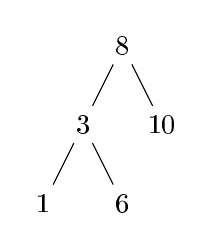
\begin{tikzpicture}[level distance=1cm,
    sibling distance=1cm]
  \node {8}
  child {
    node {3}
    child { node {1} }
    child { node {6} }
  }
  child { node {10} };
\end{tikzpicture}
\end{minipage}
\parbox[b][3.3cm][c]{3em}{\center$\Longrightarrow$}
\begin{minipage}[b][3.3cm][t]{.2\textwidth}
\begin{tikzpicture}[level distance=1cm,
    sibling distance=1cm]
  \node {8}
  child {
    node {3}
    child { node {1} }
    child {
      node {6}
      child { node {4} }
      child { edge from parent[draw=none] }
    }
  }
  child { node {10} };
\end{tikzpicture}
\end{minipage}
\parbox[b][3.3cm][c]{3em}{\center$\Longrightarrow$}
\begin{minipage}[b][3.3cm][t]{.3\textwidth}
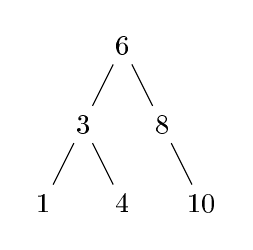
\begin{tikzpicture}[level distance=1cm,
    sibling distance=1cm]
  \node {6}
  child {
    node {3}
    child { node {1} }
    child { node {4} }
  }
  child {
    node {8}
    child { edge from parent[draw=none] }
    child { node {10} }
  };
\end{tikzpicture}
\end{minipage}
\end{center}
A 4-es beszúrása után a 6-os \pr{<} típusú lesz, a
3-as \pr{>} típusú, de probléma csak a legfelső
szinten jelentkezik, ahol a 8-as már eleve \pr{<}
típusú volt. Itt tehát az egész fára fog meghívódni
a forgató \pr{rebalance} operáció, aminek az
eredménye jobboldalt látszik.

\begin{program*}
% del_min_assoc(+Assoc0, ?Key, ?Val, -Assoc)
%                                         [semidet]
del_min_assoc(Tree, Key, Val, NewTree) :-
    del_min_assoc(Tree, Key, Val,
                  NewTree, _DepthChanged).

del_min_assoc(t(Key,Val,_B,t,R), Key, Val,
              R, yes) :- !.
del_min_assoc(t(K,V,B,L,R), Key, Val,
              NewTree, Changed) :-
    del_min_assoc(L, Key, Val, NewL, LeftChanged),
    deladjust(LeftChanged, t(K,V,B,NewL,R),
              left, NewTree, Changed).
\end{program*}
Kitörli a legkisebb kulcsú elemet. \pr{Val} a hozzá
tartozó érték, és az utolsó argumentum a törléssel
keletkezett AVL-fa. Ha a baloldali részfa üres,
akkor a keresett kulcs a gyökérben van, és az új fa
a jobboldali részfa lesz. Egyébként a baloldali
részfában végezzük rekurzívan a törlést, és utána
kiegyensúlyozzuk a \pr{deladjust} szabály
segítségével (ld.~lent).

\begin{program*}
% del_max_assoc(+Assoc0, ?Key, ?Val, -Assoc)
%                                         [semidet]
del_max_assoc(Tree, Key, Val, NewTree) :-
    del_max_assoc(Tree, Key, Val,
                  NewTree, _DepthChanged).

del_max_assoc(t(Key,Val,_B,L,t), Key, Val,
              L, yes) :- !.
del_max_assoc(t(K,V,B,L,R), Key, Val,
              NewTree, Changed) :-
    del_max_assoc(R, Key, Val, NewR, RightChanged),
    deladjust(RightChanged, t(K,V,B,L,NewR),
              right, NewTree, Changed).
\end{program*}
Ugyanez, csak a legnagyobb kulcsú elemmel és
jobboldali rekurzióval.

\begin{program*}
% del_assoc(+Key, +Assoc0, ?Value, -Assoc) [semidet]
del_assoc(Key, A0, Value, A) :-
    delete(A0, Key, Value, A, _).

delete(t(Key,Val,B,L,R), K, V,
       NewTree, WhatHasChanged) :-
    compare(Rel, K, Key),
    delete(Rel, t(Key,Val,B,L,R), K, V,
           NewTree, WhatHasChanged).

delete(=, t(Key,Val,_B,t,R), Key, Val, R, yes) :- !.
delete(=, t(Key,Val,_B,L,t), Key, Val, L, yes) :- !.
delete(=, t(Key,Val,>,L,R), Key, Val,
       NewTree, WhatHasChanged) :-
    del_min_assoc(R, K, V, NewR, RightHasChanged),
    deladjust(RightHasChanged, t(K,V,>,L,NewR),
              right, NewTree, WhatHasChanged),
    !.
delete(=, t(Key,Val,B,L,R), Key, Val,
       NewTree, WhatHasChanged) :-
    del_max_assoc(L, K, V, NewL, LeftHasChanged),
    deladjust(LeftHasChanged, t(K,V,B,NewL,R),
              left, NewTree, WhatHasChanged),
    !.

delete(<, t(Key,Val,B,L,R), K, V,
       NewTree, WhatHasChanged) :-
    delete(L, K, V, NewL, LeftHasChanged),
    deladjust(LeftHasChanged, t(Key,Val,B,NewL,R),
              left, NewTree, WhatHasChanged).
delete(>, t(Key,Val,B,L,R), K, V,
       NewTree, WhatHasChanged) :-
    delete(R, K, V, NewR, RightHasChanged),
    deladjust(RightHasChanged, t(Key,Val,B,L,NewR),
              right, NewTree, WhatHasChanged).
\end{program*}
Általános törlő operáció. Nézzük végig a
\pr{delete/6} egyes eseteit!
\begin{enumerate}
\item Keresett kulcs a gyökérben, baloldali részfa
  üres. Eredmény a jobboldali részfa.
\item Keresett kulcs a gyökérben, jobboldali részfa
  üres. Eredmény a baloldali részfa.
\item Keresett kulcs a gyökérben, és a jobboldali
  részfa mélyebb. Ekkor a jobboldali részfából
  kiveszi a legkisebb kulcsú elemet, és berakja a
  gyökérbe, majd kiegyensúlyozza a fát.
\item Keresett kulcs a gyökérben, és a jobboldali
  részfa nem mélyebb. Ekkor a baloldali részfából
  kiveszi a legnagyobb kulcsú elemet, és berakja a
  gyökérbe, majd kiegyensúlyozza a fát.
\item Keresett kulcs kisebb a gyökér
  kulcsánál. Rekurzív törlés a bal részfában, utána
  kiegyensúlyozás.
\item Keresett kulcs nagyobb a gyökér
  kulcsánál. Rekurzív törlés a jobb részfában, utána
  kiegyensúlyozás.
\end{enumerate}

\begin{program*}
deladjust(no, OldTree, _, OldTree, no).
deladjust(yes, t(Key,Val,B0,L,R), LoR,
          NewTree, RealChange) :-
    deltable(B0, LoR, B1,
             WhatHasChanged, ToBeRebalanced),
    rebalance(ToBeRebalanced, t(Key,Val,B0,L,R), B1,
              NewTree, WhatHasChanged, RealChange).

deltable(-, right, <, no , no ) :- !.
deltable(-, left , >, no , no ) :- !.
deltable(<, right, -, yes, yes) :- !.
deltable(<, left , -, yes, no ) :- !.
deltable(>, right, -, yes, no ) :- !.
deltable(>, left , -, yes, yes) :- !.
\end{program*}
Teljesen hasonló a beszúrás utáni \pr{adjust}
szabályhoz, csak törlés után.

\begin{program*}
rebalance(no, t(K,V,_,L,R), B, t(K,V,B,L,R),
          Changed, Changed).
rebalance(yes, OldTree, _, NewTree,
          _, RealChange) :-
    avl_geq(OldTree, NewTree, RealChange).
\end{program*}
Elérkeztünk az AVL-fák lelkéhez, a forgató
\pr{rebalance} szabályhoz. Az első argumentum azt
mondja meg, hogy szükség van-e forgatásra. Ha ez
\pr{no}, akkor a fa lényegileg nem változik, csak az
egyensúly-szimbólumot állítja be a harmadik
argumentumban kapott értékre (ami a megfelelő
táblázatból lett kiolvasva). Az utolsó argumentum
azt mutatja, hogy a fa mélysége megváltozott-e, és
ha nem történik forgatás, akkor csak átmásolja a
beszúrás/törlés során megállapított értéket.

A tényleges forgatást az \pr{avl\_geq} végzi, aminek
mindössze 3 argumentuma van: a régi fa, a forgatás
után keletkező új fa, és hogy a forgatás során
változott-e a fa mélysége.

\begin{program*}
avl_geq(t(A,VA,>,Alpha,t(B,VB,>,Beta,Gamma)),
        t(B,VB,-,t(A,VA,-,Alpha,Beta),Gamma),
        yes) :- !.
avl_geq(t(A,VA,>,Alpha,t(B,VB,-,Beta,Gamma)),
        t(B,VB,<,t(A,VA,>,Alpha,Beta),Gamma),
        no) :- !.
avl_geq(t(B,VB,<,t(A,VA,<,Alpha,Beta),Gamma),
        t(A,VA,-,Alpha,t(B,VB,-,Beta,Gamma)),
        yes) :- !.
avl_geq(t(B,VB,<,t(A,VA,-,Alpha,Beta),Gamma),
        t(A,VA,>,Alpha,t(B,VB,<,Beta,Gamma)),
        no) :- !.
avl_geq(t(A,VA,>,Alpha,
            t(B,VB,<,t(X,VX,B1,Beta,Gamma),Delta)),
        t(X,VX,-,t(A,VA,B2,Alpha,Beta),
            t(B,VB,B3,Gamma,Delta)),
        yes) :-
    !,
    table2(B1, B2, B3).
avl_geq(t(B,VB,<,
            t(A,VA,>,Alpha,t(X,VX,B1,Beta,Gamma)),
            Delta),
        t(X,VX,-,t(A,VA,B2,Alpha,Beta),
            t(B,VB,B3,Gamma,Delta)),
        yes) :-
    !,
    table2(B1, B2, B3).

table2(< ,- ,> ).
table2(> ,< ,- ).
table2(- ,- ,- ).
\end{program*}
Nézzük végig az egyes eseteket!
\begin{enumerate}
\item \pr{>/>}: a jobboldali részfa túl mély, és
  annak a jobboldali részfája a mélyebb. A forgatás
  hatására a mélység csökken.
\begin{center}
\begin{minipage}[b][2.5cm][t]{.3\textwidth}
\begin{tikzpicture}[level distance=1cm]
  \node {A}
  child { node {$\alpha$} }
  child {
    node {B}
    child { node {$\beta$} }
    child { node {$\gamma$} }
  };
\end{tikzpicture}
\end{minipage}
\parbox[b][3cm][c]{2.5em}{\center$\Longrightarrow$}
\begin{minipage}[b][2.5cm][t]{.3\textwidth}
\begin{tikzpicture}[level distance=1cm]
  \node {B}
  child {
    node {A}
    child { node {$\alpha$} }
    child { node {$\beta$} }
  }
  child { node {$\gamma$} };
\end{tikzpicture}
\end{minipage}
\end{center}
\item \pr{>/-}: a jobboldali részfa túl mély, és az
  egyensúlyban van. Ez csak baloldali törlés után
  jöhet létre. A forgatás megegyezik az előzővel, de
  ilyenkor a mélység nem változik.
\item \pr{</<}: az 1-es tükrözve.
\item \pr{</-}: a 2-es tükrözve.
\item \pr{>/<}: a jobboldali részfa túl mély, és
  annak a baloldali részfája a mélyebb. A forgatás
  hatására a mélység csökken. Az \pr{A}-nál és
  \pr{B}-nél levő egyensúly-szimbólumokat az
  \pr{X}-nél levő alapján a \pr{table2} táblázat
  adja meg.
\begin{center}
\begin{minipage}[b][3.5cm][t]{.25\textwidth}
\begin{tikzpicture}[level distance=1cm]
  \node {A}
  child { node {$\alpha$} }
  child {
    node {B}
    child {
      node {X}
      child { node {$\beta$} }
      child { node {$\gamma$} }
    }
    child { node {$\delta$} }
  };
\end{tikzpicture}
\end{minipage}
\parbox[b][3cm][c]{3.5em}{\center$\Longrightarrow$}
\begin{minipage}[b][3.5cm][t]{.45\textwidth}
\begin{tikzpicture}[level distance=1cm,
    level 1/.style={sibling distance=2.5cm},
    level 2/.style={sibling distance=1.5cm}]
  \node {X}
  child {
    node {A}
    child { node {$\alpha$} }
    child { node {$\beta$} }
  }
  child {
    node {B}
    child { node {$\gamma$} }
    child { node {$\delta$} }
  };
\end{tikzpicture}
\end{minipage}
\end{center}
\item \pr{</>}: az 5-ös tükrözve (ilyen volt a fenti
  beszúrásos példa).
\end{enumerate}

Itt érdemes megjegyezni, hogy a mélységcsökkenést
jelző utolsó argumentumot csak a \pr{deladjust}
veszi figyelembe, az \pr{adjust} nem. Ennek az az
oka, hogy ha beszúráskor nőne a mélység, akkor a
forgatás azt mindig kompenzálja, tehát végül az
eredeti állapothoz képest a mélység nem
változik. Ezzel szemben törlésnél ha forgatásra van
szükség, akkor csak ettől függ, hogy a mélység
csökken-e.

Ezzel vége a könyvtár forráskódjának. Ez egy szép,
jól érthető program, ami kevés külső definíciót
használ, ugyanakkor rendkívül tanulságos.

\section{Projekt: prioritásos sor}
Egy másik gyakran szükséges adatszerkezet a
\emph{prioritásos sor}, amiben minden elemhez egy
prioritást rendelünk, és mindig a legmagasabb
prioritásút vesszük ki belőle. A következő
szabályokkal kezelhető:
\begin{itemize}
\item \pr{üres\_sor(?Sor)} [semidet]
\item \pr{sorba\_tesz(+Sor, +Prioritás, ?Elem, -Sor1)} [det]
\item \pr{maximum\_elem(+Sor, ?Elem)} [semidet]
\item \pr{maximumot\_kivesz(+Sor, -Prioritás, ?Elem, -Sor1)} [semidet]
\end{itemize}
A kényelmes használat kedvéért még érdemes
listából/listává átváltó szabáyokat is készíteni
(ahol a lista \pr{Prioritás-Elem} párokból áll):
\begin{itemize}
\item \pr{listából\_sor(+Lista, -Sor)} [det]
\item \pr{sorból\_lista(+Sor, -Lista)} [det]
\end{itemize}
Ennek egy egyszerű megoldása az, hogy a betevés
sorrendjében egy listában tároljuk az elemeket --
ebben az esetben a maximum megkeresése ill. a sorból
kivétel $O(n)$ műveletigényű lesz. Egy másik
lehetőség, hogy az elemeket mindig csökkenő
sorrendben tároljuk; ekkor az új elem betevése lesz
$O(n)$-es komplexitású.

Egy hatékonyabb módszert kapunk, ha itt is egy fát
használunk. Ebben a fában a csúcsokból nem csak
kettő, hanem több ág is indulhat, és csak azt várjuk
el, hogy a csúcsban levő prioritás legalább akkora
legyen, mint az alatta levő részfák maximum
prioritása, így a maximum mindig a gyökérben
lesz. Ezt ,,párosító kupacnak'' nevezik.
\index{kupac!párosító}

Két ilyen fa egybeolvasztása nagyon egyszerű:
megnézzük, hogy melyik gyökerének nagyobb a
prioritása, és az marad a gyökér, a másik pedig ez
alá kerül új részfaként. A beszúrás is ennek egy
speciális esete, ahol a beszúrt elem egy olyan fa,
aminek csak gyökere van.

Az egyetlen bonyolultabb -- $O(\log n)$ komplexitású
-- művelet a maximális prioritású elem
kivétele. Ilyenkor az összes alatta levő részfát
egybe kell olvasztani, amíg csak egy nem marad. Ez
sokféleképp megtehető, és a különböző módszerek más
jellegű fákat eredményeznek. A klasszikus megoldás
az, hogy a részfákat először balról jobbra páronként
egybeolvasztjuk (innen a nevében a \emph{párosító}),
és utána a jobboldalitól elindulva a már
egybeolvasztott párokat egyenként
hozzáolvasztjuk. (Ez rekurzív módon nagyon
egyszerűen megfogalmazható.)

Nézzünk egy példát! Jelölje \pr{P-[P1,P2,..,Pn]} azt
a fát, aminek a gyökerében \pr{P}, az alatta levő
részfák gyökerében pedig \pr{Pi} prioritások vannak
(a további, érdektelen részfákat \pr{..} jelöli):
\begin{query}
10-[5,8,2,8,10,1,3]
\end{query}
Maximumkivétel $\Rightarrow$ 7 különálló fa:
\begin{query}
5-[..] 8-[..] 2-[..] 8-[..] 10-[..] 1-[..] 3-[..]
\end{query}
Párosítás balról jobbra $\Rightarrow$ 4 különálló
fa:
\begin{query}
8-[5,..] 8-[2,..] 10-[1,..] 3-[..]
\end{query}
Egyesítés jobbról balra, amíg csak 1 marad:
\begin{query}
8-[5,..] 8-[2,..] 10-[3,1,..]

8-[5,..] 10-[8-[2,..],3,1,..]

10-[8-[5,..],8-[2,..],3,1,..]
\end{query}
\begin{problem}
Készíts egy prioritásos sor adatszerkezetet párosító
kupaccal!
\end{problem}


\backmatter

Blabla


% -*- fill-column: 52 -*-
% (local-set-key (kbd "C-c C-f") 'display-fill-column-indicator-mode)

\chapter{A feladatok megoldásai}
\subsubsection*{1.~feladat}
\begin{query}
?- szülő(huszajn, X).
false

?- szülő(X, huszajn).
X = ali ;
X = fátima

?- szülő(ámna, X), szülő(X, fátima).
X = mohamed

?- szülő(ámna, X), szülő(X, Y), szülő(Y, haszan).
X = mohamed,
Y = fátima
\end{query}
\subsubsection*{2.~feladat}
\begin{query}
?- szülő(X, ali).
?- szülő(umáma, X).
?- szülő(X, zajnab), szülő(Nagyszülő, X).
\end{query}
\subsubsection*{4.~feladat}
\begin{program}
boldog(X) :- vangyereke(X).
kétgyerekes(X) :- szülő(X, Y), fivér(Y, _).
\end{program}
\subsubsection*{5.~feladat}
\begin{program}
unoka(X, Y) :- nagyszülő(Y, X).
\end{program}
\subsubsection*{6.~feladat}
\begin{program}
nővér(X, Y) :-
    nő(X),
    szülő(Z, X), szülő(Z, Y),
    X \= Y.
nagynéni(X, Y) :- nővér(X, Z), szülő(Z, Y).
\end{program}
\begin{query}
?- nagynéni(zajnab, X), férfi(X).
\end{query}
\subsubsection*{7.~feladat}
Jó a definíció; X őse Z-nek, ha (i) X szülője Z-nek, vagy (ii) X őse Z szülőjének.
\subsubsection*{8.~feladat}
Változó; atom; atom; változó; atom; struktúra; szám; (hibás); struktúra; (hibás).
\subsubsection*{9.~feladat}
Erre a feladatra nincs \emph{egyetlenegy} jó megoldás; különböző alkalmazásokhoz
más és más leírási módok lehetnek kényelmesebbek.
\begin{itemize}
\item Egy tengelyekkel párhuzamos téglalapot le lehet (pl.) írni a bal
  felső és jobb alsó sarkával, tehát \pr{téglalap(BalFelső, JobbAlsó)},
  ahol \pr{BalFelső} és \pr{JobbAlsó} pontok: \pr{pont(X, Y)}.  Ha a
  téglalap a tengelyekkel nem párhuzamos, akkor a legegyszerűbb talán
  mind a négy csúcspontot felsorolni (bár ez redundáns).
  Egy másik lehetőség, hogy egy irányított szakasszal és egy hosszal
  írjuk le: \pr{téglalap( szakasz(P1,P2),Hossz)}; ez alapján a téglalap
  úgy szerkeszthető meg, hogy a szakasz
  lerajzolása után derékszögben balra fordulunk,
  és onnan felmérjük a hosszt, a negyedik csúcs pedig már adódik.
\item Egy négyzetet mindig le lehet írni a bal felső és jobb alsó
  sarokkal, de lehet pl.~a középponttal és egy csúcsponttal is;
  tengelyekkel párhuzamos esetben elég a középpont és a csúcsok ettől
  való távolsága is.
\item Egy kört is reprezentálhat a befoglaló négyzete, de megadható a
  középpontja és a sugara által is: \pr{kör(Középpont, Sugár)},
  pl.~\pr{kör(pont(1,2),3)}.
\end{itemize}
\subsubsection*{10.~feladat}
\begin{program}
vízszintes(szakasz(pont(_,Y),pont(_,Y))).
\end{program}
\begin{query}
?- vízszintes(S), függőleges(S).
S = szakasz(pont(_X,_Y),pont(_X,_Y)).
\end{query}
Tehát a ponttá degenerált szakasz ilyen.
\subsubsection*{11.~feladat}
Igen (\pr{A=1,B=2}); nem; nem; igen (\pr{D=2,E=2});
nem;
igen (\pr{P1= pont(-1,0),P2=pont(1,0),P3=pont(0,Y)}).
\subsubsection*{12.~feladat}
A megoldás függ a választott reprezentációtól.
Ha a négy csúcsponttal
írtuk le:
\begin{program}
tengelytéglalap(téglalap(A,B,_,_)) :-
    függőleges(szakasz(P1,P2)).
tengelytéglalap(téglalap(_,B,C,_)) :-
    függőleges(szakasz(P2,P3)).
\end{program}
Ha az irányított szakasz és hossz megoldást
választottuk:
\begin{program}
tengelytéglalap(téglalap(S,_)) :- függőleges(S).
tengelytéglalap(téglalap(S,_)) :- vízszintes(S).
\end{program}
Természetesen sok más megoldás is elképzelhető.
\subsubsection*{13.~feladat}
\begin{program}
kiolvas(1, egy).
kiolvas(2, kettő).
kiolvas(3, három).
\end{program}
\subsubsection*{14.~feladat}
\begin{query}
?- f(s(1), A).
A = kettő.
\end{query}
Csak a második szabállyal egyesíthető.

\begin{query}
?- f(s(s(1)), kettő).
false.
\end{query}
Nincsen egyesíthető szabály.

\begin{query}
?- f(s(s(s(s(s(s(1)))))), C).
C = egy.
\end{query}
Nézzük ezt meg lépésenként.
Az eredeti kérdés csak a negyedik szabállyal egyesíthető;
egyesítés után az
\begin{query}
?- f(s(s(s(1))), C).
\end{query}
kérdést kell megválaszolni, ami ismét a negyedik szabállyal
egyesíthető, tehát:
\begin{query}
?- f(1, C).
\end{query}
Ez pedig az első szabály alapján adja az eredményt.

\begin{query}
?- f(D, három).
D = s(s(1)) ;
D = s(s(s(s(s(1))))) ;
D = s(s(s(s(s(s(s(s(1)))))))) ;
...
\end{query}
A harmadik szabály adja az első megoldást.
A negyedik szabály szerint, ha
\begin{query}
?- f(X, három).
\end{query}
teljesül, akkor \pr{D = s(s(s(X)))}, ez alapján
minden olyan \pr{D} megoldás lesz, ahol $3n+2$ db.~\pr{s}
szerepel.
\subsubsection*{15.~feladat}
\begin{query}
trace, nagy(X), sötét(X), notrace.
Call: nagy(_5078)
Exit: nagy(medve)
Call: sötét(medve)
  Call: fekete(medve)
  Fail: fekete(medve)
Redo: sötét(medve)
  Call: barna(medve)
  Exit: barna(medve)
Exit: sötét(medve)
X = medve 
\end{query}
\subsubsection*{16.~feladat}
A nyomkövetés a \pr{fekete(X)} kielégítésétől indul.
A \pr{notrace} hozzáadásával a nyomkövetés csak addig tart,
amíg el nem jut a \pr{sötét} második szabályához:
\begin{query}
?- sötét(X), nagy(X).
  Call: fekete(_4284)
  Exit: fekete(macska)
Exit: sötét(macska)
Call: nagy(macska)
Fail: nagy(macska)
Redo: sötét(_4284)
X = medve.
\end{query}
\subsubsection*{17.~feladat}
Amikor további bizonyítást keresünk, a második szabály alapján
Fátimának egy másik ősét (nem Mohamedet) fogja keresni,
akiről aztán majd be akarja látni, hogy Abdulla gyermeke.

Ekkor azonban eljutunk a második szabályhoz úgy, hogy az \pr{X}
ismeretlen, és a szabály szerint az
\begin{query}
?- ős3(X, fátima).
\end{query}
kérdés megválaszolásához először meg kell válaszolni az
\begin{query}
?- ős3(Y, fátima).
\end{query}
kérdést -- ez viszont nyilvánvalóan egy végtelen rekurzió.
\subsubsection*{18.~feladat}
\begin{program}
kivesz3(X, Y) :- hozzáfűz(Y, [_,_,_], X).
\end{program}
\subsubsection*{19.~feladat}
\begin{program}
kivesz33(X, Y) :- kivesz3(X, [_,_,_|Y]).
\end{program}
\subsubsection*{20.~feladat}
Hozzáfűzéssel:
\begin{program}
utolsó(X,Y) :- hozzáfűz(_,[Y],X).
\end{program}
Anélkül:
\begin{program}
utolsó(X, [X]). 
utolsó(X, [_|M]) :- utolsó(X, M). 
\end{program}
\subsubsection*{21.~feladat}
\begin{program}
páros_hosszú([]). 
páros_hosszú([_|M]) :- páratlan_hosszú(M). 
páratlan_hosszú([_|M]) :- páros_hosszú(M). 
\end{program}
\subsubsection*{22.~feladat}
\begin{program}
fordított([], []). 
fordított([X|M], F) :-
    fordított(M, L), hozzáfűz(L, [X], F).
\end{program}
\subsubsection*{23.~feladat}
\begin{program}
palindróma(X) :- fordított(X, X).
\end{program}
\subsubsection*{24.~feladat}
\begin{program}
forgat([X|M], Y) :- hozzáfűz(M, [X], Y). 
\end{program}
\subsubsection*{25.~feladat}
\begin{program}
részhalmaz([], []).
részhalmaz([X|M], [X|R]) :- részhalmaz(M, R).
részhalmaz([_|M], R) :- részhalmaz(M, R).
\end{program}
\subsubsection*{26.~feladat}
\begin{program}
ugyanolyan_hosszú([], []). 
ugyanolyan_hosszú([_|M], [_|N]) :-
    ugyanolyan_hosszú(M, N). 
\end{program}
\subsubsection*{27.~feladat}
\begin{program}
lapít([], []). 
lapít([X|M], Y) :-
    lapít(X, X1), lapít(M, M1),
    hozzáfűz(X1, M1, Y). 
lapít(X, [X]) :- X \= [], X \= [_|_]. 
\end{program}
\subsubsection*{28.~feladat}
\begin{query}
?- t(0+1, A).
A = 1+0.
?- t(0+1+1, B).
B = 1+1+0
?- t(1+0+1+1+1, C).
C = 1+1+1+1+0
?- t(D, 1+1+1+0).
D = 1+1+0+1 ;
D = 1+0+1+1 ;
D = 0+1+1+1
\end{query}
\subsubsection*{29.~feladat}
\begin{program}
max(A, B, A) :- A >= B. 
max(A, B, B) :- A < B. 
\end{program}
\subsubsection*{30.~feladat}
\begin{program}
maximum([X], X).
maximum([X,Y|M], Z) :-
    maximum([Y|M], X1), max(X, X1, Z).
\end{program}
\subsubsection*{31.~feladat}
\begin{program}
összeg([], 0). 
összeg([X|M], N):- összeg(M, N1), N is N1 + X. 
\end{program}
\subsubsection*{32.~feladat}
\begin{program}
növekvő([_]). 
növekvő([A,B|M]) :- A < B, növekvő([B|M]). 
\end{program}
\subsubsection*{33.~feladat}
\begin{program}
részösszeg(L, N, X) :-
    részhalmaz(L, X), összeg(X, N).
\end{program}
\subsubsection*{34.~feladat}
\begin{program}
között(A, B, A) :- A =< B. 
között(A, B, X) :-
    A < B, A1 is A + 1,
    között(A1, B, X). 
\end{program}
\subsubsection*{35.~feladat}
\begin{program}
:- op(600, xfx, :=). 
:- op(700, xfx, egyébként). 
:- op(800, xfx, akkor). 
:- op(900, fx, ha). 
ha X > Y akkor Z := V egyébként _ :- X > Y, Z = V. 
ha X > Y akkor _ egyébként Z := V :- X =< Y, Z = V. 
\end{program}
\subsubsection*{36.~feladat}
\begin{query}
?- p(X).
X = 1 ;
X = 2
?- p(X), p(Y).
X = 1, Y = 1 ;
X = 1, Y = 2 ;
X = 2, Y = 1 ;
X = 2, Y = 2
?- p(X), !, p(Y).
X = 1, Y = 1 ;
X = 1, Y = 2
\end{query}
\subsubsection*{37.~feladat}
\begin{program}
szétoszt(_, [], [], []) :- !. 
szétoszt(X, [Y|M], K, [Y|N]) :-
    X =< Y, !, szétoszt(X, M, K, N). 
szétoszt(X, [Y|M], [Y|K], N) :-
    X > Y, !, szétoszt(X, M, K, N). 
\end{program}
\subsubsection*{38.~feladat}
\begin{query}
?- tartalmaz(X, Jelöltek),
   \+ tartalmaz(X, Kiesettek).
\end{query}
\subsubsection*{39.~feladat}
\begin{program}
különbség([], _, []). 
különbség([X|M], Y, Z) :-
    tartalmaz(X, Y), !, különbség(M, Y, Z). 
különbség([X|M], Y, [X|Z]) :- különbség(M, Y, Z).
\end{program}
\subsubsection*{40.~feladat}
\begin{program}
egyesíthető([], _, []) :- !. 
egyesíthető([X|M], Y, L) :-
    \+(X = Y), !, egyesíthető(M, Y, L). 
egyesíthető([X|M], Y, [X|L]) :-
    egyesíthető(M, Y, L). 
\end{program}
Ha tagadás nélkül ellenőriznénk az egyesíthetőséget,
akkor el is végezné az egyesítést:
\begin{program}
egyesíthető_rossz([], _, []) :- !. 
egyesíthető_rossz([X|M], Y, [X|L]) :-
    X = Y, !, egyesíthető_rossz(M, Y, L). 
egyesíthető_rossz([X|M], Y, L) :-
    egyesíthető_rossz(M, Y, L). 
\end{program}
\begin{query}
?- egyesíthető_rossz([X,b,t(Y)], t(a), L).
X = t(a),
Y = a,
L = [t(a), t(a)].
\end{query}
\subsubsection*{41.~feladat}
\begin{program}
katamino(M, Ak) :-
    hossz(Ak, H), N is H * 5 // M,
    H * 5 =:= N * M,
    kirak(N-M, Ak, X), kiír(N-M, X).

kirak(N-M, Ak, X) :- kirak(Ak, N-M, [], X).

kirak([], _, T, T).
kirak(Ak, N-M, T, X) :-
    első_lyuk(N-M, T, P),
    töröl(A, Ak, Ak1),
    letesz(A, P, N-M, T, T1),
    kirak(Ak1, N-M, T1, X).

első_lyuk(N-M, T, X-Y) :-
    között(1, N, X), között(1, M, Y),
    \+ tartalmaz(h(X-Y,_), T), !.

letesz(A, X-Y, N-M, T, T1) :-
    alakzat(A, [_-Dy|Dk]),
    Y1 is Y - Dy, Y1 > 0,
    letesz(A, X-Y1, Dk, N-M, [h(X-Y,A)|T], T1).

letesz(_, _, [], _, T, T).
letesz(A, X-Y, [Dx-Dy|Dk], N-M, T, T1) :-
    X1 is X + Dx, között(1, N, X1),
    Y1 is Y + Dy, között(1, M, Y1),
    \+ tartalmaz(h(X1-Y1,_), T),
    letesz(A, X-Y, Dk, N-M, [h(X1-Y1,A)|T], T1).

kiír(N-M, T) :- kiír(N-M, 1-M, T).

kiír(_, _-0, _).
kiír(N-M, X-Y, T) :-
    Y =< M, X > N, Y1 is Y - 1, nl,
    kiír(N-M, 1-Y1, T).
kiír(N-M, X-Y, T) :-
    Y =< M, X =< N,
    tartalmaz(h(X-Y,A), T),
    write(A), write(' '),
    X1 is X + 1,
    kiír(N-M, X1-Y, T).
\end{program}
(A program további része változatlan.)
\begin{query}
?- katamino(3, [k,p,c,w,l,y,i,r,v,z,+,t]).
c c + i i i i i k k k r t w y y y y z v 
c + + + p p l k k r r r t w w y z z z v 
c c + p p p l l l l r t t t w w z v v v 
true 

?- katamino(4, [k,p,c,w,l,y,i,r,v,z,+,t]).
p p z v v v c c c w w t t t y 
p p z z z v c r c + w w t y y 
p k k k z v r r + + + w t l y 
k k i i i i i r r + l l l l y 
true 

?- katamino(5, [k,p,c,w,l,y,i,r,v,z,+,t]).
c c c r l l l l y y y y 
c k c r r w t l + y z z 
k k r r w w t + + + z v 
k p p w w t t t + z z v 
k p p p i i i i i v v v 
true 

?- katamino(6, [k,p,c,w,l,y,i,r,v,z,+,t]).
p p y y y y z v v v 
p p l l y + z z z v 
p k l w + + + r z v 
k k l w w + r r r t 
k c l c w w r t t t 
k c c c i i i i i t 
true 
\end{query}
\subsubsection*{42.~feladat}
\begin{program}
lapít(X, Y) :- lapít_kl(X, Y-[]).

lapít_kl([], Y-Y).
lapít_kl([X|M], Y-A) :-
    lapít_kl(M, A1-A), lapít_kl(X, Y-A1).
lapít_kl(X, [X|A]-A) :- X \= [], X \= [_|_].
\end{program}
\subsubsection*{43.~feladat}
\begin{program}
holland(X, PFK) :- holland_kl(X, PFK-FK, FK-K, K-[]).

holland_kl([], P-P, F-F, K-K). 
holland_kl([piros(X)|M], [piros(X)|P]-P1, F, K) :-
    holland_kl(M, P-P1, F, K). 
holland_kl([fehér(X)|M], P, [fehér(X)|F]-F1, K) :-
    holland_kl(M, P, F-F1, K). 
holland_kl([kék(X)|M], P, F, [kék(X)|K]-K1) :-
    holland_kl(M, P, F, K-K1). 
\end{program}
\subsubsection*{44.~feladat}
A programban a \pr{k}-végű változónevek listákat
jelölnek, például \pr{Xk} (,,\pr{X}-ek'').%
\footnote{Angolul erre az \pr{s} végződést
használják.}
\begin{program}
egyszerűsít(Kifejezés, Megoldás) :-
    változók(Kifejezés, Változók, Konstansok),
    számol(Változók, Számolt),
    összeg(Konstansok, N),
    felépít(Számolt, N, Megoldás).

összeg([], 0).
összeg([X|Xk], N):- összeg(Xk, N1), N is N1 + X.

felépít([], N, N) :- !.
felépít(Számolt, N, Megoldás) :-
    felépít(Számolt, Érték),
    ( N =:= 0, !, Megoldás = Érték
    ; N =\= 0, Megoldás = Érték + N
    ).

% Felépíti a kifejezés szimbolikus részét
felépít([v(X,1)], X) :- !.
felépít([v(X,K)], K*X) :- K > 1, !.
felépít([V1,V2|Vk], E2+E1) :-
    felépít([V1], E1),
    felépít([V2|Vk], E2).

% változók(+Kifejezés, -Változók, -Konstansok)
%   Szétválogatja a változókat és konstansokat.
változók(X, [X], []) :- atom(X), !.
változók(X, [], [X]) :- number(X), !.
változók(Xk+X, [X|Vk], Kk) :-
    atom(X), !, változók(Xk, Vk, Kk).
változók(Xk+X, Vk, [X|Kk]) :-
    number(X), változók(Xk, Vk, Kk).

% Megszámolja a változók előfordulásait,
% pl. [a,a,b,a,c,b] => [v(a,3),v(b,2),v(c,1)]
számol([], []).
számol([X|Xk], [v(X,N)|Zk]) :-
    számol_és_töröl(X, Xk, N, Yk),
    számol(Yk, Zk).

% számol_és_töröl(+X, +L, -N, -L1)
%   Megszámolja az X előfordulásait L-ben (N),
%   és kitörli őket, ennek eredménye az L1.
számol_és_töröl(_, [], 1, []) :- !.
számol_és_töröl(X, [X|Yk], N, Zk) :-
    !, számol_és_töröl(X, Yk, N1, Zk),
    N is N1 + 1.
számol_és_töröl(X, [Y|Yk], N, [Y|Zk]) :-
    X \= Y, számol_és_töröl(X, Yk, N, Zk).
\end{program}
\subsubsection*{45.~feladat}
\begin{program}
bagof(C, részhalmaz(X, C), L).
\end{program}


\printindex

\end{document}
